\documentclass[12pt]{book}

% \usepackage{algorithm}
% \usepackage{algpseudocode}
% \algrenewcommand\algorithmicrequire{\textbf{Input:}}
% \algrenewcommand\algorithmicensure{\textbf{Output:}}
% \algnewcommand\Not{\textbf{not} }
% \newcommand{\algorithmautorefname}{Algorithm} % autoref

\usepackage[inline]{enumitem}
\usepackage{adjustbox}
\usepackage[headings]{fullpage}
\usepackage{xargs}
\usepackage{xspace}
\usepackage[doublespacing]{setspace}

\usepackage{hyperref}
\def\chapterautorefname{Chapter}
\def\sectionautorefname{Section}
\def\subsectionautorefname{Section}
\def\subsubsectionautorefname{Section}

\usepackage{microtype}
\usepackage[T1]{fontenc}

\usepackage{wrapfig}
\usepackage[font={sf}]{caption}
\usepackage[subrefformat=parens]{subcaption}

\usepackage{multirow}

\usepackage{xcolor}
\usepackage{graphicx}
\graphicspath{{_build/}{figures/}}

\usepackage{amsmath}
\newtheorem{defn}{Definition}[chapter]
\newtheorem{thm}{Theorem}[chapter]
\newtheorem{proof}{Proof}[chapter]
\newtheorem{prop}{Proposition}[chapter]
\newtheorem{lmm}{Lemma}[chapter]
\newtheorem{ex}{Example}[chapter]

\setlength{\marginparwidth}{2cm}
\usepackage[textsize=tiny]{todonotes}
\newcommand\remy[2][]{\todo[color=orange, #1]{\sffamily #2}}

\usepackage{libertine}
\usepackage[libertine]{newtxmath}
\usepackage[scaled=.85]{DejaVuSansMono}

\usepackage{listings}
\lstset{
  columns=fullflexible,
  keepspaces=true,
  showstringspaces=false,
  stringstyle=\slshape\color{green!40!black},
  basicstyle=\ttfamily\small,
  language=Python,
  morekeywords={*, self},
  commentstyle=\slshape\color{black!60},
  tabsize=2,
}

\lstdefinelanguage{Rust}{
  sensitive,
  morecomment=[l]{//},
  morecomment=[s]{/*}{*/},
  moredelim=[s][{\itshape\color[rgb]{0,0,0.75}}]{\#[}{]},
  morestring=[b]{"},
  alsodigit={},
  alsoother={},
  alsoletter={!},
  % keywords
  otherkeywords={=>},
  morekeywords={break, continue, else, for, if, in, loop, match, return, while},
  morekeywords={as, const, let, move, mut, ref, static, unsafe},
  morekeywords={dyn, enum, fn, impl, Self, self, struct, trait, type, use, where},
  morekeywords={crate, extern, mod, pub, super},
  morekeywords={abstract, alignof, become, box, do, final, macro,
    offsetof, override, priv, proc, pure, sizeof, typeof, unsized, virtual, yield},
  % traits
  morekeywords=[2]{Send},
  % types
  morekeywords=[3]{bool, char, f32, f64, i8, i16, i32, i64, isize, str, u8, u16, u32, u64, unit, usize, i128, u128},
}%

\def\mytitle{Relational Programming}
\def\myauthor{Yisu Remy Wang}
\def\year{2023}

\title{\mytitle}
\author{\myauthor}

\newcommand\thesisstmt{%
  The future of programming is relational.%
}

\newcommand\Thesisstmt{\expandafter\MakeUppercase \thesisstmt}

% \newcommand{\missing}[1]{{\color{red}\bfseries [TODO]}}

% \newcommand{\etal}{et al.\xspace}

% \newcommand{\egg}{\texorpdfstring{\MakeLowercase{\texttt{egg}}}{\texttt{egg}}\xspace}
% \newcommand{\Egg}{\texorpdfstring{\MakeLowercase{\texttt{egg}}}{\texttt{egg}}\xspace}
% \newcommand{\egraphs}{\mbox{e-graphs}\xspace}
% \newcommand{\egraph}{\mbox{e-graph}\xspace}
% \newcommand{\Egraph}{\mbox{E-graph}\xspace}
% \newcommand{\Egraphs}{\mbox{E-graphs}\xspace}
% \newcommand{\eclass}{\mbox{e-class}\xspace}
% \newcommand{\Eclass}{\mbox{E-class}\xspace}
% \newcommand{\enode}{\mbox{e-node}\xspace}
% \newcommand{\eclasses}{\mbox{e-classes}\xspace}
% \newcommand{\enodes}{\mbox{e-nodes}\xspace}
% \newcommand{\Enodes}{\mbox{E-nodes}\xspace}
% % \newcommand{\regraph}{Regraph\xspace}
% % \newcommand{\Regraph}{Regraph\xspace}
% \newcommand{\sz}{Szalinski\xspace}
% \newcommand{\find}{\texttt{find}\xspace}

% \newcommand{\eqsat}{equality saturation\xspace}
% \newcommand{\Eqsat}{Equality saturation\xspace}

% \newcommand{\equivid}{\equiv_{\sf id}}
% \newcommand{\equivnode}{\equiv_{\sf node}}
% \newcommand{\equivterm}{\equiv_{\sf term}}

% \newcommand{\congrinv}{$\mathcal{I}_c$\xspace}

% \newcommand{\egglogo}[1][]{\protect\includegraphics[height=1em, #1]{egg.png} }
% \newcommand{\eggurl}{\url{https://github.com/mwillsey/egg}}

\newcommand\cse{Computer Science \& Engineering}
\newcommand\pgas{Paul G.\ Allen School of \cse}

% \newcommand{\CongrSpeedup}{\ensuremath{87.85\times}\xspace}
% \newcommand{\TotalSpeedup}{\ensuremath{20.96\times}\xspace}
% \newcommand{\RepairsR}{\ensuremath{0.98}\xspace}
% \newcommand{\RepairsP}{3.6e-47\xspace}
% \newcommand{\nEggTests}{32\xspace}
% \newcommand{\nEggTimeouts}{8\xspace}

%%% Local Variables:
%%% TeX-master: "thesis"
%%% End:

\usepackage{bm} % bold math fonts, e.g. $\bm \Sigma$ will give a bold-face $\Sigma$
% \usepackage{url}
% \usepackage{fullpage}

% \setlength{\marginparwidth}{2cm} % for todonotes
% \usepackage[colorinlistoftodos]{todonotes}

% % http://paultaylor.eu/diagrams/
% % https://www.jmilne.org/not/Mdiagrams.pdf
% \usepackage[small,nohug,heads=vee]{diagrams}
% \diagramstyle[labelstyle=\scriptstyle]

% \usepackage[ruled, noend]{algorithm2e}
\usepackage{enumitem}
% \usepackage{quiver}
% \usepackage{subcaption}

%%% package microtype recommended by Paul Beame who says:
%%%%% try including [it] in any of your latex documents.  You will find that
%%%%% not only is the result more compact without changing any spacing
%%%%% parameters, the number of overfull/underfull warnings drops, and it
%%%%% simply looks a lot better!
%%%%%
%%%%% Why it works:  Latex is not known for the beauty of its typography.  The
%%%%% biggest issue is that the amount of visible white space between words
%%%%% varies quite a lot line-to-line in a paragraph since inter-word spacing
%%%%% is the only thing that will stretch/shrink.   The microtype package also
%%%%% makes imperceptible changes to the inter-letter spacing within words
%%%%% and, with all those extra degrees of freedom, it can do a much better
%%%%% job of laying out paragraphs.
% \usepackage{microtype}

\newcommand{\yell}[1]{{\color{red} \textbf{#1}}}

\newcommand{\rai}{Relational\underline{AI}}

\newcommand{\gv}[1]{\ensuremath{\mbox{\boldmath$ #1 $}}}
\newcommand{\grad}[1]{\gv{\nabla} #1}
\newcommand{\norm}[1]{\|#1\|}
\newcommand{\set}[1]{\{#1\}}                    % Set (as in \set{1,2,3}).
\newcommand{\bag}[1]{\{\hspace{-1mm}\{#1\}\hspace{-1mm}\}}                    % bag (as in \bag{1,2,3}).
\newcommand{\setof}[2]{\{{#1}\mid{#2}\}}        % Set (as in \setof{x}{x>0}).
\newcommand{\bagof}[2]{\{\hspace{-1mm}\{{#1}\mid{#2}\}\hspace{-1mm}\}}        % Set (as in \setof{x}{x>0}).
\newcommand{\pr}{\mathop{\textnormal{Prob}}}    % Probability
\newcommand{\E}{\mathop{\mathbb E}}    % Probability
\newcommand{\dom}{\textsf{Dom}}
\newcommand{\id}{\textsf{ID}}
\newcommand{\codom}{\textsf{CoDom}}
\newcommand{\one}{\bm 1}
\newcommand{\degree}{\text{\sf deg}}
\newcommand{\critdegree}{\text{\sf critDeg}}
\newcommand{\monomial}{\text{\sf Mon}}
\newcommand{\cmonomial}{\text{\sf \#Mon}}
\newcommand{\sign}{\text{\sf sign}}
\newcommand{\lfp}{\text{\sf lfp}}
\newcommand{\lpfp}{\text{\sf lpfp}}
\newcommand{\pfp}{\text{\sf pfp}}

\newcommand{\inner}[1]{\langle #1 \rangle}
%%
\newcommand{\LB}{\textsf{LogicBlox}}
\newcommand{\faq}{\textsf{FAQ}}
\newcommand{\calB}{\mathcal B}
\newcommand{\calC}{\mathcal C}
\newcommand{\calH}{\mathcal H}
\newcommand{\calV}{[n]}
\newcommand{\calE}{\mathcal E}
\newcommand{\calD}{\mathcal D}
\newcommand{\calW}{\mathcal W}
\newcommand{\calF}{\mathcal F}
\newcommand{\calP}{\mathcal P}
\newcommand{\calM}{\mathcal M}
\newcommand{\calN}{\mathcal N}
\newcommand{\calL}{\mathcal L}
\newcommand{\calS}{\mathcal S}
\newcommand{\calT}{\mathcal T}

% \theoremstyle{plain}                   % default
% \newtheorem{thm}{Theorem}[section]
% \newtheorem{lmm}[thm]{Lemma}
% \newtheorem{prop}[thm]{Proposition}
% \newtheorem{cor}[thm]{Corollary}
% \newtheorem{defn}[thm]{Definition}

% \theoremstyle{definition}              % Examples and all
% \newtheorem{pbm}{Problem}
% \newtheorem{opm}{Question}
% \newtheorem{conj}[thm]{Conjecture}
% \newtheorem{ex}[thm]{Example}
% \newtheorem{exer}{Exercise}
% \newtheorem{alg}[thm]{Algorithm}
% \newtheorem{rmk}[thm]{Remark}
% \newtheorem{claim}{Claim}
% \newtheorem{note}{Note}

\newcommand{\defeq}{\stackrel{\text{def}}{=}}
\newcommand{\mineq}{\stackrel{\text{min}}{=}}
\newcommand{\maxeq}{\stackrel{\text{max}}{=}}
\newcommand{\dleq}{\mbox{ :- }}
\newcommand{\mult}{\cdot}

\newcommand{\B}{\mathbb B} % the Booleans
\newcommand{\Z}{\mathbb Z} % integers
\newcommand{\N}{\mathbb N} % the natural numbers
\newcommand{\Q}{\mathbb Q} % the rational numbers
\newcommand{\R}{\mathbb R} % the real numbers
\newcommand{\T}{\mathbb T} % \set{\bot,\top}
%\newcommand{\C}{\mathbb C} % complex numbers
\newcommand{\D}{\mathbf D} % bold-face D, used for generic domain
% \newcommand{\U}{\mathbf U} % the universe


\newcommand{\cd}{\text{ :- }}
\newcommand{\iter}{\texttt{iter}}
\newcommand{\datalogo}{\texorpdfstring{$\text{Datalog}^\circ$\xspace}{Datalogo}}
\newcommand{\trop}{\text{\sf Trop}}
% \newcommand{\tropset}{\text{\sf T}}

\newcommand{\ground}{\textsf{GA}}
\newcommand{\arity}{\textsf{arity}}
\newcommand{\adom}{\textsf{ADom}}
\newcommand{\inst}{\textsf{Inst}}

\newcommand{\floor}[1]{\lfloor#1\rfloor}
\newcommand{\ceil}[1]{\lceil#1\rceil}


\begin{document}
\pagestyle{empty}

% title and copyright pages
\begin{center}
  {\huge \mytitle}
  \vfill

  {\Large \myauthor}
  \vfill

  \begin{spacing}{1}
    A dissertation \\
    submitted in partial fulfillment of the \\
    requirements for the degree of
  \end{spacing}
  \vfill

  Doctor of Philosophy
  \vfill

  University of Washington \\
  \year
  \vfill

  Reading Commitee: \\
  Dan Suciu, Chair \\
  Zachary Tatlock \\
  Andrew Lumsdaine
  \vfill
  \begin{spacing}{1}
    Program Authorized to Offer Degree: \\
    \cse
  \end{spacing}
  \clearpage

  \textcopyright{} Copyright \year\\
  \myauthor
  \clearpage
\end{center}

\pagestyle{plain}
\setcounter{page}{1}
\pagenumbering{roman}

% abstract page
\begin{center}
  University of Washington \\[1em]
  \textbf{Abstract}        \\[1em]
  \mytitle                 \\[1em]
  \myauthor                \\[1em]

  % Supervisory Committee: \\[-0.5em]
  % Luis Ceze, Chair \qquad
  % Adriana Schulz   \qquad
  % Zachary Tatlock  \\[-0.5em]
  Chair of the Supervisory Committee: \\[-0.5em]
  Dan Suciu \\[-0.5em]
  \pgas
  \\[2em]
\end{center}
Relational programming.

%%% Local Variables:
%%% TeX-master: "./thesis"
%%% End:


\begin{spacing}{1.5}
  \tableofcontents
\end{spacing}

\chapter*{Acknowledgments}

Thank you!

\clearpage

\pagestyle{headings}
\setcounter{page}{1}
\pagenumbering{arabic}
\renewcommand{\chaptermark}[1]{\markboth{\sc{\chaptername\ \thechapter.\ #1}}{}}
\renewcommand{\sectionmark}[1]{\markright{\sc{\thesection.\ #1}}{}}
% \listoftodos
\chapter{Introduction}
\label{sec:intro}

Fifty years after its initial proposal by Edgar F. Codd,
 the relational model has cemeted its status as the de-facto data model 
 in nearly all modern databases.
It provides {\em data independence}, 
 which has allowed data systems to scale to unprecedented sizes
 while guaranteeing performance and correctness.
The success of the relational model is witnessed 
 by the popularity of SQL, 
 uniquitous in computing systems 
 from smartphones to data centers.

 Nevertheless, traditional relational databases are struggling 
  to meet the demands of modern data analytics.
Today's data analytics involve new kinds of data, 
 as well as new kinds of computation over such data. 
For example, machine learning workloads involve linear algebra operations
 running over data stored as matrices. 
For another example, graph analytics require iterative algorithms
 over graph data.
Running these workloads in existing relational databases 
 is both cumbersome and slow:
 SQL is a poor language for expressing the computation
 and the systems are not optimized for such workloads.

This dissertation is motivated by the question: 
{\em How can we renew relational database systems 
 to support modern data analytics?}
Towards that end, I propose a new language foundation
 for writing relational programs;
 a new algorithm for the relational join;
 and techniques to optimize relational queries. 
Together, these three ingredients make up 
 the basis for a new generation of relational systems
 that are more expressive and more efficient.
Using these systems,
 the analyst may author entire application programs
 instead of simple queries {\em relationally},
 entering the era of {\em relational programming}.

\section{Motivation and Contributions}
\label{sec:intro:motivation}

% For fifty years, the relational data model has been the main choice for
% representing, modeling, and processing data.  
The main query language for relational databases, SQL, 
 is found today in a wide range of applications and
 devices. 
%  from smart phones, to database servers, to distributed
%  cloud-based clusters.
The reason for its success is the {\em data
  independence principle}, which separates the declarative model from
the physical implementation~\cite{DBLP:journals/cacm/Codd70}, and
enables advanced implementation techniques, such as cost-based
optimizations, indices, materialized views, incremental view
maintenance, parallel evaluation, and many others, while keeping the
same simple, declarative interface to the data unchanged.

But analysts today often need to perform tasks that require
iteration over the data.
Gradient descent, clustering, page-rank, network centrality, inference
in knowledge graphs are some examples of common tasks in data science
that require iteration.  While SQL has introduced recursion since 1999
(through Common Table Expressions, CTE), it has many cumbersome
limitations and is little used in practice~\cite{frankmcsherry-2022}.

The need to support recursion in a declarative language led to the
development of Datalog in the mid 80s~\cite{DBLP:conf/pods/Vianu21}.
Datalog adds recursion to the relational query language, yet enjoys several elegant
properties: it has a simple, declarative semantics; its na\"ive
bottom-up evaluation algorithm always terminates; and it admits a few
powerful optimizations, such as semi-na\"ive evaluation and magic set
rewriting.  Datalog has been extensively studied in the literature;
see~\cite{DBLP:journals/ftdb/GreenHLZ13} for a survey
and~\cite{DBLP:books/mc/18/MaierTKW18,DBLP:conf/pods/Vianu21} for historical notes.
We will also briefly review the semantics and execution of Datalog in
 Chapter~\ref{chap:background}.

However, Datalog is not the answer to modern needs, because it only
supports monotone queries over sets.  Most tasks in data science today
require the interleaving of recursion and aggregate computation.
Aggregates are not monotone under set inclusion, and therefore they
are not supported by the framework of pure Datalog.  Neither SQL'99
nor popular open-source Datalog systems like
Souffl\'e~\cite{DBLP:conf/cav/JordanSS16} allow recursive queries to
have aggregates.  While several proposals have been made to extend
Datalog with
aggregation~\cite{DBLP:conf/pods/GangulyGZ91,DBLP:conf/pods/RossS92,DBLP:journals/jcss/GangulyGZ95,DBLP:journals/vldb/MazuranSZ13,DBLP:conf/icde/ShkapskyYZ15,DBLP:conf/sigmod/ShkapskyYICCZ16,DBLP:conf/amw/ZanioloYDI16,DBLP:journals/tplp/ZanioloYDSCI17,DBLP:conf/amw/ZanioloYIDSC18,DBLP:journals/tplp/CondieDISYZ18,DBLP:conf/sigmod/0001WMSYDZ19,DBLP:journals/corr/abs-1910-08888,DBLP:journals/corr/abs-1909-08249,DBLP:journals/debu/ZanioloD0LL021},
these extensions are at odds with the elegant properties of Datalog
and have not been adopted by either Datalog systems or SQL engines.

\textbf{
The first contribution of this dissertation is a foundation for a query language that
supports both recursion and aggregation.}  
Our language, called \datalogo, 
 retains many of the elegant properties of Datalog,
 while extending its expressiveness to support aggregation.
Our proposal is based on the
concept of $K$-relations, introduced in a seminal
paper by Green, Karvounarakis, and Tannen~\cite{DBLP:conf/pods/GreenKT07}.
In a $K$-relation, tuples are
mapped to a fixed semiring. Standard relations (sets) are
$\B$-relations where tuples are mapped to the Boolean semiring $\B$,
relations with duplicates (bags) are $\N$-relations, sparse tensors
are $\R$-relations, and so on.  Queries over $K$-relations are the
familiar relational queries, where the operations $\wedge, \vee$ are
replaced by the operations $\otimes, \oplus$ in the semiring;
importantly, an existential quantifier $\exists$ becomes an
$\oplus$-aggregate operator.
$K$-relations are a very powerful abstraction, because they open up
the possibility of adapting query processing and optimization
techniques to other domains~\cite{DBLP:conf/pods/KhamisNR16}.

To evaluate any relational program, 
 including \datalogo programs,
 classic Datalog programs, 
 or even SQL queries without recursion, 
 the key operation is the relational join.
The join allows us to combine data from different sources, 
 as well as compose computation from multiple programs.
Most mainstream databases today evaluate a query 
 by joining two relations at a time.
In other words, they implement {\em binary join} algorithms.
Over the last decade, worst-case optimal join (\WCOJ)~\cite{
  DBLP:conf/pods/NgoPRR12,
  DBLP:conf/icdt/Veldhuizen14, 
  DBLP:journals/sigmod/NgoRR13, 
  DBLP:conf/pods/000118}
 has emerged as
 a breakthrough in the design of efficient join algorithms.  
It can be
asymptotically faster than traditional binary joins, all the while
remaining simple to understand and
implement~\cite{DBLP:journals/sigmod/NgoRR13}.  
\WCOJ has opened up a flourishing field of research, leading to both theoretical
results~\cite{DBLP:journals/sigmod/NgoRR13,DBLP:conf/pods/Khamis0S17}
and practical
implementations~\cite{DBLP:conf/icdt/Veldhuizen14,DBLP:journals/tods/AbergerLTNOR17,DBLP:journals/pvldb/FreitagBSKN20, DBLP:journals/pvldb/MhedhbiS19}.
However, traditional binary join algorithms have benefited from 
  decades of research and engineering.
Techniques like column-oriented layout, vectorization, 
  and query optimization
  have contributed compounding constant-factor speedups,
  making it challenging for \WCOJ to be competitive in practice.

\textbf{
The second contribution of this dissertation is a new join algorithm,
  called \FJ, that unifies \WCOJ and binary join.}
We propose several new techniques to make \FJ outperform
both binary join and \WCOJ:
\begin{enumerate}
\item An algorithm to convert any binary join plan to a \FJ
  plan that runs as fast or faster.
\item A new data structure called
\COLT (for \emph{Column-Oriented Lazy Trie}), adapting the classic
column-oriented layout to improve the trie data structure used in
\WCOJ.
\item A vectorized execution algorithm for \FJ.
\end{enumerate}

\section{Related Work}
\label{sec:intro:related-work}

Include miniKanren. Prolog v.s. Datalog: top-down v.s.
bottom-up. Left recursion doesn't work in prolog. 
\chapter{Background}
\label{sec:background}

This Chapter introduces basic concepts in relational databases.
By the end of this chapter, 
 the reader will have the knowledge necessary
 to build a very simple evaluator for Datalog.

\section{Relations and Conjunctive Queries}
\label{sec:relations-and-conjunctive-queries}

Let $D$ be a set of values, for example the set of natural numbers,
 or the set of ASCII strings.
A {\em tuple} over $D$ is of the form $(t_1, t_2, \ldots, t_k)$
 where each $t_i$ is a value in $D$,
 and $k$ is called the {\em arity} of the tuple.
A {\em relation} over $D$ is a set of tuples over $D$,
 each with the same arity which we call the arity of the relation.
Note that many popular database systems allow duplicate tuples in a relation;
 in other words they follow the so-called {\em bag semantics}.
We will focus on the set semantics in this section,
 and in Chapter~\ref{chap:datalogo} we will show how to
 support bag semantics by extending the relations
 with an algebraic structure called {\em semiring}.
Many databases also prescribe a {\em schema} for each relation.
We omit the schema because it is not necessary for the 
 conjunctive query notation that we follow in this thesis.
However, we will occasionally use SQL queries in our examples 
 to make them more readible to SQL programmers.

\begin{ex}
\label{ex:relation}
Let $D = \set{1, 2, \ldots, n}$ represent a set of $n$ vertices in a graph.
A binary relation $E$ over $D$ represents the (directed) edges in the graph.
Let $E \defeq \setof{(x, y)}{x, y \in D}$, then $E$ is the complete graph on $D$.
\end{ex}

Given a set of relations $R_1, R_2, \ldots, R_n$, 
 a {\em conjunctive query} (CQ) is of the form:
\[
  Q(\bm{x}) \cd R_1(\bm{x}_1), R_2(\bm{x}_2), \ldots, R_n(\bm{x}_n).
\]
where each $\bm{x}_i$ (and $\bm{x}$) is a tuple of variables.
$\bm{x}_i$ must have the same arity as $R_i$,
 and the arity of $\bm{x}$ is called the {\em arity} of the query.
When the context is clear, 
 we will use $Q$ to refer to both the query and its output relation.
The query $Q$ is called {\em safe} if each variable in $\bm{x}$ also appears in some $\bm{x}_i$.
$Q$ is called a {\em full} conjunctive query if each variable in $\bm{x}_i$ also appears in $\bm{x}$.
We will only consider safe queries in this thesis.
The conjunctive query computes in $Q$ the set $\setof{\bm x}{\bigwedge_{i \in [1 \ldots n]} {\bm x_i} \in R_i}$.

\begin{ex}
\label{ex:cq}
Using the relation $E$ from Example~\ref{ex:relation},
 the query $Q(x, z) \cd E(x, y), E(y, z).$
 computes all pairs of vertices $(x, z)$ 
 such that there is another vertex $y$ 
 connected to both $x$ and $z$;
 in other words, it finds all paths of length 2 in the graph.
The equivalent SQL query, assuming $E$ has schema \texttt{(head, tail)}, is the following:
\begin{lstlisting}[language=SQL]
SELECT E1.head, E2.tail
  FROM E AS E1, E AS E2
 WHERE E1.tail = E2.head
\end{lstlisting}
\end{ex}

\section{Join}
\label{sec:join}

Relational queries are compiled to relational algebra 
 before they can be executed by a database system.
The relational join is the central operation in relational algebra,
 as it connects data from different relations 
 and composes computation from different queries.
In this section we describe the semantics of the join
 as well as a simple algorithm to compute it.

Given a {\em full} conjunctive query $Q$, 
 the {\em natural join} over $Q$ computes exactly the query result.
A {\em binary} join is a join involving only two relations.
We can compute the natural join of multiple relations 
 by joining two relations at a time.
Given a conjunctive $Q(\bm{x}) \cd R_1(\bm{x}_1), R_2(\bm{x}_2), \ldots, R_n(\bm{x}_n)$,
 define the following queries:
\begin{align*}
Q_2({\bm x_1} \cup {\bm x_2}) &\cd R_1({\bm x_1}), R_2({\bm x_2})\\
Q_3({\bm x_1} \cup {\bm x_2} \cup {\bm x_3}) &\cd Q_2({\bm x_1} \cup {\bm x_2}), R_3({\bm x_3})\\
& \vdots \\
Q_n({\bm x_1} \cup {\bm x_2} \cup \cdots \cup {\bm x_n}) &\cd Q_{n-1}({\bm x_1} \cup {\bm x_2} \cup \cdots \cup {\bm x_{n-1}}), R_n({\bm x_n})
\end{align*}
Then $Q_n = Q$. 
Indeed, most modern database systems compute the natural join of multiple relations 
 by joining two relations at a time. 

A simple yet effective algorithm to compute the binary join is called the {\em hash join},
 and it is implemented in nearly every database system.
Given a full conjunctive query of two relations $Q({\bm x_1} \cup {\bm x_2}) \cd R({\bm x_1}), S({\bm x_2})$,
 let ${\bm x} \defeq {\bm x_1} \cap {\bm x_2}$.
We pick one of the relations to be the {\em left} relation and the other to be the {\em right} relation.
Suppose we pick $R$ to be the left relation, and $S$ to be the right relation.
We first construct a hash map where each key is a tuple of values in ${\bm x}$,
 and the key maps to a set of tuples in $S$ that have the same values in ${\bm x}$:
%
\begin{algorithm}[th]
    $s \gets$ new hash map\;
    \For { ${\bm x_2} \in S$ }
    {
        $s$[${\bm x}$].insert(${\bm x_2}$)\;
    }
    \For { ${\bm x_1} \in R$ }
    {
        \For { ${\bm x_2}$ $\in$ $s[{\bm x}]$ }
        {
            output $({\bm x_1}\cup {\bm x_2})$\;
        }
    }
    \caption{Hash join.}
    \label{algo:hash-join}
\end{algorithm}


\section{Datalog}
\label{sec:datalog}
\chapter{The \datalogo Language}
\label{chap:datalogo}

\remy{Define the semantics for \datalogo, 
 state the convergence theorems, 
 and give examples for each case.
 Then describe the semi-na\"ive algorithm.}

For fifty years, the relational data model has been the main choice for
representing, modeling, and processing data.  Its main query
language, SQL, is found today in a wide range of applications and
devices, from smart phones, to database servers, to distributed
cloud-based clusters.  The reason for its success is the {\em data
  independence principle}, which separates the declarative model from
the physical implementation~\cite{DBLP:journals/cacm/Codd70}, and
enables advanced implementation techniques, such as cost-based
optimizations, indices, materialized views, incremental view
maintenance, parallel evaluation, and many others, while keeping the
same simple, declarative interface to the data unchanged.

But scientists today often need to perform tasks that require
iteration over the data.
Gradient descent, clustering, page-rank, network centrality, inference
in knowledge graphs are some examples of common tasks in data science
that require iteration.  While SQL has introduced recursion since 1999
(through Common Table Expressions, CTE), it has many cumbersome
limitations and is little used in practice~\cite{frankmcsherry-2022}.

The need to support recursion in a declarative language led to the
development of Datalog in the mid 80s~\cite{DBLP:conf/pods/Vianu21}.
Datalog adds recursion to the relational query language, yet enjoys several elegant
properties: it has a simple, declarative semantics; its na\"ive
bottom-up evaluation algorithm always terminates; and it admits a few
powerful optimizations, such as semi-na\"ive evaluation and magic set
rewriting.  Datalog has been extensively studied in the literature;
see~\cite{DBLP:journals/ftdb/GreenHLZ13} for a survey
and~\cite{DBLP:books/mc/18/MaierTKW18,DBLP:conf/pods/Vianu21} for historical notes.

However, Datalog is not the answer to modern needs, because it only
supports monotone queries over sets.  Most tasks in data science today
require the interleaving of recursion and aggregate computation.
Aggregates are not monotone under set inclusion, and therefore they
are not supported by the framework of pure Datalog.  Neither SQL'99
nor popular open-source Datalog systems like
Souffl\'e~\cite{DBLP:conf/cav/JordanSS16} allow recursive queries to
have aggregates.  While several proposals have been made to extend
Datalog with
aggregation~\cite{DBLP:conf/pods/GangulyGZ91,DBLP:conf/pods/RossS92,DBLP:journals/jcss/GangulyGZ95,DBLP:journals/vldb/MazuranSZ13,DBLP:conf/icde/ShkapskyYZ15,DBLP:conf/sigmod/ShkapskyYICCZ16,DBLP:conf/amw/ZanioloYDI16,DBLP:journals/tplp/ZanioloYDSCI17,DBLP:conf/amw/ZanioloYIDSC18,DBLP:journals/tplp/CondieDISYZ18,DBLP:conf/sigmod/0001WMSYDZ19,DBLP:journals/corr/abs-1910-08888,DBLP:journals/corr/abs-1909-08249,DBLP:journals/debu/ZanioloD0LL021},
these extensions are at odds with the elegant properties of Datalog
and have not been adopted by either Datalog systems or SQL engines.

In this paper we propose a foundation for a query language that
supports both recursion and aggregation.  Our proposal is based on the
concept of $K$-relations, introduced in a seminal
paper by Green, Karvounarakis, and Tannen~\cite{DBLP:conf/pods/GreenKT07}.
In a $K$-relation, tuples are
mapped to a fixed semiring. Standard relations (sets) are
$\B$-relations where tuples are mapped to the Boolean semiring $\B$,
relations with duplicates (bags) are $\N$-relations, sparse tensors
are $\R$-relations, and so on.  Queries over $K$-relations are the
familiar relational queries, where the operations $\wedge, \vee$ are
replaced by the operations $\otimes, \oplus$ in the semiring;
importantly, an existential quantifier $\exists$ becomes an
$\oplus$-aggregate operator.
$K$-relations are a very powerful abstraction, because they open up
the possibility of adapting query processing and optimization
techniques to other domains~\cite{DBLP:conf/pods/KhamisNR16}.

Our first contribution is to introduce an extension of Datalog to
$K$-relations.  We call the language \datalogo 
 (pronounced ``Datalog-Oh''),
 where the superscript
$\circ$ represents a (semi)-ring. \datalogo has a declarative semantics
based on the least fixpoint, and supports both recursion and
aggregates.  We illustrate throughout this paper its utility through
several examples that are typical for recursive data processing.  In
order to define the least fixpoint semantics of \datalogo, the semiring
needs to be partially ordered.  For this purpose, we introduce an
algebraic structure called a {\em Partially Ordered Pre-Semiring (POPS)\/},
which generalizes the more familiar naturally ordered semirings.  This
generalization is necessary for some applications.  For example, the
bill-of-material program (Example~\ref{ex:sum1:sum2}) is naturally
expressed over the lifted reals, $\R_\bot$, which is a POPS that is
not naturally ordered.

Like Datalog, \datalogo can be evaluated using the {\em na\"ive algorithm},
by repeatedly applying all rules of the program, until there is no
more change.  However, unlike Datalog, a \datalogo program may diverge.
Our second contribution consists of a full characterization of the
POPS that guarantee that every \datalogo program terminates.  More
precisely, we show that termination is guaranteed iff the POPS enjoys
a certain algebraic property called {\em
  stability}~\cite{semiring_book}.  The result is based on an analysis
of the fixpoint of a vector-valued polynomial function over a semiring, which is of
independent interest.  With some abuse, we will say in this paper that
a \datalogo program {\em converges}, if the na\"ive algorithm terminates
in a finite number of steps; we do not consider ``convergence in the
limit'', for example in an $\omega$-continuous
semirings~\cite{DBLP:conf/pods/GreenKT07,DBLP:journals/jacm/EsparzaKL10}.

Finally, we describe how the {\em semi-na\"ive algorithm} can be
extended to \datalogo, under certain restrictions on the POPS.  This
should be viewed as an illustration of the potential for applying
advanced optimizations to \datalogo: in a companion
paper~\cite{DBLP:conf/sigmod/WangK0PS22}, we introduced a simple, yet
powerful optimization technique for \datalogo, and showed, among other
things, that magic set rewriting can be obtained using several
applications of that rule.

The remainder of this Chapter is organized as follows. 
We define POPS in Sec.~\ref{sec:pops} and give several examples.
In Sec.~\ref{sec:lfp} we consider the least fixpoint of monotone
functions over posets, and prove an upper bound on the number of
iterations needed to compute the least fixpoint.  We define \datalogo
formally in Sec.~\ref{sec:datalogo}, and give several examples.
The convergence results described in Theorem~\ref{th:main:intro} are
stated formally and proven in Sec.~\ref{sec:complexity}.
Sec.~\ref{sec:semi:naive} presents a generalization of semi-na\"ive
evaluation to \datalogo.  We discuss how \datalogo can express Datalog
queries with negation using 3-valued logic in
Sec.~\ref{sec:fitting}.  Finally, we conclude in
Sec.~\ref{sec:conclusions}.

\section{Partially Ordered Pre-Semirings (POPS)}
\label{sec:pops}

In this section, we review the basic algebraic notions of (pre-)semirings,
$P$-relations, and sum-product queries.
We also introduce an extension called partially ordered pre-semiring (POPS).

\subsection{(Pre-)Semirings and POPS}

\begin{defn}[(Pre-)semiring]
A {\em pre-semiring}~\cite{semiring_book} is a tuple
$\bm S = (S, \oplus, \otimes, 0, 1)$ where $\oplus$ and $\otimes$ are
binary operators on $S$ for which $(S, \oplus, 0)$ is a commutative
monoid, $(S, \otimes, 1)$ is a monoid, and $\otimes$ distributes over
$\oplus$.
When the {\em absorption rule} $x \otimes 0 = 0$ holds
for all $x \in S$, we call $\bm S$ a {\em semiring}.\footnote{Some
  references, e.g.~\cite{DBLP:journals/ai/KohlasW08}, define a
  semiring without absorption.}
%
When $\oplus$ is commutative, then we say that the
pre-semiring is {\em commutative}.  In this paper we only consider
commutative pre-semirings, and we will simply refer to them as
pre-semirings.
\end{defn}

In any (pre-)semiring $\bm S$, the relation $x \preceq_S y$ defined as
$\exists z: x \oplus z = y$, is a {\em preorder}, which means that it
is reflexive and transitive, but it is not anti-symmetric in general.
When $\preceq_S$ is anti-symmetric, then it is a partial order, and is
called the {\em natural order} on $\bm S$; in that case we say that
$\bm S$ is {\em naturally ordered}.

\begin{ex}
  Some simple examples of pre-semirings\remy{Fix on Arxiv.} are the Booleans
  $(\B \defeq \set{0,1}, \vee, \wedge, 0, 1)$, the natural numbers
  $(\N, +, \times , 0, 1)$, and the real numbers
  $(\R, +, \times, 0, 1)$.  We will refer to them simply as $\B, \N$
  and $\R$.  The natural order on $\B$ is $0 \preceq_\B 1$ (or {\sf
    false} $\preceq_\B$ {\sf true}); the natural order on $\N$ is the
  same as the familiar total order $\leq$ of numbers.  $\R$ is not
  naturally ordered, because $x \preceq_\R y$ holds for every
  $x,y \in \R$.  Another useful example is the {\em tropical semiring}
  $\trop^+ = (\R_+ \cup \{\infty\}, \min,+, \infty, 0)$, where the
  natural order $x \preceq y$ is the {\em reverse} order $x \geq y$ on
  $\R_+ \cup \{\infty\}$.
\end{ex}


A key idea we introduce in this paper is the decoupling of the partial order from the
algebraic structure of the (pre-)semiring.
The decoupling allows us to inject a partial order when the (pre-)semiring is not
naturally ordered, or when we need a {\em different} partial order than the natural order.

\begin{defn}[POPS] \label{def:pops} A {\em partially ordered pre-semiring} (POPS) is a tuple
  $\bm P = (P, \oplus, \otimes, 0, 1, \sqsubseteq)$, where
  $(P, \oplus, \otimes, 0, 1)$ is a pre-semiring, $(P, \sqsubseteq)$
  is a poset, and $\oplus, \otimes$ are {\em monotone}\footnote{Monotonicity means
  $x\sqsubseteq x'$ and $y \sqsubseteq y'$ imply $x\oplus y \sqsubseteq x' \oplus y'$
  and $x \otimes y \sqsubseteq x' \otimes y'$.}
  operators under $\sqsubseteq$.
  In this paper, we will assume that every poset $(P, \sqsubseteq)$ has a minimum
  element denoted by $\bot$.
\end{defn}

A POPS satisfies the identities $\bot \oplus \bot = \bot$ and
$\bot \otimes \bot = \bot$, because, by monotonicity and the fact that
$(P,\oplus,0)$ and $(P,\otimes,1)$ are commutative monoids, we have
$\bot \oplus \bot \sqsubseteq \bot \oplus 0 = \bot$, and
$\bot \otimes \bot \sqsubseteq \bot \otimes 1 = \bot$.  We say that
the multiplicative operator $\otimes$ is {\em strict} if the identity
$x \otimes \bot = \bot$ holds for every $x \in P$.

Throughout this paper we will assume that $\otimes$ is strict,
unless otherwise stated.
One of the reasons for insisting on the strictness assumption is that
we can ``extract'' from any POPS a semiring called the {\em core semiring}\remy{Remove?}
 of the POPS,
as shown in the following simple proposition.

\begin{prop} \label{prop:s:plus:bot} Given an arbitrary POPS
  $\bm P=(P,\oplus,\otimes,0,1,\sqsubseteq)$.  Define the subset
  $P\oplus \bot \defeq \setof{x\oplus\bot}{x \in P} \subseteq P$.
  Then, $(P\oplus \bot, \oplus, \otimes, 0\oplus \bot, 1 \oplus \bot)$
  is a semiring.  We denote this semiring by $\bm P \oplus \bot$, and
  refer to it as the {\em core} semiring of $\bm P$.
\end{prop}
%
\begin{proof}
  We use the fact that $\otimes$ is strict, and check that
  $\bm P\oplus\bot$ is closed under $\oplus$ and $\otimes$:
  $(x\oplus\bot)\oplus(y\oplus\bot)=(x\oplus
  y)\oplus(\bot\oplus\bot)=(x\oplus y)\oplus\bot$, and similarly
  $(x\oplus\bot)\otimes(y\oplus\bot)=(x\otimes y)\oplus (x\otimes\bot)
  \oplus (y\otimes \bot) \oplus\bot = (x\otimes
  y)\oplus\bot\oplus\bot\oplus\bot=(x\otimes y)\oplus\bot \in \bm P
  \oplus \bot$.  Finally, it suffices to observe that $\bot= 0\oplus\bot$ is the identity
  for $\oplus$ and $1\oplus\bot$ is the identity for $\otimes$.
\end{proof}

Every naturally ordered semiring is a POPS, where $\bot = 0$ and
$\otimes$ is strict, and its core is itself, $\bm S \oplus 0 = \bm S$.
The converse does not hold: some POPS are not naturally ordered; a
simple example of a non-naturally ordered POPS is the set of {\em lifted
  reals},
$\R_\bot \defeq (\R \cup \set{\bot}, +, *, 0, 1, \sqsubseteq)$, where
$x+\bot = x*\bot = \bot$ for all $x$, and $x \sqsubseteq y$ iff
$x = \bot$ or $x=y$.  Its core semiring is the trivial semiring
$\bm R_\bot + \bot = \set{\bot}$ consisting of a single element.  We
will consider similarly the lifted natural numbers, $\N_\bot$.

\subsection{Polynomials over POPS}
\label{subsec:polynomial}

\remy{Remove this section?}

Fix a POPS $\bm P = (P, \oplus, \otimes, 0, 1, \sqsubseteq)$.
We are interested in analysing behaviors of vector-valued multivariate functions on $P$
defined by composing $\oplus$ and $\otimes$.
These functions are multivariate polynomials.
Writing polynomials in $\bm P$ using the symbols $\oplus, \otimes$
is cumbersome and difficult to parse. Consequently, we replace them with $+, \cdot$ when the underlying
POPS $\bm P$ is clear from context; furthermore, we will also
abbreviate a multiplication $a\cdot b$ with $ab$.  As usual, $a^k$
denotes the product of $k$ copies of $a$, where $a^0 \defeq 1$.

Let $x_1, \ldots, x_N$ be $N$ variables.  A {\em monomial} (on $\bm P$) is an
expression of the form:
%
\begin{align}
  m \defeq & c \cdot x_1^{k_1}\cdot \cdots \cdot x_N^{k_N} \label{eq:def:monomial}
\end{align}
%
where $c \in P$ is some constant.  Its {\em degree} is
$\degree(m) \defeq k_1+\cdots+k_N$.  A (multivariate) {\em polynomial}
is a sum:
%
\begin{align}
  f(x_1, \ldots, x_N) \defeq & m_1 + m_2 + \cdots + m_q \label{eq:def:polynomial}
\end{align}
%
where each $m_i$ is a monomial.  The polynomial $f$ defines a function
$P^N \rightarrow P$ in the obvious way, and, with some abuse,
we will denote by $f$ both the polynomial and the function it defines.
Notice that $f$ is monotone in each of its arguments.

A {\em vector-valued polynomial function} on $\bm P$ is a function
$\bm f : P^N \rightarrow P^M$ whose component functions are polynomials.
In particular, the vector-valued polynomial function is a
{\em tuple of polynomials} $\bm f = (f_1, \ldots, f_M)$ where each $f_i$ is a
polynomial in variables $x_1, \ldots, x_N$.

We note a subtlety when dealing with POPS:
when the POPS is not a semiring, then we cannot ``remove'' monomials
by setting their coefficient $c=0$, because $0$ is not absorbing.
Instead, we must ensure that they are not included in the polynomial~\eqref{eq:def:polynomial}.
For example, consider the POPS of the lifted reals, $\bm R_\bot$, and
the linear polynomial $f(x) = ax + b$.  If we set $a = 0$, we do not
obtain the constant function $g(x)=b$, because
$f(\bot) = a\bot + b = \bot + b = \bot \neq g(\bot)=b$.  We just have
to be careful to not include monomials we don't want.

\subsection{\texorpdfstring{$P$-Relations}{P-Relations}}

\label{subsec:p:relations}

Fix a relational vocabulary, $\sigma = \set{R_1, \ldots, R_m}$, where
each $R_i$ is a relation name, with an associated arity.  Let $D$ be
an infinite domain of constants, for example the set of all strings
over a fixed alphabet, or the set of natural numbers.  Recall that an
instance of the relation $R_i$ is a finite subset of
$D^{\text{arity}(R_i)}$, or equivalently, a mapping
$D^{\text{arity}(R_i)} \rightarrow \B$ assigning $1$ to all tuples
present in the relation.  Following~\cite{DBLP:conf/pods/GreenKT07},
we generalize this abstraction from $\B$ to an arbitrary POPS $\bm P$.

Given a relation name $R_i \in \sigma$, a {\em ground atom} of $R_i$
is an expression of the form $R_i(\bm u)$, where
$\bm u \in D^{\arity(R_i)}$.  Let $\ground(R_i,D)$ denote the set of
all ground atoms of $R_i$, and
$\ground(\sigma, D) \defeq \bigcup_i \ground(R_i,D)$ denote the set of
all ground atoms over the entire vocabulary $\sigma$.  The set
$\ground(\sigma, D)$ is the familiar Herbrand base in logic
programming.  Note that each ground atom is prefixed by a relation
name.

Let $\bm P$ be a POPS.  A {\em $\bm P$-instance for $\sigma$} is a function
$I : \ground(\sigma, D) \rightarrow \bm P$ with {\em finite support},
where the support is defined as the set of ground atoms that are
mapped to elements {\em other than} $\bot$.
For example, if $\bm P$ is a naturally ordered semiring, then the support of the function
$I$ is the number of ground atoms assigned to a non-zero value.
The {\em active domain} of the instance $I$,
denoted by $\adom(I)$, is the finite set $\adom(I) \subseteq D$ of all constants that occur
in the support of $I$.  We denote by $\inst(\sigma, D, \bm P)$ the set
of $\bm P$-instances over the domain $D$.  When $\sigma$ consists of a
single relation name, then we call $I$ a {\em $\bm P$-relation}.

An equivalent way to define a $\bm P$-instance is as a function
$I : \ground(\sigma, D_0) \rightarrow \bm P$, for some finite subset
$D_0 \subseteq D$; by convention, this function is extended to the
entire set $\ground(\sigma, D)$ by setting $I(a) := \bot$ for all
$a \in \ground(\sigma,D) \setminus \ground(\sigma,D_0)$.  The set
$\inst(\sigma, D_0, \bm P)$ is isomorphic to $P^N$, where
$N=|\ground(\sigma, D_0)|$, and, throughout this paper, we will
identify a $\bm P$-instance with a tuple in $P^N$.

Thus, a $\bm P$-instance involves two domains: $D$, which is called
the {\em key space}, and the POPS $\bm P$, which is called the {\em
  value space}.  For some simple illustrations, a $\B$-relation is a
standard relation where every ground tuple is either true or false,
while an $\R$-relation is a sparse tensor.\remy{$R$ is not a POPS.}

\subsection{(Sum-)Sum-Product Queries on POPS}
\label{subsec:sum-products}

In the Boolean world, conjunctive queries and union of conjunctive
queries are building-block queries.  Analogously, in the POPS world,
we introduce the concepts of {\em sum-product queries} and {\em
  sum-sum-product queries}.\remy{The parallel is misleading.}
In the simplest setting, these queries
have been studied in other communities (especially AI and machine
learning as reviewed below).  In our setting, we need to introduce one
extra feature called ``conditional'', in order to cope with the fact
that $0$ is not absorptive.

% However, there are two extra features of these queries that we deal with explicitly in our
% work: they can be {\em recursive}, and they operate under POPS instead of the usual
% sum-product semiring over the reals.
% 
% First, recursive sum-sum-product queries are generalizations of Datalog to POPS. There is a
% a rich landscape of convergence behavior that we open up a study of.
% Second, the fact that the bottom element $\bot$ is not necessarily the additive identity $0$
% of the semiring leads to subtle but necessary complications in how we formulate these
% queries, as shall be explained below with the notion of "conditional" (sum-)sum-product
% queries.
% 
% \dan{We should clarify the discussion of recursive queries and datalog
%   above.  Right now it's confusing because in this section we do not
%   mention recursive queries.  Maybe we should say that we will
%   introduce \datalogo in Sec.~\ref{sec:datalogo}.}

% We now introduce these classes of queries.
Fix two disjoint vocabularies, $\sigma, \sigma_\B$; the relation names
in $\sigma$ will be interpreted over a POPS $\bm P$, while those in
$\sigma_\B$ will be interpreted over the Booleans.  Let $D$ be a
domain, and $V = \set{X_1, \ldots, X_p}$ a set of ``key variables''
whose values are over the key space $D$. They should not be
confused with variables used in polynomials, which are interpreted
over the POPS $\bm P$; we refer to the latter as ``value variables'' to
contrast them with
the key variables.
We use upper case for key variables, and
lower case for value variables.  A {\em $\sigma$-atom} is an expression
of the form $R_i(\bm X)$, where $R_i \in \sigma$ and $\bm X \in (V \cup D)^{\text{arity}(R_i)}$.
% (Recall that the set of all atoms of the form $R_i(X)$ for $X \in D^{\text{arity}(R_i)}$
% is the familiar {\em Herbrand Base} in logic programming.)

\begin{defn} \label{def:sum:product} A (conditional) {\em sum-product query}, or
{\em sum-product rule} is an expression of the form
%
  \begin{align}
    T(X_1, \ldots, X_k) &\cd \bigoplus_{X_{k+1}, \ldots,X_p} \setof{R_1(\bm X_1) \otimes
    \cdots \otimes R_m(\bm X_m)}{\Phi(V)}  \label{eq:t:monomial}
  \end{align}
%
  where $T$ is a new relation name of arity $k$, each $R_j(\bm X_j)$
  is a $\sigma$-atom, and $\Phi$ is a first-order (FO) formula over\remy{What is the range of $\forall$?}
  $\sigma_\B$, whose free variables are in
  $V = \set{X_1, \ldots, X_p}$.  The LHS of $\cd$ is called the {\em
    head}, and the RHS the {\em body} of the rule.  The variables
  $X_1, \ldots, X_k$ are called {\em free variables} of the query
  (also called {\em head variables}), and $X_{k+1}, \ldots, X_p$ are
  called {\em bound variables}.
\end{defn}

{\em Without} the conditional term $\Phi$,
the problem of computing efficiently sum-products over semirings has
been extensively studied both in the database and in the AI
literature. In databases, the query optimization and evaluation
problem is a special case of sum-product computation over the
value-space of Booleans (set semantics) or natural numbers (bag
semantics). The functional aggregate queries (FAQ)
framework~\cite{DBLP:conf/pods/KhamisNR16} extends the formulation to
queries over multiple semirings. In AI, this problem was studied by
Shenoy and Schafer~\cite{DBLP:conf/uai/ShenoyS88},
Dechter~\cite{DBLP:journals/constraints/Dechter97}, Kohlas and
Wilson~\cite{DBLP:journals/ai/KohlasW08} and others.  Surveys and more
examples can be found
in~\cite{DBLP:journals/tit/AjiM00,DBLP:books/daglib/0008195}.  These
methods use a sparse representation of the $\bm P$-relations,
consisting of a collection of the tuples in their support.

The use of a conditional $\Phi$ in the sum-product is non-standard,
but it is necessary for sum-product expressions over a POPS that is
not a semiring, as we illustrate next.
% We will define its semantic shortly; before doing so, let us illustrate the motivation
% for $\Phi$'s existence with an example.

\begin{ex} \label{ex:conditional:sum:product}
  Let $E(X,Y)$ be a $\B$-relation (i.e. a standard relation),
  representing a graph.  The following sum-product expression over $\B$ computes
  all pairs of nodes connected by a paths of length 2:
  %
  \begin{align*}
      T(X,Z) & \cd \exists_Y \left(E(X,Y) \wedge E(Y,Z)\right)
  \end{align*}
  %
  This is a standard conjunctive
  query~\cite{DBLP:books/aw/AbiteboulHV95} (where the semantics of
  quantification over $Y$ is explicitly written).  Here
  $\sigma = \set{E}$, and $\sigma_\B = \emptyset$: we do not need the
  conditional term $\Phi$ yet.\remy{Remove this example?}

  For the second example, consider the same graph given by $E(X,Y)$,
  and let $C(X)$ be an $\R_\bot$-relation associating to each node $X$
  a real number representing a cost, or $\bot$ if the cost is unknown;
  now $\sigma = \set{C}, \sigma_\B = \set{E}$.  The following
  sum-product expression computes the total costs of all neighbors of
  $X$:
  %
  \begin{align}
    T(X) \cd & \sum_Y \setof{C(Y)}{E(X,Y)} \label{eq:explicit:conditional}
  \end{align}
  %
  Usually, conditionals are avoided by using an indicator function
  $1_{E(X,Y)}$, which is defined to be $1$ when $E(X,Y)$ is true and
  $0$ otherwise, and writing the rule as
  $T(X) \cd \sum_Y \left(1_{E(X,Y)}\cdot C(Y)\right)$.  But this does
  not work in $\R_\bot$, because, when $Y$ is mapped to a
  non-neighboring node which so happens to have an unknown cost (while
  all neighbors' costs are known), we have $C(Y) = \bot$. In this
  case, $1_{E(X,Y)} \cdot C(Y) = 0 \cdot \bot = \bot$, instead of
  $0$. Since $x + \bot = \bot$ in $\R_\bot$, the result is also
  $\bot$.  One may ask whether we can re-define the POPS $\R_\bot$ so
  that $\bot \cdot 0 = 0$, but we show in
  Lemma~\ref{lemma:no:extension:for:r} that this is not possible.  The
  explicit conditional in~\eqref{eq:explicit:conditional} allows us to
  restrict the range of $Y$ only to the neighbors of $X$.
\end{ex}

We now formally define the semantics of (conditional) sum-product queries.
Due to the subtlety with POPS, we need to consider an alternative approach to evaluating
the results of sum-product queries: first compute the {\em provenance polynomials} of
the query~\eqref{eq:t:monomial} to obtain the component polynomials of a vector-valued
function, then evaluate these polynomials.  The provenance polynomials, or simply
provenance, are also called lineage, or groundings in the literature~\cite{DBLP:conf/pods/GreenKT07}.

% \hqn{Need a citation above}
% \dan{Done}

Given an input instance $I_\B \in \inst(\sigma_\B, D, \B)$,
$I \in \inst(\sigma, D, \bm P)$, and let $D_0 \subseteq D$ be the
finite set consisting of their active domains and all constants
occurring in the sum-product expression~\eqref{eq:t:monomial}.  Let
$N \defeq |\ground(\sigma, D_0)|$ and
$M \defeq |\ground(T,D_0)| = |D_0|^k$ be the number of input ground
atoms and output ground atoms respectively.

To each of the $N$ input atoms $\ground(\sigma,D_0)$ we associate a unique POPS variable
$x_1, \ldots, x_N$. (Recall that we use upper case for key variables and
lower case for value variables.)
Abusing notation, we also write $x_{R(\bm u)}$ to mean the variable associated to the ground
atom $R(\bm u)$.
A {\em valuation} is a function $\theta : V \rightarrow D_0$.
When applied to the body of the rule~\eqref{eq:t:monomial}, the valuation $\theta$ defines the
following monomial:
%
\begin{align}
  \theta(\text{body}) \defeq & x_{R_1(\theta(\bm X_1))}\cdot x_{R_2(\theta(\bm X_2))} \cdot \ldots \cdot x_{R_m(\theta(\bm X_m))} \label{eq:grounding:monomial}
\end{align}
%
The {\em provenance polynomial}~\cite{DBLP:conf/pods/GreenKT07} of the output tuple
$T(\bm a) \in \ground(T,D_0)$ is the following:
%
\begin{align}
  f_{T(\bm a)}(x_1, \ldots, x_N) \defeq &
  \sum_{\substack{\theta: V \rightarrow D_0, \\ \theta(X_1,\ldots,X_k)=\bm a, \\ I_\B \models
  \Phi[\theta]}} \theta(\text{body}) \label{eq:grounding:polynomial}
\end{align}
%
In other words, we consider only valuations $\theta$ that map the head\remy{Should the head vars be $X_1, \ldots, X_k$?}
variables to the tuple $\bm a$ and satisfy the FO sentence $\Phi$.
There are $M$ provenance polynomials, one for each tuple in
$\ground(T,D_0)$, and they define an $M$-tuple of polynomials in $N$
variables, $\bm f$, which in turn defines a function
$\bm f : \bm P^N \rightarrow \bm P^M$.  The semantics of the
query~\eqref{eq:t:monomial} is defined as the value of this polynomial
on the input instance $I \in \inst(\sigma, D_0, \bm P)$, when viewed
as a tuple $I \in \bm P^N$.

Note that, once we have constructed the provenance polynomial, we no longer need to deal with the
conditional $\Phi$, because the grounded version does not have $\Phi$ anymore.
In most of the rest of the paper we will study properties of vector-valued
functions whose components are these provenance polynomials.

We notice that, as defined, our semantics depends on the choice of the
domain $D_0$: if we used a larger finite domain $D'_0 \supseteq D_0$,
then the provenance polynomials will include additional spurious
monomials, corresponding to the spurious grounded tuples in $D_0'$.
Traditionally, these spurious monomials are harmless, because their
value is 0.  However, in our setting, their value is $\bot$, and they
may change the result.  This is precisely the role of the conditional
$\Phi$ in~\eqref{eq:t:monomial}: to control the range of the variables
and ensure that the semantics is domain independent.  All examples in
this paper are written such that they are domain independent.

Finally, (conditional) sum-sum-product queries are defined in the natural way:

\begin{defn} \label{def:sum:sum:product}
    A (conditional) {\em sum-sum-product query} or {\em sum-sum-product rule} has the
  form:
%
\begin{align}
  T(X_1, \ldots, X_k) &\cd E_1 \oplus \cdots \oplus E_q \label{eq:sum:sum:product}
  \end{align}
%
  where $E_1, E_2, \ldots, E_q$ are the bodies of sum-product
  expressions~\eqref{eq:t:monomial}, each with the same free variables
  $X_1, \ldots, X_k$.
\end{defn}

The provenance polynomials of a sum-sum-product query are defined as
the sum of the provenance polynomials of the expressions
$E_1, \ldots, E_q$.

For a simple illustration, we show a modification
of~\eqref{eq:explicit:conditional} where we include in the total sum
$T(X)$ the cost of $X$:
%
\begin{align*}
    T(X) \cd & C(X) + \sum_Y \setof{C(Y)}{E(X,Y)}
\end{align*}

\subsection{Properties and Examples of POPS}
\label{subsec:examples:pops}

We end this section by presenting several properties of POPS and
illustrating them  with a few examples.

\subsubsection{Extending Pre-semirings to POPS}

If $\bm S$ is a pre-semiring, then we say that a POPS $\bm P$ {\em
extends} $\bm S$ if $S \subseteq P$ ($S$ and $P$ are their domains), and the
operations $\oplus, \otimes, 0, 1$ in $\bm S$ are the same as those in $\bm P$.
We describe three procedures to extend a pre-semiring $\bm S$ to a
POPS $\bm P$, inspired by abstract interpretations in programming
languages~\cite{DBLP:conf/popl/CousotC77}.

\begin{description}
\item[Representing Undefined] The {\em lifted POPS} is
  $\bm S_\bot = (S \cup \set{\bot}, \oplus, \otimes, 0, 1,
  \sqsubseteq)$, where $x \sqsubseteq y$ iff $x = \bot$ or $x = y$,
  and the operations $\oplus, \otimes$ are extended to $\bot$ by
  setting $x \oplus \bot = x \otimes \bot = \bot$.  Notice that
  $\bm S_\bot$ is not a semiring, because $0$ is not absorbing:
  $0 \otimes \bot \neq 0$.  Its core semiring is the trivial semiring
  $S_\bot \oplus \bot = \set{\bot}$.  Here $\bot$ represents {\em
    undefined}.

\item[Representing Contradiction] The {\em completed POPS} is
  $\bm S_\bot^\top = (S \cup \set{\bot, \top}, \oplus, \otimes, 0, 1,
  \sqsubseteq)$, where $x \sqsubseteq y$ iff $x=\bot$, $x=y$, or
  $y=\top$ and the operations $\oplus, \otimes$ are extended to
  $\bot, \top$ as follows: $x \oplus \bot = x \otimes \bot = \bot$ for
  all $x$ (including $x=\top$), and
  $x \oplus \top = x \otimes \top = \top$ for all $x \neq \bot$.  As
  before, its core semiring is the trivial semiring
  $S_\bot^\top \oplus \bot = \set{\bot}$.  Here $\bot, \top$ represent
  undefined and contradiction respectively.  Intuitively: $\bot$ is
  the empty set $\emptyset$, each element $x \in \bm S$ is a singleton
  set consisting of one value, and $\top$ is the entire set $S$.

\item[Representing Incomplete Values] More generally, define
  $\calP(\bm S) = (\calP(S), \oplus, \otimes, \set{0}, \set{1}, \subseteq)$.  It
  consists of all subsets of $\bm S$, ordered by set inclusion, where
  the operations $\oplus, \otimes$ are extended to sets, e.g.
  $A \oplus B = \setof{x\oplus y}{x \in A, y \in B}$.  Its core
  semiring is itself, $\calP(\bm S) \oplus \set{0} = \calP(\bm S)$.
  Here $\bot=\emptyset$ represents undefined, $\top=S$ represents
  contradiction, and, more generally, every set represents some degree
  of incompleteness.
\end{description}


A lifted POPS $\bm S_\bot$ is never a semiring, because
$\bot \otimes 0 = \bot$, and the reader may ask whether there exists
an alternative way to extend it to a POPS that is also a semiring,
i.e. $0 \otimes x = 0$.  For example, we can define
$\N \cup \set{\bot}$ as a semiring by setting $x + \bot = \bot$ for
all $x$, $0 \mult \bot = 0$ and $x \mult \bot = \bot$ for $x > 0$: one can
check that the semiring laws hold.  However, this is not possible in
general.  We prove:

\begin{lmm} \label{lemma:no:extension:for:r} If $\bm S$ is any POPS
  extension of $(\R, +, \mult, 0, 1)$, then $\bm S$ is not a semiring,
  i.e. it fails the absorption law $0 \mult x = 0$.
\end{lmm}
\begin{proof}
  Let $\bm S = (S, +, \mult, 0, 1, \sqsubseteq)$ be any POPS that is an
  extension of $\R$.  In particular $\R \subseteq S$ and $S$ has a
  minimal element $\bot$.  Since 0, 1 are additive and multiplicative identities,
  we have:
%
  \begin{align*}
    \bot+0 &= \bot & \bot \mult 1 &= \bot
  \end{align*}
%
  We claim that the following more general identities hold:
%
  \begin{align*}
    \forall x \in \R:\  \bot+x = & \bot & \forall x \in \R \setminus \set{0}: \bot \mult x = & \bot
  \end{align*}
%
  To prove the first identity, we use the fact that $+$ is monotone in
  $\bm S$ and $\bot$ is the smallest element, and derive
  $\bot + x \sqsubseteq (\bot + (y-x)) +x = \bot + y$ for all
  $x,y\in\R$.  This implies $\bot + x = \bot + y$ for all $x,y$ and
  the claim follows by setting $y=0$.  The proof of the second
  identity is similar: first observe that
  $\bot \mult x \sqsubseteq (\bot \mult \frac{y}{x}) \mult x=\bot
  \mult y$ hence $\bot \mult x = \bot \mult y$ for all
  $x, y \in \R \setminus \set{0}$, and the claim follows by setting
  $y=1$.

  Assuming $\bm S$ is a semiring, it satisfies the absorption law:
  $\bot \mult 0 = 0$.  We prove now that $0 = \bot$.  Choose any
  $x \in \R \setminus \set{0}$, and derive:
%
  \begin{align*}
    \bot = \bot + \bot =
    (\bot  \mult  x) + (\bot \mult (-x))
    = \bot \mult (x+(-x)) &= \bot  \mult  0 = 0.
  \end{align*}
%
  The middle identity follows from distributivity. From $0 = \bot$, we
  conclude that $0$ is the smallest element in $\bm S$.  Then, for
  every $x \in \R$, we have $x = x+0 \sqsubseteq x+(-x) = 0$, which
  implies $x = 0$, $\forall x \in \R$, which is a contradiction.
  Thus, $\bm S$ is not a semiring.
\end{proof}

\subsubsection{The POPS THREE} \label{subsec:three:pops}

Consider the following POPS:
$\texttt{THREE} \defeq (\set{\bot, 0,  1}, \vee, \wedge,  0,
 1, \leq_k)$, where:
  %
\begin{itemize}
\item $\vee, \wedge$ have the semantics of 3-valued
  logic~\cite{DBLP:journals/jlp/Fitting85a}.  More precisely, define
  the {\em truth ordering} $0 \leq_t \bot \leq_t 1$ and set
  $x \vee y \defeq \max_t(x,y)$, $x \wedge y \defeq \min_t(x,y)$.  We
  note that this is precisely Kleene's three-valued
  logic~\cite{DBLP:journals/logcom/Fitting91}.
\item $\leq_k$ is the {\em knowledge order\/}, defined as
  $\bot <_k  0$ and $\bot <_k  1$.
\end{itemize}
%
$\texttt{THREE}$ is not the same as the lifted Booleans, $\B_\bot$,
because in the latter $0 \wedge \bot = \bot$, while in
$\texttt{THREE}$ we have $0 \wedge \bot = 0$.  Its core semiring is
$\texttt{THREE} \vee \bot = \set{\bot, 1}$, and is isomorphic to $\B$.
We will return to this POPS in Sec.~\ref{sec:fitting}.

\subsubsection{Stable Semirings}
\label{subsec:stable:semirings}

We illustrate here two examples of semirings that are {\em stable}, a
property that we define formally in Sec.~\ref{sec:complexity}.  Both
examples are adapted from~\cite[Example 7.1.4]{semiring_book}
and~\cite[Chapt.8, Sec.1.3.2]{semiring_book} respectively.  If $A$ is
a set and $p \geq 0$ a natural number, then we denote by $\calP_p(A)$
the set of subsets of $A$ of size $p$, and by $\calB_p(A)$ the set of
bags of $A$ of size $p$.  We also define
\begin{align*}
    \calP_{\texttt{fin}}(A) &\defeq \bigcup_{p\geq 0}\calP_p(A) &
    \calB_{\texttt{fin}}(A) & \defeq \bigcup_{p\geq 0}\calB_p(A).
     &
\end{align*}
We denote bags as in $\bag{a,a,a,b,c,c}$.  Given
$\bm x,\bm y \in \calP_{fin}(\R_+ \cup \infty)$, we denote by:
%
\begin{align*}
  \bm x \cup \bm y \defeq & \mbox{set union of $\bm x,\bm y$} &
  \bm x + \bm y \defeq & \setof{u+v}{u \in \bm x, v \in \bm y}
\end{align*}
%
Similarly, given $\bm x,\bm y \in \calB_{fin}(\R_+ \cup \infty)$, we denote
by:
%
\begin{align*}
  \bm x \uplus \bm y \defeq & \mbox{bag union of $\bm x,\bm y$} &
  \bm x + \bm y \defeq & \bagof{u+v}{u \in \bm x, v \in \bm y}
\end{align*}


\begin{ex} \label{ex:trop:p} For any bag
  $\bm x = \bag{x_0, x_1, \ldots, x_n}$, where
  $x_0\leq x_1 \leq \ldots \leq x_n$, and any $p \geq 0$, define:
  %
  \begin{align*}
    {\min}_p(\bm x) \defeq & \bag{x_0, x_1, \ldots, x_{\min(p,n)}}
  \end{align*}
  %
  In other words, $\min_p$ returns the smallest $p+1$ elements of the
  bag $\bm x$.  Then, for any $p \geq 0$, the following is a semiring:
  %
  \begin{align*}
    \trop^+_p \defeq & (\calB_{p+1}(\R_+\cup\set{\infty}), \oplus_p, \otimes_p, \bm 0_p, \bm 1_p)
  \end{align*}
  %
  where:
  %
  \begin{align*}
    \bm x \oplus_p \bm y \defeq & {\min}_p(\bm x \uplus \bm y) &
    \bm 0_p \defeq & \set{\infty, \infty, \ldots, \infty} \\
    \bm x \otimes_p \bm y \defeq & {\min}_p(\bm x + \bm y) &
    \bm 1_p \defeq & \set{0,\infty, \ldots, \infty}
  \end{align*}
  %
  For example, if $p=2$ then
  $\bag{3,7,9} \oplus_2 \bag{3,7,7} = \bag{3,3,7}$ and
  $\bag{3,7,9} \otimes_2 \bag{3,7,7} = \bag{6,10,10}$.
  %
  The following identities are easily checked, for any two finite bags
  $\bm x, \bm y$:
  %
  \begin{align}
    {\min}_p({\min}_p(\bm x) \uplus {\min}_p(\bm y))= & {\min}_p(\bm x \uplus \bm y)&
    {\min}_p({\min}_p(\bm x) + {\min}_p(\bm y))= & {\min}_p(\bm x + \bm y) \label{eq:minp:identity}
  \end{align}
  %
  This implies that, an expression in the semiring $\trop^+_p$ can be
  computed as follows.  First, convert $\oplus, \otimes$ to
  $\uplus, +$ respectively, compute the resulting bag, then apply
  $\min_p$ only once, on the final result. $\trop^+_p$ is naturally
  ordered (see Prop~\ref{prop:trop:p:stable}) and therefore its core
  semiring is itself, $\trop^+_p \oplus_p \bm 0_p = \trop^+_p$.
%
% \reinhard{As discussed on 14 December, we will introduce a name for the semiring obtained as the set of $x+\bot$ elements of a POPS.}
%
  When $p=0$, then $\trop^+_p = \trop^+$, which we introduced in
  Example~\ref{ex:intro}.
\end{ex}

\begin{ex} \label{ex:trop:eta} Fix a real number $\eta \geq 0$, and
  denote by $\calP_{\leq \eta}(\R_+\cup\set{\infty})$ the set of
  nonempty, finite sets $\bm x = \set{x_0, x_1, \ldots, x_p}$ where
  $\min(\bm x) \leq \max(\bm x)\leq \min(\bm x) + \eta$.  Given any
  finite set $\bm x \in \calP_{\texttt{fin}}(\R_+\cup\set{\infty})$,
  we define
  %
  \begin{align*}
    {\min}_{\leq \eta}(\bm x) \defeq & \setof{u}{u \in \bm x, u \leq \min(\bm x) + \eta}
  \end{align*}
  %
  In other words, $\min_{\leq \eta}$ retains from the set $\bm x$ only
  the elements at distance $\leq \eta$ from its minimum.  The
  following is a semiring:
  %
  \begin{align*}
    \trop^+_{\leq\eta} \defeq & (\calP_{\leq \eta}(\R_+\cup\set{\infty}),\oplus_{\leq\eta},\otimes_{\leq\eta},\bm 0_{\leq\eta},\bm 1_{\leq\eta})
  \end{align*}
  %
  where:
  %
  \begin{align*}
    \bm x \oplus_{\leq\eta} \bm y \defeq & {\min}_{\leq\eta}(\bm x \cup \bm y) &
    \bm 0_{\leq\eta} \defeq & \set{\infty} \\
    \bm x \otimes_{\leq\eta} \bm y \defeq & {\min}_{\leq\eta}(\bm x + \bm y)&
    \bm 1_{\leq\eta} \defeq & \set{0}
   \end{align*}
   %
   For example, if $\eta = 6.5$ then:
   $\set{3,7} \oplus_{\leq \eta} \set{5,9,10} = \set{3,5,7,9}$ and
   $\set{1,6} \otimes_{\leq \eta} \set{1,2,3} = \set{2,3,4,7,8}$.
   %
   The following identities are easily checked, for any two finite
   sets $\bm x, \bm y$:
     %
  \begin{align}
    {\min}_{\leq \eta}({\min}_{\leq \eta}(\bm x) \cup {\min}_{\leq \eta}(\bm y))= & {\min}_{\leq \eta}(\bm x \cup \bm y)&
    {\min}_{\leq \eta}({\min}_{\leq \eta}(\bm x) + {\min}_{\leq \eta}(\bm y))= & {\min}_{\leq \eta}(\bm x + \bm y) \label{eq:mineta:identity}
  \end{align}
  %
  It follows that expressions in $\trop^+_{\leq\eta}$ can be computed
  as follows: first convert $\oplus, \otimes$ to $\cup, +$
  respectively, compute the resulting set, and apply the
  $\min_{\leq\eta}$ operator only once, on the final result.
  %
  $\trop^+_{\leq \eta}$ is naturally ordered (see
  Prop.~\ref{prop:trop:eta:stable}) and therefore its core semiring is
  itself,
  $\trop^+_{\leq \eta}\oplus_{\leq \eta} \bm 0_{\leq \eta} =
  \trop^+_{\leq\eta}$.
%
% \reinhard{Same as previous comment: we will have a name for this semiring inside a POPS.}
%
  Notice that, when $\eta=0$, then we recover again
  $\trop^+_{\leq \eta} = \trop^+$.
\end{ex}

The reader may wonder why $\trop^+_p$ is defined to consist of bags of
$p+1$ numbers, while $\trop^+_{\leq \eta}$ is defined on sets.  The main
reason is for consistency with~\cite{semiring_book}.  We could have
defined either semirings on either sets or bags, and both
identities~\eqref{eq:minp:identity} and ~\eqref{eq:mineta:identity}
continue to hold, which is sufficient to prove the semiring
identities.  However, the {\em stability} property which we define and
prove later (Proposition~\ref{prop:trop:eta:stable}) holds for
$\trop^+_{\leq \eta}$ only if it is defined over sets; in contrast,
$\trop^+_p$ is stable for either sets or bags
(Proposition~\ref{prop:trop:p:stable}).

\subsubsection{Nontrivial Core Semiring}

In all our examples so far the core semiring $\bm P \oplus \bot$ is
either $\set{\bot}$ or $\bm P$.  We show next that the core semiring
may be non-trivial.  If $\bm P_1, \bm P_2$ are two POPS, then their
Cartesian product $\bm P_1 \times \bm P_2$ is also a POPS: operations
are defined element-wise, e.g.
$(x_1,x_2) \oplus (y_1,y_2) \defeq (x_1\oplus_1 y_1, x_2 \oplus_2
y_2)$, etc, the order is defined component-wise, and the smallest
element is $(\bot_1, \bot_2)$.

\begin{ex} Consider the following two POPS.
  \begin{itemize}
  \item A naturally ordered semiring
    $\bm S = (S, \oplus_S, \otimes_S, 0_S, 1_S, \sqsubseteq_S)$.  Its
    core semiring is itself $\bm S \oplus_S 0_S=\bm S$.
  \item Any POPS $\bm P$ where addition is strict:
    $x \oplus_P \bot = \bot$.  (For example, any lifted semiring.)
    Its core semiring is $\bm P \oplus_P \bot_P = \set{\bot_P}$.
  \end{itemize}
  %
  Consider the Cartesian product $\bm S \times \bm P$.  The smallest
  element is $(0_S,\bot_P)$, and the core semiring is
  $(\bm S \times \bm P) \oplus (0_S,\bot_P) = \bm S \times
  \set{\bot_P}$, which is a non-trivial subset of
  $\bm S \times \bm P$.
\end{ex}

\section{\datalogo}
\label{sec:datalogo}

We define here the language \datalogo, which generalizes datalog\remy{Capitalize} from
traditional relations to $\bm P$-relations, for some POPS $\bm P$.  As
in datalog, the input relations to the program will be called
Extensional Database Predicates, EDB, and the computed relations will
be called Intensional Database Predicates, IDB.  Each EDB can be
either a $\bm P$-relation, or standard relation, i.e. a $\B$-relation,
and we denote by $\sigma \defeq \set{R_1, \ldots, R_m}$ and
$\sigma_\B \defeq \set{B_1, \ldots, B_k}$ the two vocabularies.  All
IDBs are $\bm P$-relations, and their vocabulary is denoted by
$\tau = \set{T_1, \ldots, T_n}$.

A \datalogo program $\Pi$ consists of $n$ sum-sum-product rules
$r_1, \ldots, r_n$ (as in Definition~\ref{def:sum:sum:product}), where
each rule $r_i$ has the IDB $T_i$ in the head:
%
\begin{align}
  r_1: T_1(\ldots) & \cd E_{11}\oplus E_{12} \oplus \cdots, \nonumber \\
       & \ldots \label{eq:basic:datalogo} \\
  r_n: T_n(\ldots) & \cd E_{n1} \oplus E_{n2} \oplus \cdots, \nonumber
\end{align}
%
and each $E_{ij}$ is a sum-product expression as
in~\eqref{eq:t:monomial}.  The program $\Pi$ is said to be {\em
  linear} if each sum-product expression $E_{ij}$ contains at most one
IDB predicate.

\subsection{Least Fixpoint of the Immediate Consequence Operator}

\label{subsec:ico}

The {\em Immediate Consequence Operator} (ICO) of a program
$\Pi$ is the function
$F : \inst(\sigma,D,\bm P) \times \inst(\sigma_\B,D,\B) \times
\inst(\tau,D,\bm P) \rightarrow \inst(\tau,D,\bm P)$, that takes as
input an instance $(I, I_\B)$ of the EDBs and an instance $J$ of the
IDBs, and computes a new instance $F(I,I_\B,J)$ of the IDBs by
evaluating each sum-sum-product rule.  By fixing the EDBs, we will
view the ICO as function from IDBs to IDBs, written as $F(J)$. We
define the {\em semantics} of the \datalogo
program~\eqref{eq:basic:datalogo} as the least fixpoint of the ICO
$F$, when it exists.

\begin{algorithm}[th]
     $J^{(0)} \leftarrow \bot\mbox{;}$ \mbox{\hspace{2cm} // In a naturally ordered  semiring this becomes $J^{(0)} \leftarrow 0$}\\
    \For {  $t \leftarrow 0$   {\bf to}   $\infty$ }
    {
         {$J^{(t+1)} \leftarrow F(J^{(t)})$}\;
        \If { $J^{(t+1)} = J^{(t)}$ }{
           Break
        }
    }
    \Return $J^{(t)}$
    \caption{Na\"ive evaluation for \datalogo
%       \\ In Sec.~\ref{sec:semi:naive} the POPS $\bm P$
%       is a naturally ordered semiring, and the first line becomes
%       $J^{(0)} \leftarrow 0$.
    }
    \label{algo:naive}
\end{algorithm}

The Na\"ive Algorithm for evaluating \datalogo is shown in
Algorithm~\ref{algo:naive}, and it is quite similar to that for
standard, positive datalog with set semantics.  We start with all IDBs
at $\bot$, then repeatedly apply the ICO $F$, until we reach a
fixpoint.
% \hqn{Should we mention that $F$ is monotone and thus a LFP is guaranted to exists?}
% \dan{It may not exists in general, it depends on $\bm P$.}
The algorithm computes the increasing sequence
$\bot \sqsubseteq F(\bot) \sqsubseteq F^{(2)}(\bot)
\sqsubseteq \cdots$ When the algorithm terminates we say that it {\em
  converges}; in that case it returns the least fixpoint of $F$.
Otherwise we say that the algorithm {\em diverges}.

% We will show in Sec.~\ref{sec:semi:naive} that, when evaluated over a
% naturally ordered semiring with some additional properties, the naive
% algorithm can be improved to a semi-na\"ive algorithm; in that case,
% $\bot$ coincides with $\bm 0$, hence the first line of the na\"ive
% algorithm becomes $I^{(0)} \leftarrow \bm 0$.

\subsection{Convergence of \datalogo Programs}

\label{subsec:five:cases}

% \hqn{``Divergence'' typically means going a way from convergence. Here we use ``divergence''
% to mean ``not converged in a finite number of steps'', which can be mis-leading.
% In many papers, the LFP for a monotone $f$
% is defined to be $f^\omega := \lim_{n\to \infty} f^n$;
% and in those cases I would say that sequence $f^n$ {\em converges}.
% As mentioned in an earlier comment, we probably need 5 categories intead of 4.
% }
% \dan{Hung, did you want a discussion of the five cases here?  I wrote
%   one, tentatively, but I believe it is more suited in
%   Sec.~\ref{sec:complexity}, because we refer to the
%   program~\eqref{eq:datalogo:linear}.  We have already a discussion
%   there, we can just add a 5th case.  So feel free to delete this
%   section, or integrate in Sec.~\ref{sec:complexity}.}

While every pure datalog program is guaranteed to have a least
fixpoint, this no longer holds for \datalogo programs.  As we mentioned
in the introduction, there are five possibilities, depending on the
POPS $\bm P$:

\begin{enumerate}[label=(\roman*)]
\item $\bigvee_t J^{(t)}$ is not a fixpoint of the ICO; in this case
  we say that the program {\em diverges}.
%   For example, if we
%   interpret the program~\eqref{eq:datalogo:linear} over $\N$ and set
%   $c > 1$, then the sequence of IDBs computed by the na\"ive algorithm
%   is $0 < 1+c < 1+c+c^2 < \cdots$, which has no least upper bound in
%   $\N$.  One can construct POPS where $\bigvee_n J^{(n)}$ always
%   exists, but is not the least fixpoint.
\item $\bigvee_t J^{(t)}$ is always the least fixpoint, but the
  na\"ive algorithm does not always terminate.  With some abuse we say
  also in this case that the program {\em diverges}.
  % lub is not reached in a finite number of steps; equivalently, the
  % sequence $J^{(n)}$ is strictly increasing.  With some abuse we
  % also say that the program {\em diverges}.  For example, if we
  % interpret the program~\eqref{eq:datalogo:linear} over
  % $\N \cup \set{\infty}$, then any increasing sequence has a lub,
  % but if the lub is $\infty$ then the na\"ive algorithm will not
  % terminate in a finite number of steps.
\item The na\"ive algorithm always terminates, in which case we say
  that it {\em converges}.  The number of steps depends on the input
  EDB database, meaning {\em both} the number of ground atoms in the
  EDB, and their values in $\bm P$.
\item The na\"ive algorithm always terminates in a number of steps
  that depends only on the number of ground atoms in the EDB, but not
  on their values.
\item The na\"ive algorithm always terminates in a number of steps
  that is polynomial in the number of ground atoms in the EDB.
\end{enumerate}

In this paper we are interested in characterizing the POPS that ensure
that every \datalogo program converges.  At a finer level, our goal is
to characterize precisely
cases~\ref{item:converge:3}-\ref{item:converge:5}.  We will do this in
Sec.~\ref{sec:complexity}, and, for that purpose, we will use an
equivalent definition of the semantics of a \datalogo program, namely as
the least fixpoint of a tuple of polynomials, obtained by grounding
the program.

\subsection{Least Fixpoint of the Grounded Program}

\label{subsec:grounded:program}

In this paper we consider an equivalent semantics of \datalogo, which
consists of first grounding the program, then computing its least
fixpoint.

% %
% \reinhard{
% As before, we just say "Fix a POPS P". Should we say "Fix a strict POPS P"?
% }
% \dan{we say early that all POPS are assumed to be strict in this paper}
% %
Fix an EDB instance $I, I_\B$, and let $D_0 \subseteq D$ be the finite
set consisting of its active domain plus all constants occurring in
the program $\Pi$.  Let $M = |\ground(\sigma,D_0)|$ and
$N = |\ground(\tau,D_0)|$ be the number of ground tuples of the EDBs
and the IDBs respectively.  We associate them in 1-to-1 correspondence
with $M+N$ POPS variables $z_1, \ldots, z_M$ and $x_1, \ldots, x_N$,
and use the same notation as in Sec.~\ref{subsec:sum-products} by
writing $x_{T_i(\bm a)}$ for the variable associated to the ground
tuple $T_i(\bm a)$.

Consider a rule $T_i(\cdots) \cd E_{i1} \oplus E_{i2} \oplus \cdots$
of the \datalogo program, with head relation $T_i$.  A {\em grounding}
of this rule is a rule of the form:
%
\begin{align*}
  x_{T_i(\bm a)} \cd & f_{T_i(\bm a)}(z_1, \ldots, z_M, x_1, \ldots, x_N)
\end{align*}
%
where $T_i(\bm a) \in \ground(T_i,D_0)$ is a ground tuple, and
$f_{T_i(\bm a)}$ is the {\em provenance polynomial} (defined in
Sec.~\ref{subsec:sum-products}) of the rule's body
$E_{i1} \oplus E_{i2} \oplus \cdots$ Since the value of each EDB
variable $z_{R_i(\bm u)}$ is known, we can substitute it with its
value, and the provenance polynomial simplifies to one that uses only
IDB variables $x_j$; we will no longer refer to the EDB variables
$z_i$.  The {\em grounded program} consists of all $N$ groundings, of
all rules.  Using more friendly indexes, we write the grounded program
as:
%
\begin{align}
  x_1 \cd & f_1(x_1, \ldots, x_N) \nonumber\\
          & \ldots \label{eq:grounded:pi} \\
  x_N \cd & f_N(x_1, \ldots, x_N) \nonumber
\end{align}
%
where each $f_i$ is a multivariate polynomial in the variables
$x_1, \ldots, x_N$.  We write $\bm f = (f_1, \ldots, f_N)$ for the
vector-valued function whose components are the $N$ provenance
polynomials, and define the semantics of the \datalogo program as its
least fixpoint, $\lfp(\bm f)$, when it exists,
% \hqn{with $\oplus$ and  $\otimes$ monotone, $\bm f$ is monotone and thus $\lfp(\bm f)$  always exists} 
where, as usual, we identify the tuple $\lfp(\bm f) \in \bm P^N$ with
an IDB instance $\lfp(\bm f) \in \inst(\tau,D_0,\bm P)$.  By
definition, $\lfp(\bm f)$ is equal to the least fixpoint of the ICO,
as defined in Sec.~\ref{subsec:ico}.


\subsection{Examples}

\label{subsec:datalogo:examples}

We illustrate \datalogo with two examples.  When the POPS $\bm P$ is a
naturally ordered semiring, then we will use the following {\em
  indicator function} $[C]_0^{1}$, which maps a Boolean condition $C$
to either $0 \in \bm P$ or $1 \in \bm P$, depending on whether $C$ is
false or true.  We write the indicator function simply as $[C]$, when
the values $0,1$ are clear from the context.  An indicator function
can be desugared by replacing
$\setof{[C] \otimes P_1 \otimes \cdots \otimes P_k}{\Phi}$ with
$\setof{P_1 \otimes \cdots \otimes P_k}{\Phi \wedge C}$.  When $\bm P$
is not naturally ordered, then we will not use indicator functions,
see Example~\ref{ex:conditional:sum:product}.



\begin{figure}
    \begin{subfigure}[b]{0.45\textwidth}
        \centering
        \begin{tikzpicture}[scale = 0.9, every node/.style={transform shape}]
            \node [draw, circle] at (0,0) (a) {$a$};
            \node [draw, circle] at (2,0) (b) {$b$};
            \node [draw, circle] at (4,0) (c) {$c$};
            \node [draw, circle] at (6,0) (d) {$d$};
            \draw [bend left,-Latex] (a) to node [auto, swap] {1} (b);
            \draw [bend left,-Latex] (b) to node [auto] {2} (a);
            \draw [bend right,-Latex] (b) to node [auto, swap] {3} (c);
            \draw [bend right,-Latex] (c) to node [auto] {4} (d);
            \draw [bend left=40,-Latex] (a) to node [auto, swap] {5} (c);
        \end{tikzpicture}
        \caption{}
    \end{subfigure}
    \begin{subfigure}[b]{0.45\textwidth}
        \centering
        \begin{tikzpicture}[scale = 0.9, every node/.style={transform shape}]
            \node [draw, circle] at (0,0) (a) {$a$};
            \node at (a) [below=.2, anchor = north] {$C=1$};
            \node [draw, circle] at (2,0) (b) {$b$};
            \node at (b) [above=.2, anchor = south] {$C=1$};
            \node [draw, circle] at (4,0) (c) {$c$};
            \node at (c) [above right=.25, anchor = south] {$C=1$};
            \node [draw, circle] at (6,0) (d) {$d$};
            \node at (d) [above=.2, anchor = south] {$C=10$};
            \draw [bend left,-Latex] (a) to (b);
            \draw [bend left,-Latex] (b) to (a);
            \draw [bend right,-Latex] (b) to (c);
            \draw [bend right,-Latex] (c) to (d);
            \draw [bend left=40,-Latex] (a) to (c);
        \end{tikzpicture}
        \caption{}
    \end{subfigure}
    \caption{A graph illustrating Example~\ref{ex:reachability:sssp} (a)
  and Example~\ref{ex:sum1:sum2} (b)}
  \label{fig:simple:graph}
\end{figure}


\begin{ex} \label{ex:reachability:sssp} Let the EDB and IDB
  vocabularies be $\sigma = \set{E}$ and $\tau = \set{L}$, where $E$
  is binary and $L$ is unary.  Consider the following \datalogo program:
  %
  \begin{align}
    L(X) \cd & [X=a] \oplus \bigoplus_Z \left(L(Z) \otimes E(Z,X)\right) \label{eq:reachability}
  \end{align}
  %
  where $a \in D$ is some constant in the domain.  We show three
  different interpretations of the program, over three different
  naturally ordered semirings.  First, we interpret it over the
  semiring of Booleans.  In this case, the program can be written in a
  more familiar notation:
  %
  \begin{align*}
    L(X) \cd & [X=a]_0^1 \vee \exists_Z \left(L(Z) \wedge E(Z,X)\right)
  \end{align*}
  %
  This is the reachability program, which computes the set of nodes
  $X$ reachable from the node $a$.  The indicator function $[X=a]_0^1$
  returns $0$ or $1$, depending on whether $X\neq a$ or $X=a$.

  Next, let's interpret it over $\trop^+$.  In that case, the
  indicator function $[X=a]_\infty^0$ returns $\infty$ when $X\neq a$,
  and returns $0$ when $X=a$.  The program becomes:
  %
  \begin{align*}
    L(X) \cd  & \min\left((\texttt{if } X=a\texttt{ then } 0 \texttt{ else } \infty),  \min_Z(L(Z) + E(Z,X))\right)
  \end{align*}
  %
  This program solves the Single-Source-Shortest-Path (SSSP) problem with source
  vertex $a$.
  Consider the graph in Fig.~\ref{fig:simple:graph}(a).  The active
  domain consists of the constants $a,b,c,d$, and the na\"ive evaluation
  algorithm converges after 5 steps, as shown here:
  \begin{align*}
      &
        \begin{array}{l|c|c|c|c|} \cline{2-5}
          &L(a)&L(b)&L(c)&L(d) \\ \cline{2-5}
          L^{(0)} & \infty & \infty & \infty & \infty  \\ \cline{2-5}
          L^{(1)} & 0 & \infty & \infty & \infty  \\ \cline{2-5}
          L^{(2)} & 0 & 1 & 5 & \infty  \\ \cline{2-5}
          L^{(3)} & 0 & 1 & 4 & 9  \\ \cline{2-5}
          L^{(4)} & 0 & 1 & 4 & 8  \\ \cline{2-5}
          L^{(5)} & 0 & 1 & 4 & 8  \\ \cline{2-5}
        \end{array}
  \end{align*}

  Third, let's interpret it over $\trop^+_p$, defined in
  Example~\ref{ex:trop:p}.  Assume for simplicity that $p=1$.  In that
  case the program computes, for each node $X$, the bag
  $\bag{l_1,l_2}$ of the lengths of the two shortest paths from $a$ to
  $X$.  The indicator function $[X=a]$ is equal to $\bag{0,\infty}$
  when $X=a$, and equal to $\bag{\infty,\infty}$ otherwise.  The
  reader may check that the program converges to:
  %
  \begin{align*}
    L(a) = &\bag{0,3} & L(b) = & \bag{1,4} &
    L(c) = &\bag{4,5} & L(d) = & \bag{8,9}
  \end{align*}

  Finally, we can interpret it over $\trop^+_{\leq \eta}$, the
  semiring in Example~\ref{ex:trop:eta}.  In that case the program
  computes, for each $X$, the set of all possible lengths of paths
  from $a$ to $X$ that are no longer than the shortest path plus
  $\eta$.
\end{ex}



\begin{ex} \label{ex:sum1:sum2} A classic problem that requires the
  interleaving of recursion and aggregation is the bill-of-material
  (see, e.g., \cite{DBLP:conf/amw/ZanioloYIDSC18}), where we are asked
  to compute, for each part $X$, the total cost of $X$, of all
  sub-parts of $X$, all sub-sub-parts of $X$, etc.  The EDB and IDB
  schemas are $\sigma_\B = \set{E}$, $\sigma = \set{C}$,
  $\tau=\set{T}$.  The relation $E(X,Y)$ is a standard, Boolean
  relation, representing the fact hat ``$X$ has a subpart $Y$''; $C(X)$
  is an $\N$-relation or an $\R_\bot$-relation (to be discussed
  shortly) representing the cost of $X$; and $T(X)$ is the {\em total
    cost} of $X$, that includes the cost of all its (sub-)subparts.
  The \datalogo program is:
  %
  \begin{align*}
    T(X) \cd & C(X) + \sum_Y \setof{T(Y)}{E(X,Y)}
  \end{align*}
  %
  When the graph defined by $E$ is a tree then the program computes
  correctly the bill-of-material.  We are interested, however, in what
  happens when the graph encoded by $E$ has cycles, as illustrate with
  Fig.~\ref{fig:simple:graph}(b).  The grounded program
  is:\footnote{Strictly speaking, we should have introduced POPS
    variables, $x_{T(a)}, x_{T(b)}, \ldots$, but, to reduce clutter,
    we show here directly the grounded atoms instead of their
    corresponding POPS variable.}
  %
  \begin{align*}
    T(a) \cd & C(a) + T(b) + T(c) \\
    T(b) \cd & C(b) + T(a) + T(c) \\
    T(c) \cd & C(c) + T(d) \\
    T(d) \cd & C(d)
  \end{align*}
  %
  We consider two choices for the POPS.  First, the naturally ordered
  semiring $(\N, +, *, 0, 1)$. Here the program diverges, since the
  na\"ive algorithm will compute ever increasing values for $T(a)$ and
  $T(b)$, which are on a cycle.  Second, consider the lifted reals
  $\R_\bot = (\R \cup \set{\bot},+,*,0,1,\sqsubseteq)$.  Now the
  program converges in 3 steps, as can be seen below:
%
  \begin{align*}
    &
      \begin{array}{l|c|c|c|c|} \cline{2-5}
        &T(a)&T(b)&T(c)&T(d) \\ \cline{2-5}
        T_0 & \bot & \bot & \bot & \bot  \\ \cline{2-5}
        T_1 & \bot & \bot & \bot & 10  \\ \cline{2-5}
        T_2 & \bot & \bot & 11 & 10  \\ \cline{2-5}
        T_3 & \bot & \bot & 11 & 10  \\ \cline{2-5}
        \end{array}
  \end{align*}
\end{ex}


\subsection{Extensions}

\label{subsec:extensions:datalogo}

We discuss here several extensions of \datalogo that we believe are
needed in a practical implementation.

{\bf Case Statements} Sum-products can be extended w.l.o.g. to include
case statements of the form:
  %
\begin{align*}
  T(x_1, \ldots, x_k) &\cd \texttt{case } C_1: E_1; \ \ \ C_2: E_2;\cdots; [\texttt{ else } E_n]
\end{align*}
%
where $C_1, C_2, \ldots$ are conditions and $E_1, E_2, \ldots$ are
sum-product expressions.  This can be desugared to a sum-sum-product:
%
\begin{align*}
  T(x_1, \ldots, x_k) &\cd \setof{E_1}{C_1} \oplus \setof{E_2}{\neg C_1 \wedge C_2} \oplus\cdots \oplus \setof{E_n}{\neg C_1 \wedge \neg C_2 \cdots}
\end{align*}
%
and therefore the least fixpoint semantics and our convergence results
in Sec.~\ref{sec:complexity} continue to hold.
%
For example, we may compute the prefix-sum of a vector $V$ of length
100 as follows:
%
\begin{align*}
  W(i) &\cd \texttt{case } i=0: V(0);\ \ \ \ i<100: W(i-1) + V(i);
\end{align*}
%

{\bf Multiple Value Spaces} Our discussion so far assumed that all
rules in a \datalogo program are over a single POPS.  In practice one
often wants to perform computations over multiple POPS.  In that case
we need to have some predefined functions mapping between various
POPS; if these are monotone, then the least fixpoint semantics still
applies, otherwise the program needs to be {\em stratified}.  We
illustrate with an example, which uses two POPS: $\R_+$ and $\B$.

\begin{ex} We illustrate the {\em company control} example
  from~\cite[Example 3.2]{DBLP:conf/pods/RossS92}.
  $S(X,Y)=n \in \R_+$ represents the fact that company $X$ owns a
  proportion of $n$ shares in company $Y$.  We want to compute the
  predicate $C(X,Y)$, representing the fact that the company $X$ {\em
    controls} company $Y$, where control is defined as follows: $X$
  controls $Y$ if the sum of shares it owns in $Y$ plus the sum of
  shares in $Y$ owned by companies controlled by $X$ is $>0.5$.  The
  program is adapted directly from~\cite{DBLP:conf/pods/RossS92}:
  %
  \begin{align*}
    CV(X,Z,Y) \cd & [X=Z]*S(X,Y) + [C(X,Z)]*S(Z,Y) \\
    T(X,Y) \cd & \sum_Z \setof{CV(X,Z,Y)}{\text{Company}(Z)} \\
    C(X,Y) \cd & [T(X,Y) > 0.5]
  \end{align*}
  %
  The value of $CV(X,Z,Y)$ is the fraction of shares that $X$ owns in
  $Y$, through its control of company $Z$; when $X=Z$ then this
  fraction includes $S(X,Y)$.  The value of $T(X,Y)$ is the total
  amount of shares that $X$ owns in $Y$.  The last rule checks whether
  this total is $>0.5$: in that case, $X$ controls $Y$.

  The EDB and IDB vocabularies are $\sigma = \set{S}$,
  $\sigma_\B = \set{\text{Company}}$,
  $\tau = \set{CV, T}, \tau_\B = \set{C}$.  The IDBs $CV, T$ are
  $\R_+$-relations, $C$ is a standard $\B$-relation.  The mapping
  between the two POPS is achieved by the indicator function
  $[\Phi] \in \R_+$, which returns 0 when the predicate $\Phi$ is
  false, and 1 otherwise.  All rules are monotone, w.r.t. to the
  natural orders on $\R_+$ and $\B$, and, thus, the least-fixpoint
  semantics continues to apply to this program. But the results in
  Sec.~\ref{sec:complexity} apply only to fixpoints of polynomials,
  while the grounding of our program is no longer a polynomial.
\end{ex}

% {\bf Stratification} When using non-monotone functions between
% different POPS, one needs to stratify the \datalogo, as is custom for
% datalog with negation.

{\bf Interpreted functions over the key-space} A practical language
needs to allow interpreted functions over the key space, i.e. the
domain $D$, as illustrated by this simple example:
  %
\begin{align*}
  \texttt{Shipping}(cid,\texttt{date}+1) \cd & \texttt{Order}(cid,\texttt{date})
\end{align*}
  %
Here $\texttt{date}+1$ is an interpreted function applied to
$\texttt{date}$.  Interpreted functions over $D$ may cause the active
domain to grow indefinitely, leading to divergence; our results in
Sec.~\ref{sec:complexity} apply only when the active domain is fixed,
enabling us to define the grounding~\eqref{eq:grounded:pi} of the
\datalogo program.

%   {\bf Cast Operator} Each \datalogo rule is over a single POPS $\bm S$.
%   If we want to compute a program over multiple POPS then we need some
%   mechanism to compute a rule over two or more POPS.  The simplest
%   way is to combine Boolean predicates with $\bm S$-relations over
%   some other POPS, using an indicator function
%   $[-] : \B \rightarrow \bm S$, defined as follows:
% %
%   \begin{align*}
%     [0] \defeq & \bot_{\bm S} &
%     [1] \defeq & 1_{\bm S}
%   \end{align*}
% %
%   We call $[-]$ a {\em cast} operator.  When the cast operator is
%   applied only to Boolean EDB predicates, then it can be computed
%   during grounding, in other words, the result of grounding a rule
%   continues to be a multivariate polynomial over the POPS $\bm S$.
%   However, if the condition is applied to Boolean IDBs, then the ICO
%   is still a monotone operator, since the cast operator above is
%   monotone, but the grounding is no longer a polynomial, and the
%   results in the next section may no longer apply.

%   {\bf Summation with Explicit Range} We allow an explicit range in
%   the summation of a monomial.  This is necessary when
%   $\bot_{\bm S} \neq 0$, because in that case the indicator function
%   cannot be used to restrict the range of the summation.  More
%   precisely, we extend the definition of a sum-product expression in
%   Def.~\ref{def:sum:product} to:
% %
%   \begin{align*}
%      T(x_1, \ldots, x_k) &\cd \bigoplus_{x_{k+1}, \ldots,x_p \in D} \setof{A_1 \otimes  \cdots \otimes A_m}{\text{Cond}}
%   \end{align*}
%   %
%   where $\text{Cond}$ is a condition over the variables
%   $x_{k+1}, \ldots, x_p$, restricting their range.  This extension
%   affects only how we compute the grounding of a rule: we simply
%   restrict the summation $f(u_1)+f(u_2)+\cdots+f(u_{|D|})$ to include
%   only terms that satisfy the condition.  The result of grounding is
%   still a multivariate polynomial over the POPS $\bm S$.

{\bf Keys to Values} Finally, a useful extension is to allow key
values to be used as POPS values, when the types are right.  For
example, if $\texttt{Length}(X,Y,C)$ is Boolean relation, where a
tuple $(X,Y,C)$ represents the fact that there exists a path of length
$C$ from $X$ to $Y$, then the we can compute the length of the
shortest path as the following rule of the tropical semiring
$\trop^+$:
%
  \begin{align*}
    \texttt{ShortestLength}(X,Y) &\cd \min_C \left([\texttt{Length}(X,Y,C)]_\infty^0 + C\right)
  \end{align*}
%
  The key variable $C$ became an atom over the tropical semiring.

\section{Convergence of \datalogo}
\label{sec:convergence}

At its essence, a \datalogo program consists of solving a fixpoint
equation in a semiring, which is a problem that was studied in a variety
of areas, like automata theory, program analysis, and many
others~\cite{MR1470001,DBLP:conf/popl/CousotC77,MR1728440,MR1059930,
  DBLP:conf/lics/HopkinsK99, DBLP:journals/tcs/Lehmann77,
  semiring_book,MR609751}.  The existence of the fixpoint is usually
ensured by requiring the semiring to be $\omega$-continuous. For
example, Green et al.~\cite{DBLP:conf/pods/GreenKT07} studied the
provenance of Datalog on $K$-relations, while Esparza et
al.~\cite{DBLP:journals/jacm/EsparzaKL10} studied dataflow equations,
in both cases requiring the semiring to be $\omega$-continuous.  This
guarantees that the least fixpoint exists, even if the na\"ive algorithm
diverges.
We do not use $\omega$-continuity in this paper,
 and will not define it formally.
Instead, we are interested in the cases 
 where the na\"ive algorithm converges to the least fixpoint.

Computing the least fixpoint of \datalogo using the na\"ive algorithm
 is quite similar to Datalog:
initialize all IDBs to $\bot$,
then repeatedly apply all rules of the \datalogo program, obtaining an
increasing chain of IDB instances,
$J^{(0)} \sqsubseteq J^{(1)} \sqsubseteq J^{(2)} \sqsubseteq \cdots$
When $J^{(t)} = J^{(t+1)}$, then the algorithm stops and returns
$J^{(t)}$; in that case we say that the \datalogo program converges in
$t$ steps, or we just say that it converges; otherwise we say that it
diverges.  Traditional Datalog always converges, but this is no longer
the case for \datalogo programs.  There are five possibilities,
depending on the choice of the POPS $\bm P$:
%
\begin{enumerate}[label=(\roman*)]
\item \label{item:converge:1} For some \datalogo programs, $\bigvee_t J^{(t)}$ is not the least fixpoint.
\item \label{item:converge:2} Every \datalogo program has the least fixpoint $\bigvee_t J^{(t)}$, but may not necessarily converge.
\item \label{item:converge:3} Every \datalogo program converges.
\item \label{item:converge:4} Every \datalogo program converges in a
  number of steps that depends only on $|\adom(I)|$.
\item \label{item:converge:5} Every \datalogo program converges in a
  number of steps that is polynomial in $|\adom(I)|$.
\end{enumerate}
%
In this paper, we will only consider
data-complexity~\cite{DBLP:conf/stoc/Vardi82}, where the \datalogo
program is assumed to be fixed, and the input consists only of the EDB
instance $I$.

We study algebraic properties of the POPS $\bm P$ that ensure that we
are in one of the cases~\ref{item:converge:3}-\ref{item:converge:5};
we do not address cases~\ref{item:converge:1}-\ref{item:converge:2} in
this paper.  We give next a necessary and sufficient condition for
each of the cases~\ref{item:converge:3} and~\ref{item:converge:4}, and
give a sufficient condition for case~\ref{item:converge:5}.  
For any POPS $\bm P$, the set
$\bm P \oplus \bot \defeq \setof{u\oplus \bot}{u \in P}$ is a
semiring (Proposition~\ref{prop:s:plus:bot}); our characterization is based entirely on a certain
property, called {\em stability}, of the semiring $\bm P \oplus \bot$,
which we describe here.

Given a semiring $\bm S$ and $u \in S$, denote by
$u^{(p)} := 1 \oplus u \oplus u^2 \oplus \cdots \oplus u^{p}$, where
$u^{i} := u \otimes u \otimes \cdots \otimes u$ ($i$ times).  We say
that $u$ is {\em $p$-stable} if $u^{(p)}=u^{(p+1)}$; we say that the
semiring $\bm S$ is {\em $p$-stable} if every element $u \in S$ is $p$-stable, and
we say that $\bm S$ is {\em stable} if every element $u$ is stable for some
$p$ that may depend on $u$.
A \datalogo program is {\em linear} if every rule has at most one IDB predicate in the body.
We prove:

\begin{thm} \label{th:main:intro} Given a POPS $\bm P$, the following hold.
  \begin{itemize}
  \item Every \datalogo program converges iff the semiring $\bm P\oplus \bot$ is stable.
  \item Every program converges in a number of steps that depends only
    on $|\adom(I)|$ iff $\bm P \oplus \bot$ is $p$-stable for some
    $p$.  More precisely, every \datalogo program converges in
    $\sum_{i=1}^{N}(p+2)^i$ steps, where $N$ is the number of ground
    tuples consisting of IDB predicates and constants from $\adom(I)$.
    Furthermore, if the program is linear, then it converges in $\sum_{i=1}^N(p+1)^i$ steps.
  \item If $\bm P\oplus \bot$ is $0$-stable, then every \datalogo
    program converges in $N$ steps; in particular, the program runs in
    polynomial time in the size of the input database.
  \end{itemize}
\end{thm}

In a nutshell, the theorem says that convergence of \datalogo is
intimately related to the notion of stability.  The proof, provided in
Sec.~\ref{sec:complexity}, consists of an analysis of the infinite
powerseries resulting from unfolding the fixpoint definition; for
the proof of the first item we also use Parikh's
theorem~\cite{MR209093}.  As mentioned earlier, most prior work on
fixpoint equations assumes an $\omega$-continuous semiring; when
convergence is desired, one usually offers the Ascending Chain
Condition, ACC (see Sec.~\ref{sec:lfp}) as a sufficient condition for
convergence.  Our theorem implies that ACC is only a sufficient, but
not a necessary condition for convergence, for example $\trop^+$ is
$0$-stable, and therefore every \datalogo program converges on
$\trop^+$, yet it does not satisfy the ACC condition.  A somewhat
related result is proven by Luttenberger and
Schlund~\cite{DBLP:journals/iandc/LuttenbergerS16} who showed that, if
$1$ is $p$-stable, then Newton's method requires at most
$N + \log\log p$ iterations.  As mentioned earlier, each step of
Newton's method requires the computation of another least fixpoint,
hence that result does not inform us on the convergence of the na\"ive
algorithm.

\section{Semi-na\"ive Evaluation for \datalogo}
\label{sec:semi-naive}

Next, we introduce an extension of the semi-na\"ive evaluation
algorithm to \datalogo.  It is known that the na\"ive evaluation
algorithm is inefficient in practice, because at each iteration it
repeats all the computations that it has done at the previous
iterations.  Most Datalog systems implement an improvement called the
{\em semi-na\"ive} evaluation, which keeps track of the delta between
the successive states of the IDBs and applies the Datalog rules as a
function of these deltas to obtain the new iteration's deltas.
Semi-na\"ive evaluation is one of the major optimization techniques
for evaluating Datalog, however, it is defined only for programs that
are monotone under set inclusion, and the systems that implement it
enforce monotonicity, preventing the use of aggregation in
recursion. Our second result consists of showing how to adapt the
semi-na\"ive algorithm to \datalogo, under certain restrictions of the
POPS $\bm P$, thus, enabling the semi-na\"ive algorithm to be applied
to programs with aggregation in recursion.

Assume the POPS $\bm P$ is naturally ordered.
We compute the delta relations as follows.
Given a rule $T_i \cd F_i(T_1, \ldots, T_n)$,
 we define the {\em delta} relation as follows:
%
$$\delta_i^{(t)} \cd \bigoplus_{ T_1', \dots, T_n' \mid T_i' \in \set{T_i^{(t-1)}, \delta_i} } F_i(T_1', \ldots, T_n') $$
%
We now show the delta relation is defined correctly:

\begin{thm}
\label{thm:delta}
$T_i^{(t)} + \delta_i^{(t)} = T_i^{(t+1)}$.
\end{thm}
\begin{proof}
\begin{align}
T_i^{(t+1)} & = T_1^{(t)} T_2^{(t)} \cdots T_n^{(t)} \\ 
 & = (T_1^{(t-1)} + \delta_1^{(t)})(T_2^{(t-1)} + \delta_2^{(t)}) \cdots (T_n^{(t-1)} + \delta_n^{(t)}) \\
 & = T_i^{(t)} + \delta_i^{(t)}
\end{align}
\end{proof}

We demonstrate the efficiency of the semi-na\"ive algorithm on the Bill-of-Material example 
 over $\N$.

$$ T(X) \cd C(X) + \sum_{Y \mid E(X, Y)} T(Y) $$

Na\"ive evaluation:

\begin{align*}
 &
   \begin{array}{l|c|c|c|c|} \cline{2-5}
     &T(a)&T(b)&T(c)&T(d) \\ \cline{2-5}
     T^{(0)} & 1 & 1 & 1 & 1  \\ \cline{2-5}
     T^{(1)} & 1 & 2 & 2 & 2  \\ \cline{2-5}
     T^{(2)} & 1 & 2 & 3 & 3  \\ \cline{2-5}
     T^{(3)} & 1 & 2 & 3 & 4  \\ \cline{2-5}
     \end{array}
\end{align*}

Note that the values for $a, b$ and $c$ are recomputed at each iteration, 
 even after they stop changing.

Under semi-na\"ive evaluation, we avoid recomputing the same values:

\begin{align*}
 \begin{array}{l|c|c|c|c|} \cline{2-5}
   &T(a)&T(b)&T(c)&T(d) \\ \cline{2-5}
   T^{(0)} & \bot & \bot & \bot & \bot  \\ \cline{2-5}
   \delta^{(1)} & 1 & 1 & 1 & 1  \\ \cline{2-5}
   T^{(1)} & 1 & 1 & 1 & 1 \\ \cline{2-5}
   \delta^{(2)} & \bot & 1 & 1 & 1  \\ \cline{2-5}
   T^{(2)} & 1 & 2 & 2 & 2  \\ \cline{2-5}
   \delta^{(3)} & \bot & \bot & 1 & 1  \\ \cline{2-5}
   T^{(3)} & 1 & 2 & 3 & 3  \\ \cline{2-5}
   \delta^{(4)} & \bot & \bot & \bot & 1  \\ \cline{2-5}
   T^{(4)} & 1 & 2 & 3 & 4  \\ \cline{2-5}
   \delta^{(5)} & \bot & \bot & \bot & \bot \\ \cline{2-5}
   \end{array}
\end{align*}

Even though the values for each of $a, b, c$, and $d$ reappear at each iteration, 
 they are maintained {\em incrementally} instead of recomputed.
Recall that $\bot$ values are not explicitly stored in the relations,
 and $\bot = 0$ in a naturally ordered POPS,
 therefore we need only update an entry of $T$ if the corresponding delta entry is non-zero.
For example, at the third iteration we only update the entry $T^{(3)}(d)$ to compute $T^{(4)}(d)$
 and skip over other entries.

\subsection{Unordered Semirings}
\label{subsec:unordered}
Although \datalogo is defined over POPS which requires an ordering of the pre-semiring values,
many pracitical Datalog variants simply rely on an {\em operational} semantics
 that iterates the rules until convergence (the semantics is undefined if the rules diverge).
Suprisingly, the semi-na\"ive algorithm remains valid for unordered pre-semirings.
This is because the proof of Theorem~\ref{thm:delta} does not rely on the ordering of the pre-semiring values.
One important detail is necessary to ensure efficiency:
 just as we do not store $\bot$-values in relations over POPS, 
 we also need to omit $0$-values in relations over unordered pre-semirings.
Doing so makes sure we only update entries that change their values after each iteration.

\begin{ex}
\label{ex:unordered}
Observe that Example~\ref{ex:sum1:sum2} remains valid over the (unordered) pre-semiring over $\R$,
 if we replace $\bot$ with $0$.
\end{ex}

\begin{thm}
\label{thm:unordered}
Let $\bm P$ be a pre-semiring, and $T_1, \ldots, T_n, \delta_1, \ldots, \delta_n$ be 
 $\bm P$-relations.
Let $S = F(T_1, \ldots, T_N)$ be a sum-product relation;
 define $T_1' = T_1 + \delta_1, \ldots, T_n' = T_n + \delta_n$, 
 and $S' = F(T_1', \ldots, T_n')$.
Then $S' = S + \delta$, where $\delta$ is computed via the differential rule as in~\ref{todo}.
\end{thm}
The proof is identical to the proof of Theorem~\ref{thm:delta} which did not rely on any properties of the ordering.
\remy{Actually just state this theorem and proof in the previous secion.}


% \begin{algorithm}[t]
%   $J^{(0)} \leftarrow \bm 0$\;
%  \For {  $t \leftarrow 0$   {\bf to}   $\infty$ }
%  {
%      {$\delta^{(t)} \leftarrow F(J^{(t)})\ominus J^{(t)}$}\tcp*[r]{incremental computation, see Sec.~\ref{subsec:differential:rule}}
%      {$J^{(t+1)} \leftarrow J^{(t)} \oplus \delta^{(t)}$}\;
%      \If { $\delta^{(t)} = \bm 0$ }{
%         Break
%      }
%  }
%  \Return $J^{(t)}$
%  \caption{Semi-na\"ive evaluation for \datalogo}
%  \label{algo:seminaive}
% \end{algorithm}
\chapter{The Free Join Algorithm}
\label{chap:free-join}

% \ds{break this long paragraph into smaller ones}
Over the last decade, worst-case optimal join (\WCOJ)
algorithms~\cite{DBLP:conf/pods/NgoPRR12, DBLP:conf/icdt/Veldhuizen14,
  DBLP:journals/sigmod/NgoRR13, DBLP:conf/pods/000118} have emerged as
a breakthrough in one of the most fundamental challenges in query
processing: computing joins efficiently.  Such an algorithm can be
asymptotically faster than traditional binary joins, all the while
remaining simple to understand and
implement~\cite{DBLP:journals/sigmod/NgoRR13}.  These algorithms 
opened up a flourishing field of research, leading to both theoretical
results~\cite{DBLP:journals/sigmod/NgoRR13,DBLP:conf/pods/Khamis0S17}
and practical
implementations~\cite{DBLP:conf/icdt/Veldhuizen14,DBLP:journals/tods/AbergerLTNOR17,DBLP:journals/pvldb/FreitagBSKN20, DBLP:journals/pvldb/MhedhbiS19}.

Over time, a common belief took hold: 
  ``\WCOJ is designed for cyclic queries''.
This belief is rooted in the observation that,
 when the query satisfies a property called {\em cyclicity},
  \WCOJ enjoys lower asymptotic complexity 
  than traditional algorithms~\cite{DBLP:journals/sigmod/NgoRR13}.
But when the query is acyclic, 
  classic algorithms like the Yannakakis algorithm~\cite{DBLP:conf/vldb/Yannakakis81} 
  are already asymptotically optimal. 
Moreover, traditional binary join algorithms have benefited from 
  decades of research and engineering.
Techniques like column-oriented layout, vectorization, 
  and query optimization
  have contributed compounding constant-factor speedups,
  making it challenging for \WCOJ to be competitive in practice.
% \ds{Can you be specific and explain this was done in Hyper}
This has lead many instantiations of \WCOJ,
  including Umbra~\cite{DBLP:journals/pvldb/FreitagBSKN20},
   Emptyheaded~\cite{DBLP:journals/tods/AbergerLTNOR17}, and Graphflow~\cite{DBLP:journals/pvldb/MhedhbiS19},
  to adopt a hybrid approach: 
  using \WCOJ to process parts of the query,
% \rw{Umbra actually does not use \WCOJ only for cycles.
% It relies on the optimizer to detect skew, and use \WCOJ 
%   for skewed joins.}
  and resorting to traditional algorithms (usually binary join) 
  for the rest.
Having two different algorithms in the same system
  requires changing and potentially duplicating existing infrastructure 
  like the query optimizer. 
This introduces complexity, and hinders the adoption of \WCOJ.

The dichotomy of \WCOJ versus binary join has led researchers 
  and practitioners to view the algorithms as opposites.
In this dissertation, we break down this dichotomy by proposing
  a new framework called \FJ that unifies \WCOJ and binary join.
  % as well as other classic multiway join algorithms.
%
% \rw{The following is not correct. 
%   \FJ can be made equivalent to either binary join or \WCOJ 
%     if we provide a \FJ plan that captures either one. 
%   But we will not execute such a plan.
%   Instead, starting with the original binary plan,
%     we first transform the plan into one that 
%     is neither binary join nor \WCOJ,
%     then execute it with the vectorized algorithm.
%   This is described in the next paragraph as the contributions.}
% \FJ relies on a traditional cost-based optimizer to generate an
%   optimized join tree, then uses a novel execution strategy of the
%   join tree.  Depending on the shape of the query and the join tree,
%   this strategy may be either equivalent to traditional binary index
%   joins, or to a \WCOJ algorithm on a cyclic query.  On standard
%   benchmarks, consisting of acyclic queries, \FJ either matches or
%   outperforms traditional engines.
We propose several new techniques to make \FJ outperform
both binary join and \WCOJ:
% \ds{Have you decided that these are the three main contributions?
%   If we bulletize them then they need to match what we say at the end
%   of the introduction: there we don't mention \COLT but mention
%   experiments.  I suggest that here we remove the bullets and simply
%   list these three contribution sin the text, then at the end of the
%   intro we repeat them in bullets, and add experimental evaluation.
%   Also, the contributions need to align with the text in the paper.}
% \rw{Fixed.}
we design an algorithm to convert any binary join plan to a \FJ plan
that runs as fast or faster; we design a new data structure called
\COLT (for \emph{Column-Oriented Lazy Trie}), adapting the classic
column-oriented layout to improve the trie data structure used in
\WCOJ; and we propose a vectorized execution algorithm for \FJ.

\begin{figure}
    \centering
    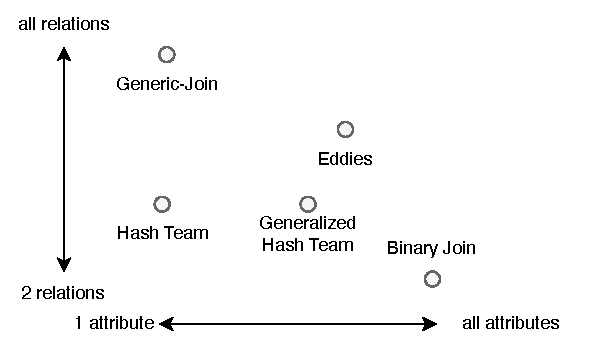
\includegraphics[width=0.55\linewidth]{free-join.pdf}
    \caption{Design space of join algorithms.}
    \label{fig:design-space}
\end{figure}

To explain these contributions we provide some context.
%
In this dissertation, we focus on algorithms based on hashing,
  and choose \GJ~\cite{DBLP:journals/sigmod/NgoRR13} as a representative of \WCOJ algorithms.
A crucial difference between \GJ and binary join lies 
  in the way they process each join operation. 
Binary join processes two relations at a time, 
  and joins on \emph{all attributes} 
  shared between these two relations. 
In contrast, \GJ processes one attribute at a time, 
  and joins \emph{all relations} that share that attribute.
This suggests a design space of join algorithms, 
  where each join operation may process any 
  number of attributes and relations.
Figure~\ref{fig:design-space} shows this design space
  which also covers classic multiway join algorithms 
  like Hash Team~\cite{DBLP:conf/vldb/GraefeBC98}, 
  Generalized Hash Team~\cite{DBLP:conf/vldb/KemperKW99}
  and Eddies~\cite{DBLP:conf/sigmod/HellersteinA00}.
Being able to join on any number of variables and relations
  frees us from the constraints of all existing algorithms 
  mentioned above. 
% } \yell{I suggest removing the boldface}

Our new framework, \FJ,
  covers the entire design space, 
  thereby generalizing and unifying existing algorithms.
The starting observation is that the execution of a {\em left-deep linear 
  binary join plan} (reviewed in Sec.~\ref{sec:background:fj}) is already very similar to \GJ.
While \GJ (also reviewed in Sec.~\ref{sec:background:fj}) is traditionally specified as a series of nested loops~\cite{DBLP:journals/sigmod/NgoRR13},
  the push-based model~\cite{DBLP:journals/pvldb/Neumann11,DBLP:journals/pvldb/KerstenLKNPB18} for executing a left-deep linear binary plan
  is also implemented, similarly, as nested loops.
% \rw{Should I add an example of the loop nest, or is that too much detail?}
% \ds{Not here, but please explain this point again in the technical
%   sections, and give an example there.}
The two algorithms also process each join operation similarly:
  each binary hash join iterates over tuples on one relation, 
  and for each tuple probes into the hash table of another relation;
  each loop level in \GJ iterates over the keys of a certain trie,
  and probes into several other tries for each key.
This inspired us to unify hash tables and hash tries into the same data structure, 
  and develop \FJ using iteration and probing as key operations.
This finer-grained view of join algorithms allows \FJ
  to generalize and unify existing algorithms,
  while precisely capturing each of them.

  \FJ takes as input an already optimized binary join plan, and
  converts it into a new kind of plan that we call a \FJ plan.  It
  then optimizes the \FJ plan, resulting in a plan that sits in
  between binary join and \GJ, combining the benefits of both.  On one
  hand \FJ fully exploits the design space in
  Figure~\ref{fig:design-space}.  On the other hand, by starting from
  an already optimized binary plan, \FJ takes advantage of existing
  cost-based optimizers; in our system we used binary plans produced by
  the optimizer of DuckDB~\cite{DBLP:conf/cidr/RaasveldtM20,DBLP:conf/vldb/Raasveldt22}.

Next, we address the main source of
  inefficiency in \GJ: the need to construct a trie on each relation
  in the query~\cite{DBLP:journals/pvldb/MhedhbiS19,DBLP:journals/pvldb/FreitagBSKN20}.  
In contrast,  a binary join plan needs to build a hash map only for each relation 
  on the right-hand side of a join,
  and simply iterates over the relation on the left.
As a result, a query optimizer commonly places the largest relation on the left
 to minimize the cost of hash building.
One simple optimization in \FJ is that we do not built a trie for
tables that are left children, mimicking the binary plans.
%
However, we go a step further, and introduce the {\em Column-Oriented
  Lazy Trie} (\COLT) data structure, which builds the inner subtries
  lazily, by creating each subtrie on demand.  
We note that this builds on an earlier idea
in~\cite{DBLP:journals/pvldb/FreitagBSKN20}.  As the name suggests,
\COLT adapts the lazy trie data structure
in~\cite{DBLP:journals/pvldb/FreitagBSKN20} to use a column-oriented
layout.  And unlike the original lazy trie which builds at least one
trie level per table, \COLT completely eliminates the cost of trie
building for left tables.


Finally, we describe a method for incorporating vectorized
  processing in \FJ, allowing it to collect multiple data values
  before entering the next iteration level.  
The standard \GJ processes one data value at a time, but, as is the
  case in traditional query engines, this leads to poor cache
  locality.  
Vectorized execution~\cite{DBLP:conf/icde/PadmanabhanAMJ01} was proposed for binary join
  to improve its locality by processing data values in batch.
By breaking down join operations into iterations and probes, 
  \FJ gives rise to a simple vectorized execution algorithm
  that breaks each iteration into chunks and groups together 
  batches of probes.
Our proposal is to our knowledge the first vectorized execution algorithm for \GJ.

We implemented \FJ as a standalone Rust library, and
compared it with two baselines:
  \begin{enumerate*}
    \item our own \GJ implementation in Rust, and
    \item the binary hash join implemented in
      DuckDB~\cite{DBLP:conf/cidr/RaasveldtM20,DBLP:conf/vldb/Raasveldt22},
      a state-of-the-art in-memory database.
    \end{enumerate*}
    %%%%%%%%%% No need for experimental details here, just some highlights
%%%   We conduct experiments on the popular Join Order
%%%   Benchmark~\cite{DBLP:journals/pvldb/LeisGMBK015} and the
%%%   LSQB~\cite{} benchmark.
  We found that, on acyclic queries, \FJ is up to \imdbmaxfjbj
  faster than binary join, and up to \imdbmaxfjgj faster than \GJ; on
  cyclic queries, \FJ is up to 15.45x faster than binary join, and up
  to 4.08x faster than \GJ.
  % \FJ also retains its advantage even when the optimizer chooses a poor plan.
%%%   We conduct additional experiments on
%%%   synthetic data for star and chain queries, as well as ablation
%%%   studies on the optimizations.  Finally, we compare \FJ and binary
%%%   hash join on their robustness against bad query plans.  Given a bad
%%%   query plan, \FJ runs up to \hjbad and \gjbad faster than binary join
%%%   and \GJ, respectively.

  While optimizers for binary plans have been developed and improved
  over decades~\cite{DBLP:conf/sigmod/SelingerACLP79}, little
  is known about optimizing \GJ.  A \GJ plan consists of a total order
  on its variables, and its run time depends on the choice of this
  order.  But since the theoretical analysis of \GJ guarantees worst
  case optimality for {\em any} variable order, it is a folklore
  belief that \GJ is more robust than binary join plans 
  when the optimizer makes a bad choice.
  To test the robustness of binary join, \GJ, and \FJ, 
  We also conducted experiments measuring their 
  performance when given a bad query plan.
  We found that \GJ is indeed the
  least sensitive, while \FJ, like binary joins, suffers more from the
  poor optimization choices of the optimizer, since both rely on a
  cost-based optimized plan.  However, \GJ starts from worse baseline
  than \FJ.  In other words, \FJ takes better advantage of a good
  plan, when available, than \GJ does.


  
In summary, we make the following contributions in this dissertation:
% \ds{Please reference the sections where these contributions are
%   described.  Currently the do NOT align with the contributions
%   mentioned earlier and discussed in the introduction.  This needs to
%   be fixed.}
% \rw{Fixed.}
\begin{enumerate}
  \item \FJ, a framework unifying existing join algorithms (Section~\ref{sec:free-join}).
  \item An algorithm to converting a binary plan into an
    optimized \FJ plan (Section~\ref{sec:bj-to-fj}).
  \item \COLT, a column-oriented lazy trie data structure (Section~\ref{sec:colt}).
  \item A vectorized execution algorithm for \FJ (Section~\ref{sec:vectorized-execution}).
  \item Experiments evaluating the algorithms and optimizations (Section~\ref{sec:eval}).
\end{enumerate}

\section{Background}\label{sec:background:fj}

This section defines basic concepts and reviews background on binary
join and \GJ.

\subsection{Basic Concepts}\label{sec:basic-concepts}

In previouse chapters we have used upper case variables for key values, 
 and reserved lower case variables for semiring values. 
As we do not deal with semirings in this chapter, 
 we will use lower case variables for key values to reduce clutter.
Recall from Section~\ref{sec:join} that a \emph{full conjunctive query} 
 has the following form:
%
\begin{align}
  Q(\bm x) \cd & R_1(\bm x_1), \ldots, R_m(\bm x_m). \label{eq:cq}
\end{align}
%
where each variable in a body atom $R_i({\bm x_i})$ also appears 
 in the head $R({\bm x})$.
We will assume that the query does not have {\em self-joins},
 meaning no two atoms share the same relation name.
This is without loss of generality: if two atoms have the same
relation name, then we simply rename one of them.  
Our system also supports selections, projections, and aggregation.  
We assume that the selections are pushed down to the base tables, thus the atom $R_i$
in~\eqref{eq:cq} may include a selection over a base table; in
particular, all variables in the atom $R_i(\bm x_i)$ are distinct.
Similarly, projections and aggregates are performed after the full
join, hence none of them is shown in~\eqref{eq:cq}.


\begin{ex} \label{ex:triangle} Consider the following SQL query:
\begin{lstlisting}[
    language=SQL,
    showspaces=false,
    basicstyle=\ttfamily\small,
    % numbers=left,
    % numberstyle=\tiny,
    commentstyle=\color{gray}
 ]
SELECT r.x, s.u, t.u
  FROM R as r, M as s, M as t -- schema: R(x,y), M(u,v,w)
 WHERE s.w > 30 AND t.v = t.w
   AND r.y = s.u AND s.v = t.u AND t.v = r.x
\end{lstlisting}
%
Then we denote by $S = \Pi_{uv}(\sigma_{w>30}(M))$ and $T =
\Pi_{uv}(\sigma_{v=w}(M))$, and write the query as:
$$Q_{\triangle}(x,y,z) \cd R(x, y), S(y,z), T(z, x).$$
%
We call this query the \emph{triangle query} over the relations $R$, $S$,
$T$.
\end{ex}

It is often convenient to view the conjunctive query~\eqref{eq:cq} as
a hypergraph.  The \emph{query hypergraph} of $Q$ consists of vertices
$\mathcal{V}$ and edges $\mathcal{E}$, where the set of nodes
$\mathcal{V}$ is the set of variables occurring in $Q$, and the set of
hyperedges $\mathcal{E}$ is the set of atoms in $Q$.  The hyperedge
associated to the atom $R(\bm x_i)$ is defined as the set consisting
of the nodes associated to the variables $\bm x_i$.  As standard, we
say that the query $Q$ is {\em acyclic} if its associated hypergraph
is $\alpha$-acyclic~\cite{DBLP:journals/jacm/Fagin83}


\subsection{Binary Join}\label{sec:binary-join}

The standard approach to computing a conjunctive query~\eqref{eq:cq} is
to compute one binary join at a time.  A {\em binary plan} is a binary
tree, where each internal node is a join operator $\Join$, and each
leaf node is one of the base tables (atoms) $R_i(\bm x_i)$ in the
query~\eqref{eq:cq}.  The plan is a \emph{left-deep linear plan}, or
simply left-deep plan, if the right child of every join is a leaf
node.  If the plan is not left-deep, then we call it \emph{bushy}.
For example, $(R \Join S) \Join (T \Join U)$ is a bushy plan, while
$((R \Join S) \Join T) \Join U$ is a left-deep plan.  We do not treat
specially right-deep or zig-zag plans, but simply consider them to be
bushy.

In this dissertation we consider only hash-joins, which are the most
common types of joins in database systems. 
The standard way to execute a bushy plan is to
decompose it into a series of left-deep linear plans.  Every join node
that is a right child becomes the root of a new subplan, which is
first evaluated, and its result materialized, before the parent join
can proceed.  As a consequence, every binary plan, bushy or not,
becomes a collection of left-deep plans. 
In our system we decompose bushy
plans exactly this way, and we will focus on left-deep linear
plans in the rest of this chapter.  For example, the bushy plan
$(R \Join S) \Join (T \Join U)$ is converted into two plans:
$P_1 = T \Join U$ and $P_2 = (R \Join S) \Join P_1$; both are
left-deep plans.

To reduce clutter, we represent a left-deep plan
$(\cdots ((R_1 \Join R_2) \Join R_3) \cdots \Join R_{m-1}) \Join R_m$
as $[R_1, R_2, \ldots, R_m]$.  Evaluation of a left-deep plan is done
using pipelining.  The engine iterates over each tuple in the
left-most base table $R_1$; each tuple is probed in $R_2$; each of the
matching tuple is further probed in $R_3$, etc.


\begin{figure}
  \begin{subfigure}[b]{0.5\linewidth}
\centering
\begin{tabular}{c}
\begin{lstlisting}
for (x, y) in R:
  s = S[y]?
  for (y, z) in s:
    t = T[x,z]?
    for (x, z) in t:
      output(x, y, z)
\end{lstlisting}
\end{tabular}
\caption{Binary join.}
\label{fig:background:binary-join}
  \end{subfigure}
% \hspace{2cm}
  \begin{subfigure}[b]{0.45\linewidth}
\centering
\begin{tabular}{c}
\begin{lstlisting}
for a in R.x $\cap$ T.x:
  r = R[a]; t = T[a]
  for b in r.y $\cap$ S.y:
    s = S[b]
    for c in s.z $\cap$ t.z:
      output(a, b, c)
\end{lstlisting}
\end{tabular}
    \caption{\GJ.}
    \label{fig:background:gj}
  \end{subfigure}
%  \Description[TODO]{TODO}
  \caption{Execution of binary join and \GJ for $Q_\triangle$.  The
    notation \lstinline|S[y]?| performs a lookup on $S$ with the key
    $y$, and continues to the enclosing loop if the lookup fails.
    Binary join iterates over {\em tuples}, \GJ iterates over {\em
      values}.}
\end{figure}

\begin{ex}
  A possible left-deep linear plan for $Q_\triangle$ is $[R, S, T]$,
  which represents $(R(x,y) \Join S(y,z)) \Join T(z,x)$.  To execute
  this plan, we first build a hash table for $S$ keyed on $y$, where
  each $Y$ maps to a vector of $(y,z)$ tuples, 
  % \yell{Remy: this is not
  %   correct.  The hash table contains tuples.  Think of a table that
  %   has 30 attributes $S(x_1,\ldots, x_{30})$.  If you join on
  %   $x_{12}$, you don't create a new tuple with 29 attributes, but
  %   store the whole tuple in the hash table.  Some systems actually
  %   store a pointer to the real tuple in the buffer pool.}
  and a hash table for $T$ keyed on $x$ and $z$, each mapped to a
  vector of $(x,z)$ tuples\footnote{When the relations are bags, then
    the hash table may contain duplicate tuples, or store separately
    the multiplicity.  We also note that the question what exactly to
    store in the hash table (e.g. copies of the tuples, or pointers to
    the tuple in the buffer pool) has been studied for a long time,
    see~\cite{DBLP:journals/csur/Graefe93}.}.  Then the execution
  proceeds as shown in Figure~\ref{fig:background:binary-join}.  For each
  tuple $(x, y)$ in $R$, we first probe into the hash table for $S$
  using $y$ to get a vector of $(y, z)$ tuples.  We then loop over
  each $(y, z)$ and probe into the hash table for $T$ using $x$ and
  $z$.  Each successful probe will return a vector of $(x, z)$ tuples,
  and we output the tuple $(x, y, z)$ for each $(x, z)$.
\end{ex}

\subsection{\GJ}\label{sec:background:gj}

\GJ was introduced in~\cite{DBLP:journals/sigmod/NgoRR13} and is the
simplest worst-case optimal join algorithm.  It is based on the
earlier Leapfrog Triejoin algorithm~\cite{DBLP:conf/icdt/Veldhuizen14}.
%
\GJ computes the query $Q$ in~\eqref{eq:cq} through a series of nested
loops, where each loop iterates over a variable (not a tuple).
Concretely, \GJ chooses arbitrarily a variable $x$, computes the
intersection of all $x$-columns of all relations containing $x$, and
for each value $a$ in this intersection it computes the residual query
$Q[a/x]$, where every relation $R$ that contains $x$ is replaced with
$\sigma_{x=a}(R)$.  In pseudocode:
%
\begin{lstlisting}
GJ: for a in $\bigcap \setof{\Pi_x(R_i)}{R_i \mbox{ contains } x}$
      compute Q[a/x]  \\ run GJ on Q with one fewer variable
\end{lstlisting}
%
If the query $Q$ has $k$ variables, then there are $k$ nested loops in
\GJ.  In the inner most loop, \GJ outputs the tuple of constants, one
from each iteration.\footnote{For bag semantics, it multiplies their
  multiplicities.}  We notice that a plan for \GJ consists of a total
order of the variables of the query, which we denote as
$[x_1, x_2, \ldots, x_k]$.  Assuming that the intersection above is
done optimally (see below), the algorithm is provably
worst-case-optimal, for any choice of the variable order.

\begin{ex}
  Fig.~\ref{fig:background:gj} illustrates the pseudocode for \GJ on the
  query $Q_\triangle$, using the variable order $[x,y,z]$.  We denoted
  $\Pi_x(R)$ by $R.x$, and denoted (with some abuse) $\sigma_{x=a}(R)$
  by $R[a]$.
\end{ex}


While binary joins use hash tables, an implementation of \GJ uses a
\emph{hash trie}, one for each relation in the query.  The hash-trie
is a tree, whose depth is equal to one plus the number of attributes
of the relation, and where each node is either an empty leaf
node,\footnote{For bag semantics, we store in the leaf the
  multiplicity of the tuple.} or a hash map mapping each atomic value
to another node.  We will call the \emph{level} of a node to be the
distance from the root, i.e. the root has level 0, its children level
1, etc.  The hash-trie completely represents the relation: every
root-to-leaf path corresponds precisely to one tuple in the relation.
\GJ uses the hash-trie as follows.  In order to compute
$\sigma_{x=a}(R)$, it simply probes the current hash table for the
value $x=a$, and returns the corresponding child.  To compute an
intersection $\Pi_x(R_1) \cap \Pi_x(R_2) \cap \cdots$, it selects the
trie with the fewest keys, say $R_1$, then iterates over every value
$a$ in the keys for $R_1$ and probes it in each of the hash-maps for
$R_2, R_3, \ldots$; this is a provably optimal algorithm for the
intersection.

\begin{ex}
  Consider the query $Q_\triangle$ and the \GJ plan $[x, y, z]$.  We
  first build a hash trie each for $R$, $S$, and $T$.  Each trie has
  three levels including the leaf.  Level 0 of $R$ is keyed on $x$,
  level 1 is keyed on $y$, level 2 contains empty leaf nodes, and
  similarly for $S$ and $T$.  Consider again the pseudocode in
  Figure~\ref{fig:background:gj}.  The first loop intersects level 0
  of the $R$-trie and the $T$-trie.  For each value $a$ in the
  intersection, we retrieve the corresponding children $R[a]$ and
  $T[a]$ respectively; these are at level 1.  The second loop
  intersects the hash map $R[a]$ (at level 1) with the level 0
  hash-map of $S$.  For each value $b$ in the intersection it
  retrieves the corresponding children (levels 2 and 1 respectively),
  and, finally, the innermost loop intersects the $S$- and $T$-hash
  maps (both at level 2), and outputs $(a,b,c)$ for each $c$ in the
  intersection.  So far we have assumed set semantics; if the
  relations have bag semantics, then we simply multiply the tuple
  multiplicities on the leaves (level 3).
\end{ex}

%%% The original \GJ algorithm was specified for set semantics,
%%% however~\cite{DBLP:journals/pvldb/FreitagBSKN20} showed the algorithm
%%% can be easily extended to bag semantics.  We therefore ignore the
%%% difference between the two semantics for the rest of this dissertation.

\subsection{Binary Join v.s. \GJ}
Binary join and \GJ each have their own advantages and disadvantages.
\GJ became popular because of its asymptotic performance guarantee:
\cite{DBLP:journals/sigmod/NgoRR13} proved the algorithm is
\emph{worst-case optimal} for \emph{any variable order}, in the sense
that its run time is bounded by the largest possible size of its
output, called AGM bound~\cite{DBLP:journals/siamcomp/AtseriasGM13}.
For example, \GJ executes $Q_\triangle$ in time
$\sqrt{|R|\cdot |S| \cdot |T|}$, which is $n^{3/2}$ when all relations
have size $n$; in contrast, a binary join plan can take $\Omega(n^2)$.
We note, however, that this formula does not include the preprocessing
time needed to construct the tries.  For example, if $T$ is
significantly larger than $R, S$, then the run time of \GJ is
$\ll |T|$, yet during preprocessing \GJ needs to read the entire
relation $T$.  On the other hand, binary join has been a staple of
database systems for decades.  The hash table data structure is
simpler than hash tries and is cheaper to build.  Techniques like
vectorized execution and column-oriented layout have also made binary
join practically efficient, but these optimizations have not been
adapted for \GJ.  Binary join plans are known to be very sensitive to
the choice of the optimizer: poor plans perform catastrophically
bad~\cite{DBLP:journals/pvldb/LeisGMBK015}.  In contrast, although the
runtime performance of \GJ does depend on the variable order, some
researchers believe that \GJ is less sensitive to poor variable
orders, in part because it is worst-case optimal.

\section{\FJ}\label{sec:free-join}

In this section we introduce the \FJ framework.
We start by presenting the Generalized Hash Trie (\GHT) which
 is the data structure used in \FJ (Section~\ref{sec:ght}).
Next we introduce the \FJ plan that specifies 
  how to execute a query with \FJ (Section~\ref{sec:fj-plan}).
Finally, we describe the \FJ algorithm, 
  which takes as input a collection of \GHTs 
  and a \FJ plan,
  and computes the query according to the plan (Section~\ref{sec:free-join-algorithm}).
  
We will show how each of the above components generalizes 
  and unifies the corresponding components in binary join 
  and \GJ: 
  the \GHT generalizes hash tables and hash tries,
  the \FJ plan generalizes binary plans and \GJ plans, and
  the \FJ algorithm generalizes binary join and \GJ.

\begin{figure}
\begin{subfigure}[b]{0.49\linewidth}
\begin{align*}
  Q_{\clubsuit}(x,a,b,c) \cd R(x,a),S(x,b),T(x,c)
\end{align*}
\begin{alignat*}{4}
  R & = \set{(x_0, a_0)} && \cup \{(x_1, a_i^l), (x_2, a_i^r &&) \mid i \in [1 \ldots n] \} \\
  S & = \set{(x_0, b_0)} && \cup \{(x_2, b_i^l), (x_3, b_i^r &&) \mid i \in [1 \ldots n] \} \\
  T & = \set{(x_0, c_0)} && \cup \{(x_3, c_i^l), (x_1, c_i^r &&) \mid i \in [1 \ldots n] \} 
  % R & = \set{(x_0, a_0)} \cup \bigcup_{i \in [1 \ldots n]} \set{(x_1, a_i^l), (x_2, a_i^r)} \\
  % S & = \set{(x_0, b_0)} \cup \bigcup_{i \in [1 \ldots n]} \set{(x_2, b_i^l), (x_3, b_i^r)} \\
  % T & = \set{(x_0, c_0)} \cup \bigcup_{i \in [1 \ldots n]} \set{(x_3, c_i^l), (x_1, c_i^r)} 
\end{alignat*}
\caption{$Q_\clubsuit$ and inputs.}
\label{fig:clover-query}
\end{subfigure}
\begin{subfigure}[b]{0.5\linewidth}
  \centering
  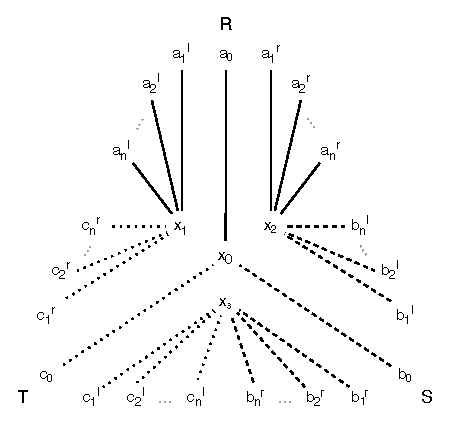
\includegraphics[width=0.8\linewidth]{sand-dollar.pdf}
  \caption{Visualization of the input relations.}
  \label{fig:clover-vis}
\end{subfigure}
\caption{(\ref{fig:clover-query}) the clover query $Q_\clubsuit$, and an input instance.
(\ref{fig:clover-vis}) visualization of the instance in
    Fig.~\ref{fig:clover-query}. The solid (top) edges form the relation
    \texttt{R}, the dashed (right) edges form the relation \texttt{S},
    and the dotted (left) edges form the relation \texttt{T}.  The
    relations join on the attribute in the center.  The only output
    tuple consists of the three edges in the center. }
\end{figure}

Throughout this section we will make use of the {\em clover query}
$Q_\clubsuit$ in Figure~\ref{fig:clover-query}.
Figure~\ref{fig:clover-vis} visualizes the input relations for this query.
Note that $Q_\clubsuit$ is
\emph{acyclic}.

\subsection{The Generalized Hash Trie}\label{sec:ght}

\begin{figure}
\begin{lstlisting}
interface GHT {
  # fields
  relation: String, vars: Vec<String>  
  # constructor
  fn new(name: String, schema: Vec<Vec<String>>) -> Self
  # methods
  fn iter() -> Iterator<Tuple>
  fn get(key: Tuple) -> Option<GHT> }
\end{lstlisting}
\caption{The \GHT interface.}
\label{fig:ght}
\end{figure}

To unify binary join and \GJ, 
  we first need to unify the data structures they work over.
We propose the Generalized Hash Trie 
  which generalizes both the hash table used in binary join 
  and the hash trie used in \GJ.

\begin{defn}[Generalized Hash Trie (\GHT)]
  A \GHT is a tree where each leaf is a vector of tuples, and
  each internal node is a hash map whose keys are tuples, and each key
  maps to a child node.
\end{defn}

We will reuse the terminology defined for tries, including
\emph{level}, \emph{node}, and \emph{leaf}, etc., for \GHTs.  We will
also use the terms \GHT and \emph{trie} interchangeably when the
context is clear.  The {\em schema} of a \GHT is the list
$[\bm y_0,\bm y_1, \ldots, \bm y_\ell]$ where $\bm y_k$ are the
attribute names of the key at level $k$. 

The hash trie used in \GJ is a \GHT where each key is a tuple of size one,
  and the last level stores empty vectors, each of which represents a leaf.
The hash table used in binary join is very similar to a \GHT with only two levels,
  where level 0 stores the keys and level 1 stores
  vectors of tuples.
A small difference is that, in the \GHT, the concatenation of 
  a tuple from level 0 with a tuple from level 1 forms a tuple in the relation, 
  whereas each whole tuple is stored directly in a hash table.
We will show in Section~\ref{sec:colt} how the \COLT data structure
  more faithfully captures the structure of a hash table.
Figure~\ref{fig:ght-examples} shows two examples of \GHTs.

We use \GHTs to represent relations,
  and attach metadata as well as access methods 
  to each \GHT, to be used by the \FJ algorithm.
The \GHT interface is shown in Figure~\ref{fig:ght}.
The \lstinline|relation| field stores the relation name.
A sub-trie inherits its name from its parent.
The \lstinline|vars| field stores parts of the relation's schema:
  if the trie is a vector of tuples, 
  \lstinline|vars| is the schema of each tuple;
  if the trie is a map, 
  \lstinline|vars| is the schema of each key.
The constructor method \lstinline|new| creates a new \GHT from the named relation, 
  where an $n$-th level trie has variables
  matching the $n$-th element of the \lstinline|schema| argument,
  and the values along each path from the root to a leaf of the \GHT 
  form a tuple in the relation.

\begin{ex}
  Both \GHTs in Figure~\ref{fig:ght-examples} represent relation $S$ from the
  clover query $Q_\clubsuit$ in Figure~\ref{fig:clover-query}.  The
  \GHT on the left (a hash trie) was created by calling the
  constructor method \lstinline|new| with the schema
  \lstinline|[[x],[b],[]]|, so the top-level trie has the schema
  \lstinline|[x]|, each second-level trie has the schema
  \lstinline|[b]|, and each third-level trie (a leaf) has the empty
  schema \lstinline|[]|.  The \GHT on the right (a hash table) was
  created by calling \lstinline|new| with the schema
  \lstinline|[[x],[b]]|.  It has only two levels, with schema
  \lstinline|[x]| and \lstinline|[b]|, respectively.  Note that each
  $b$ value in the hash trie is hashed and stored as a key, while the
  $b$ values in the hash table are simply stored in vectors.
\end{ex}

The methods \lstinline|iter| and \lstinline|get| 
  provide access to values stored in the trie.
If the trie is a map, 
  \lstinline|get(key)| returns the sub-trie mapped to \lstinline|key|,
  if any.
Calling \texttt{get} on a vector returns \lstinline|None|.
If the trie is a vector, 
  \lstinline|iter()|
  returns an iterator over the tuples in the vector;
  calling \texttt{iter} on a map 
  returns an iterator over the keys.

\begin{figure}
  \centering
  \begin{subfigure}[c]{0.3\linewidth}
  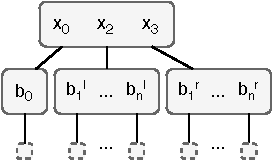
\includegraphics[width=\textwidth]{trie}
  \end{subfigure}\hspace{1.5cm}%
  \begin{subfigure}[c]{0.3\linewidth}
  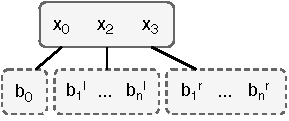
\includegraphics[width=\textwidth]{map}
  \end{subfigure} 
  \caption{
    Two \GHTs. The one on the left is also a hash trie, 
      and the one on the right is similar to a hash table.
    Each box with solid border stores hash keys, 
    and each box with dashed border is a vector of tuples.
    An empty box is an empty vector, representing a leaf.
  }
  \label{fig:ght-examples}
\end{figure}

\begin{ex}
  On the second \GHT in Figure~\ref{fig:ght-examples},
    calling \texttt{iter} returns an 
    iterator over the values $[x_0, x_2, x_3]$.
    Calling \texttt{get} with the key $x_2$ 
    returns the sub-trie which is the vector $[b_1^l, \ldots, b_n^l]$.
  Calling \texttt{iter} on this sub-trie
    returns an iterator over $[b_1^l, \ldots, b_n^l]$.
\end{ex}


\subsection{The \FJ plan}\label{sec:fj-plan}

% \ds{The section tile doesn't seem right.  What about ``The \FJ plan''}

A \FJ plan specifies how the \FJ algorithm should be executed.
It generalizes and unifies binary join plans and \GJ plans. 
Recall that a left-deep linear plan for binary join
  is a sequence of relations;
  it need not specify the join attributes, 
  since all shared attributes are joined.
In contrast, a \GJ plan is a sequence of variables;
  it need not specify the relations, 
  since all relations on each variable are joined.
A \FJ plan may join on any number of variables and relations at each step,
  and therefore needs to specify both explicitly.

  To help define the \FJ plan, we introduce two new concepts, called
  \emph{subatom} and \emph{partitioning}.  Fix the query $Q$ in
  Eq.~\eqref{eq:cq}:

\begin{defn}
  A \emph{subatom} of an atom $R_i(\bm x_i)$ is an expression
  $R_i(\bm y)$ where $\bm y$ is a subset of the variables $\bm x_i$.
  A \emph{partitioning} of the atom $R_i(\bm x_i)$ is a set of
  subatoms $R_i(\bm y_1), R_i(\bm y_2), \ldots$ such that
  $\bm y_1, \bm y_2, \ldots$ are a partition of $\bm x_i$.
\end{defn}

We now define the \FJ plan using these concepts.

\begin{defn}[\FJ Plan]
  Fix a conjunctive query $Q$.  A \FJ \emph{plan} is a list
  $[\phi_1, \ldots, \phi_m]$, where each $\phi_k$ is a list of
  subatoms of $Q$, called a {\em node}.  The nodes are required to
  {\em partition the query}, in the sense that, for every atom
  $R_i(\bm x_i)$ in the query, the set of all its subatoms occurring
  in all nodes must form a partitioning of $R_i(\bm x_i)$.  We denote
  by $vs(\phi_k)$ the set of variables in all subatoms of $\phi_k$.
  The variables \emph{available to} $\phi_k$ are all the variables of the
  preceding nodes:
%
$$avs(\phi_k) = \bigcup_{j < k} vs(\phi_j)$$
%
\end{defn}

%%% Since the partitioning of each atom into subatoms can be inferred 
%%%   from the sequence of nodes, we will omit the partitioning 
%%%   when specifying a \FJ plan.

We will define shortly a {\em valid plan}, but first we show an example.

%%% While a \GJ plan consists of total order of the variables, a \FJ plan
%%% defines only a partial order, if we set
%%% $vs(\Phi_i) < vs(\Phi_2) < \cdots$.


\begin{ex}\label{ex:fj-plan}
  The following is an \FJ plan for $Q_\clubsuit$:
\begin{align}
&  [[R(x, a), S(x)], [S(b), T(x)], [T(c)]]\label{eq:bj-plan}
\end{align}
%
To execute the first node we iterate over each tuple $(x, a)$ in $R$
and use $x$ to probe into $S$; for each successful probe we execute
the second node: we iterate over each $b$ in $S[x]$, then use
$x$ to probe into $T$; finally the third node iterates over $c$ in
$T[x]$.  The reader may notice that this corresponds precisely to the
left-deep plan $(R(x,a) \Join S(x,b))\Join T(x,c)$.
%
Another \FJ plan for $Q_\clubsuit$ is: 
%
\begin{align}
  [[R(x), S(x), T(x)], [R(a)], [S(b)], [T(c)]]\label{eq:gj-plan}
\end{align}
%
This plan corresponds to the \GJ plan $[x,a,b,c]$.  Intuitively, here
we start by intersecting $R.x \cap S.x \cap T.x$, then, for each $x$
in the intersection, we retrieve the values of $a$, $b$, and $c$ from
$R$, $S$, and $T$, and output their Cartesian product.
\end{ex}

% \begin{figure}
%   \begin{subfigure}[t]{0.4\linewidth}
%     \centering
%     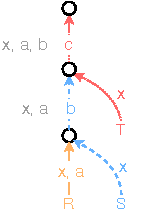
\includegraphics[height=35mm]{fj.pdf}
%     \caption{Plan in Eq.~\eqref{eq:bj-plan} (binary)}
%     \Description[TODO]{TODO}
%     \label{fig:bj-plan}
%   \end{subfigure}
%   \begin{subfigure}[t]{0.5\linewidth}
%     \centering
%     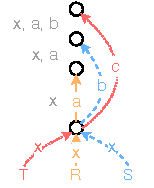
\includegraphics[height=32mm]{gj.pdf}
%     \caption{Plan in Eq.~\eqref{eq:gj-plan} (\GJ)}
%     \label{fig:gj-plan}
%   \end{subfigure}
%   \caption{Visualization of \FJ plans using notations from tensor
%     algebra~\cite{DBLP:journals/pacmpl/KjolstadKCLA17}.  Each circle
%     is a join node.  Arrows pointing to a node indicate the subatoms
%     in that node.  The same color and line style signify the same
%     relation. Grey text shows available variables.}
%   \label{fig:fj-plans}
% \end{figure}

% Readers familiar with tensor algebras may view \FJ as an
% \emph{iteration graph}~\cite{DBLP:journals/pacmpl/KjolstadKCLA17}, as
% shown in Figure~\ref{fig:fj-plans}.  We can ``read off'' the binary
% join plan $[R, S, T]$ from Figure~\ref{fig:bj-plan} by ignoring the
% variables.  Similarly, if we follow the variables in
% Figure~\ref{fig:gj-plan} bottom-up and ignore duplicates, we obtain the \GJ
% plan $[x, a, b, c]$.

Not all \FJ plans are valid, and only valid plans can be executed.  We
execute each \FJ node by iterating over one relation in that node, and
probe into the others.  Therefore, the values used in each probe must
be available, either from the same node or a previous one.

\begin{defn}
  A \FJ plan is \emph{valid} if for every node $\phi_k$ the following
  two properties hold.  (a) No two subatoms share the same relation,
  and (b) there is a subatom containing all variables in
  $vs(\phi_k) - avs(\phi_k)$.  We call such an subatom a \emph{cover}
  for $\phi_k$, and write $cover(\phi_k)$ for the set of covers.
\end{defn}

We will assume only valid plans in the rest of the paper.  To simplify
the presentation, in this section we assume that each node $\Phi_k$,
has {\em one} subatom designated as cover, and will always list it as
the first subatom in $\Phi_k$.  We will revisit this assumption in
Sec.~\ref{sec:optimization}, and allow for multiple covers.

%%% By this definition, every node must contain at least one subatom.  In
%%% addition, since we rename relations in a self-join as described in
%%% Section~\ref{sec:background}, a variable cannot appear in more than
%%% one subatom with the same relation name, and the same variable cannot
%%% appear more than once in the same subatom.

\begin{ex}
  Both plans in Example~\ref{ex:fj-plan} are valid.  The covers for
  the 3 nodes for Eq.~\eqref{eq:bj-plan} are $R(x, a)$, $S(b)$, and
  $T(c)$, respectively. For the plan in Eq.~\eqref{eq:gj-plan}, the
  covers for the 4 nodes are $R(x), R(a), S(b), T(c)$; for the first
  node we could have also chosen $S(x)$ or $T(x)$ as cover.
\end{ex}
 
% \ds{A few issues in the paragraph above and earlier.  You need to
%   define an atom, since this seems to be nonstandard: I assume you
%   mean that an atom consists of a relation name and a subset of the
%   variables.  The statement ``we do not allow self-joins'' raises
%   eyebrows; I don't think you mean that, please clarify.  The last
%   restriction (no atom contains the same variable twice) is OK, but
%   should be stated and explained in Sec.~\ref{sec:background}.}
% \rw{Will clarify in Backgroud.
%  For self-joins, we do allow them, but we rename the relation names to be different,
%  so that it looks like a join between different relations.
%  I'll also clarify this in Backgroud.  }
% \rw{Add because we rename them.}
% \rw{Use partial atom instead of an atom.}

% \ds{Before the next example add a brief explanation why the plans in
%   Ex.~\ref{ex:fj-plan} are valid.}
\begin{ex}
  An example of an \emph{invalid} plan for the clover query has one
  single node containing all relations and variables:
%
  $$[[R(x, a), S(x, b), T(x, c)]]$$
%
  Intuitively, we cannot execute it: if we iterate over, say $R$, then
  we bind two variables $x$ and $a$, but to lookup $S$ we
  need the key $(x,b)$.
\end{ex}

% \rw{We partition each atom to subatoms, 
% and define a plan for the query.
% }
% \begin{defn}
%   Given a \FJ plan $[\phi_1, \ldots, \phi_n]$, where 
% $\phi_i = \set{R_1(\overline{x_{i,1}}), \ldots, R_m(\overline{x_{i,m}})}$,
% \FJ computes the query:
% $$Q(*) \cd R_1(\overline{x_{1,1}}, \ldots, \overline{x_{n,1}}), \ldots, R_m(\overline{x_{1,m}}, \ldots, \overline{x_{n,m}}).$$
% That is, for each relation, we concatenate all its variables in the plan in order to form the query. 
% \end{defn}

% \begin{ex}
%   Both plans in Eq.~\eqref{eq:bj-plan} and Eq.~\eqref{eq:gj-plan} 
%   compute the clover query $Q(x,a,b,c) \cd R(x,a), S(x,b), T(x,c).$
% \end{ex}

% \ds{Add a definition saying ``Given a plan $P$, the query computed by
%   $P$ is $\ldots$'' Then illustrate this defintion with
%   Example~\ref{ex:fj-plan} and the example below.}

% \begin{ex}
%   The plan $[\phi=\set{R(), S(), T()}]$ is valid and computes the three-way 
%   Cartesian product of the relations (it does not compute the clover query).
%   The plan is vacuously valid because $vs(\phi) = \emptyset$.
%   Both plans in Eq.~\eqref{eq:bj-plan} and Eq.~\eqref{eq:gj-plan} are also valid.
% \end{ex}

% \ds{Equation numbers should be referred to using $\backslash$eqref
%   instead of $\backslash$ref.  I changed them in this file.}

\subsection{Execution of the \FJ Plan}\label{sec:free-join-algorithm}

% \ds{Suggestion: I would call this section ``Execution of the \FJ
%   Plan'' to better connect it to the previous section.}

The execution of a \FJ plan has two phases: the build phase and the
join phase.  The build phase constructs the \GHTs for the relations in
the query, by calling the constructor method \lstinline|new| on each
relation with the appropriate schema.  The join phase works over the
\GHTs to compute the join of the relations.

% fn ght_schema(relation, plan):
%   schema = []
%   for node in plan:
%     for atom in node:
%       if atom.relation == relation:
%         schema.append(atom.variables)
%   return schema 

\begin{figure}
  \begin{lstlisting}[
    commentstyle=\color{gray},
    escapeinside={(*}{*)},
    ]
fn join(all_tries, plan, tuple):
  if plan == []:
    output(tuple) (* \label{lst:output} *)
  else:
    tries = [ t $\in$ all_tries | t.relation $\in$ plan[0] ] (* \label{lst:select} *)
    # iterate over the cover
    @outer for t in tries[0].iter(): (* \label{lst:outer} *)
      subtries = [ iter_r.get(t) ] (* \label{lst:inner} *)
      tup = tuple + t
      # probe into other tries
      for trie in tries[1..]:     
        key = tup[trie.vars] (* \label{lst:key} *)
        subtrie = trie.get(key)
        if subtrie == None: continue @outer
        subtries.push(subtrie) (* \label{lst:inner-end} *)
      new_tries = all_tries[tries $\mapsto$ subtries] (* \label{lst:tuple} *)
      join(new_tries, plan[1:], tup) (* \label{lst:join} *)
\end{lstlisting}
  \caption{The \FJ algorithm.}
  \label{fig:fj-algo}
\end{figure}

\subsubsection*{Build Phase}
The build phase constructs a \GHT for each relation (atom)
$R_i(\bm x_i)$, as follows.  If the plan partitions the atom into the
subatoms $R_i(\bm y_0), R_i(\bm y_1), \ldots, R_i(\bm y_{\ell-1})$,
then the schema of its \GHT is the list
$[\bm y_0, \bm y_1, \ldots, \bm y_{\ell-1}, []]$.  Recall that the
last level of a \GHT is a vector instead of a hash map. As an
optimization, if the last subatom $R_i(\bm y_{\ell-1})$ is the cover
of its node, then we drop the last $[]$ from the schema, in other
words, we construct a vector for the $\bm y_{\ell-1}$.  After
computing the schema for each relation, we call the constructor method
\lstinline|new| on each relation and its computed schema to build the
\GHTs.

\begin{ex}
  Consider the plan in Eq.~\eqref{eq:bj-plan} for the clover query
  $Q_\clubsuit$.  The \GHT schemas for $R$, $S$, and $T$ are
  $[[x, a]]$, $[[x], [b]]$, and $[[x], [c]]$ respectively.  Thus, $R$
  is a flat vector of tuples, and each of $S$ and $T$ is a hash map of
  vectors of values.  Consider now the triangle query $Q_{\triangle}$
  and the plan $[[R(x,y),S(y),T(x)],[S(z),T(z)]]$.  The \GHT
  schemas for $R, S, T$ are $[[x,y]]$, $[[y],[z]]$, and $[[x],[z],[]]$:
  in other words $R$ is stored as a vector, $S$ is a hash-map of
  vectors, and $T$ is a hash-map of hash-maps of vectors.
\end{ex}

\subsubsection*{Join Phase}
The pseudo-code for the \FJ algorithm is shown in Figure~\ref{fig:fj-algo}.
The \lstinline|join| method takes as input the \GHTs, the \FJ plan, 
  and the current tuple initialized to be empty.
If the plan is empty, we output the tuple (line~\ref{lst:output}).
Otherwise, we work on the first node in the plan
  and intersect relevant tries (line~\ref{lst:select}).
We iterate over tuples in the covering relation, 
  which is the first trie in the node (line~\ref{lst:outer}).
%
% First we pick the trie to iterate over (line~\ref{lst:iter}).
% If any trie is a vector, we iterate over it.
% % \dan{I think it's clearer if you always iterate over the first
% %   subatom, which is the cover of the node.  We just need to make sure
% %   that this subatom is a vector, when that's possible.}
% % For now, we assume for each join node, at most one trie is a vector.
% % %
% % \yell{At this point there is nothing left to assume.  The \GHT is well
% %   defined, and only its last level is a vector, and the \GHT schema
% %   for a plan is well defined.  Everything is well defined.}
% % %
% We will relax this assumption in Section~\ref{sec:colt}.
% If all tries are hash maps, we iterate over the one with the fewest keys.
% After picking the trie to iterate over, 
%   we sort the other tries by some estimated cost to probe into them (line~\ref{lst:probe}).
% For example, we can probe into the smaller trie first, 
%   since it is likely to be selective, and may fit into the cache.
%
% In the outer for loop (line~\ref{lst:outer})
%   we iterate over each tuple \lstinline|t| in the trie we have picked.
Then, we use values from \lstinline|t| 
  and the \lstinline|tuple| argument
  as keys to probe into the other tries 
  (line~\ref{lst:inner}-\ref{lst:inner-end}).
To construct a key for a certain trie, 
  we find the values mapped from the trie's schema variables
  in \lstinline|t| and \lstinline|tuple| (line~\ref{lst:key}).
If any probe fails, we continue to the next tuple in the outer loop.
If all probes succeed, we replace the original tries with the 
  subtries returned by the probes,
  and recursively call \lstinline|join| 
  on the new tries and the rest of the plan (line~\ref{lst:tuple}-\ref{lst:join}).

The recursive definition may obscure the essence of the \FJ algorithm,
  so we provide some examples where we unroll the recursion.
We introduce some convenient syntax to simplify the presentation.
We write \lstinline|for (x,y,...) in T:| 
  to introduce a for-loop iterating over \lstinline|T|, 
  binding the values of each tuple in \lstinline|T.iter()| 
  to the variables \lstinline|x,y,...|.
We write \lstinline|r = R[t]?| to bind the result of 
  \lstinline|R.get(t)| to \lstinline|r|;
  if the lookup fails, we continue to the next iteration of the 
  enclosing loop.
In other words, \texttt{r = R[t]?} is equivalent to:
%
\begin{lstlisting}
r = R.get(t); if r.is_none(): continue
\end{lstlisting}

\begin{figure*}
  \begin{subfigure}[b]{0.3\linewidth}
\begin{lstlisting}[escapeinside={(*}{*)}]
R = GHT("R",[["x","a"]])
S = GHT("S",[["x"],["b"]])
T = GHT("T",[["x"],["c"]])
for (x, a) in R:
  s = S[x]?
  for b in s:
   (* \underline{t = T[x]?} *)
    for c in t:
      output(x, a, b, c)
\end{lstlisting}
    \caption{Binary \FJ.}
    \label{fig:bj-loop}
  \end{subfigure}
\hspace{1.5em}
  \begin{subfigure}[b]{0.3\linewidth}
    \centering
\begin{lstlisting}[
    escapeinside={(*}{*)}
]
# same as the left
# ...
# ...
for (x, a) in R:
  s = S[x]?
 (* \underline{t = T[x]?} *)
  for b in s:
    for c in t:
      output(x, a, b, c)
\end{lstlisting}
    \caption{Factorized \FJ.}
    \label{fig:factorized-loop}
  \end{subfigure}
  \hspace{.5em}
  \begin{subfigure}[b]{0.3\linewidth}
    \centering
\begin{lstlisting}
R = GHT("R",[["x"],["a"]])
# same as the left
# ...
for x in R:
  r=R[x]?; s=S[x]?; t=T[x]?
  for a in r:
    for b in s:
      for c in t:
        output(x, a, b, c)
\end{lstlisting}
    \caption{Generic \FJ.}
    \label{fig:gj-loop}
  \end{subfigure}
  \caption{Execution of \FJ for the clover query.}
\end{figure*}

\begin{ex}\label{ex:binary-free-join}
  Consider the plan in Eq.~\eqref{eq:bj-plan} for the clover query $Q_\clubsuit$.
  Figure~\ref{fig:bj-loop} shows its execution; ignore the underlined
  instruction for now.
%%%   Here we have omitted all ``setup'' code, 
%%%     showing only the nested loops performing iteration and lookup.
  In the build phase, 
    we construct a flat vector for $R$ and a hash table for each of $S$ and $T$.
  In the join phase, for the  node $[R(x, a), S(x)]$  we 
   iterate over $R$ and probe into $S$, while for the second node $[S(b), T(x)]$,
    we iterate over the second level of $S$ and probe into $T$.
  Finally, the third loop iterates over the second level of $T$ and outputs the result.
\end{ex}

\begin{ex}\label{ex:generic-free-join}
  Consider now the plan in Eq.~\eqref{eq:gj-plan} for  $Q_\clubsuit$.
  Its execution is shown in Figure~\ref{fig:gj-loop}.
  We construct  hash tables for $R$, $S$, and $T$, keyed on $x$.
  The first loop level intersects the three relations on $x$, 
    and subsequent loop levels take the Cartesian product of the relations on $a$, $b$, and $c$.
\end{ex}

Note that Fig.~\ref{fig:bj-loop}
  follows the execution of binary hash join with the plan $[R, S, T]$,
  whereas Fig.~\ref{fig:gj-loop} follows the execution of \GJ
   with the plan $[x, a, b, c]$.  We will describe
   Fig.~\ref{fig:factorized-loop} later.

\subsection{Discussion}

\FJ plans generalize both traditional binary plans and \GJ.  
% We will describe in the next section a simple optimization that allows us to
% cover the full spectrum in Fig.~\ref{fig:design-space}.  
One
limitation so far is our assumption that the cover is chosen at
optimization time.  This was convenient for us to illustrate how
to avoid constructing some hash maps, by storing the last level of a
\GHT as vector, when it corresponds to a cover.  In contrast, \GJ
computes the intersection $R_1.x\cap R_2.x\cap \cdots$ by iterating
over the smallest set, hence it chooses the ``cover'' at run time.  We
will address this in the next section by describing \COLT, a data
structure that constructs the \GHT lazily, at run time, allowing us to
choose the cover during the {\em join phase}.

\section{Optimizing the \FJ Plan}

\label{sec:optimization}

In the previous section we have introduced \FJ plans and their associated
data structures, the \GHTs.  We have seen that a \FJ plan is capable
of covering the entire design space in Fig.~\ref{fig:design-space},
from traditional join plans to \GJ.  In this section we describe how
to build, optimize, and speedup the execution of a \FJ plan.  We start
from a conventional binary plan produced by a query optimizer, and convert
it into an optimized \FJ plan (Section~\ref{sec:bj-to-fj}). Next, we
introduce the \COLT data structure to greatly reduce the cost of
building the hash tries (Section~\ref{sec:colt}).  We present a simple
vectorized execution algorithm for \FJ
(Section~\ref{sec:vectorized-execution}), and finally, we discuss how
\FJ relates to \GJ (Section~\ref{sec:fj-gj-multijoin}).

%%% In the previous section we have described how \FJ can simulate either binary
%%% join or \GJ, by simulating their data structures, query plans, and execution
%%% algorithms.  This allows \FJ to match the performance of either binary join or
%%% \GJ, if we simply instantiate \FJ to be the same as either algorithm. In this
%%% section we describe three key techniques that improve \FJ's performance
%%% beyond that of binary join and \GJ. First, we describe how to convert a binary
%%% plan into an efficient \FJ plan (Section~\ref{sec:bj-to-fj}). Next, we
%%% introduce the \COLT data structure to greatly reduce the cost of building
%%% the hash tries (Section~\ref{sec:colt}).  Then we present a simple
%%% vectorized execution algorithm for \FJ that improves cache locality
%%% (Section~\ref{sec:vectorized-execution}).  Finally, we conclude this section
%%% by discussing how \FJ relates to \GJ and other multiway join algorithms (Section~\ref{sec:fj-gj-multijoin}).

\subsection{Building and Optimizing a \FJ Plan}\label{sec:bj-to-fj}

Our system starts from an optimized binary plan produced by a
traditional cost-based optimizer; in particular, we use DuckDB's
optimizer~\cite{DBLP:conf/cidr/RaasveldtM20,DBLP:conf/vldb/Raasveldt22}. We
decompose a bushy plan into a set of left-deep plans, as described in
Sec.~\ref{sec:background:fj}, then convert each left-deep plan into an
equivalent \FJ plan.  Finally, we optimize the converted \FJ plan,
resulting in a plan that can be anywhere between a left-deep plan or a
\GJ plan.

% fn gj2fj(gj_plan):
%   fj_plan = []
%   for x in gj_plan:
%     node = { r(x) | r $\in$ relations, x $\in$ r.schema }
%     fj_plan.push(node)
%   return fj_plan

\begin{figure}
  \begin{lstlisting}
fn binary2fj(bin_plan):
  fj_plan = []; r = bin_plan[0]
  $\phi_0$ = [ r(r.schema) ]; $\phi$ = $\phi_0$ # iterate over left relation
  for s in bin_plan[1:]:
    $\phi$.push(s(s.schema $\cap$ $avs(\phi)$)) # probe w/ available vars
    fj_plan.push($\phi$)
    $\phi$ = [ s(s.schema - $avs(\phi)$) ] # iterate over probe result
  fj_plan.push($\phi$)
  return fj_plan
\end{lstlisting}
  \caption{Translating a binary plans to a \FJ plan.}
  \label{fig:bj2fj}
\end{figure}

The conversion from a binary plan to an equivalent \FJ plan is done by the function
\lstinline|binary2fj| in Figure~\ref{fig:bj2fj}.  We begin by adding the full atom of the left
relation as the first subatom in the first \FJ plan node.  Then we iterate over
the remaining relations in the binary join plan.  For each relation, we add a
subatom whose variables are the intersection of the relation's schema with the
available variables at the current \FJ plan node. Then we create a new join
node, adding to it the relation with the remaining variables.  

\begin{ex}
  The binary plan $[R, S, T]$ for the clover query $Q_\clubsuit$ is
  converted into the \FJ plan shown in Eq.~\eqref{eq:bj-plan}.  For
  another example, consider a chain query:
$$Q \cd R(x, y), S(y, z), T(z, u), W(u, v).$$
The left-deep plan $[R, S, T, W]$ is converted into:
$$[[R(x, y), S(y)], [S(z), T(z)], [T(u), W(u)], [W(v)]]$$
\end{ex}

So far the algorithm in Figure~\ref{fig:bj2fj} produces a \FJ plan
that is equivalent to the left-deep plan.  Next, we
optimize the \FJ plan. The main idea behind our optimization is to
bring the query plan closer to \GJ, without sacrificing the benefits
of binary join.

For intuition, let us revisit the clover query $Q_\clubsuit$, and its
execution depicted in Fig.~\ref{fig:bj-loop} (as explained in
Example~\ref{ex:binary-free-join}).  Consider the input shown in
Fig.~\ref{fig:clover-vis}.  Both relations $R$ and $S$ are skewed on
the value $x_2$, and their join will produce $n^2$ tuples, namely
$\setof{(x_2, a_i, b_j)}{i, j \in [1..n]}$.  This means the body of
the second loop in Figure~\ref{fig:bj-loop} is executed $n^2$ times.
However, the $n^2$ tuples are only to be discarded by the join with
$T$ which does not contain $x_2$.

There is a simple fix to the inefficiency: we can pull the underlined
lookup on $T$ in Figure~\ref{fig:bj-loop} out of the loop over $s$ to
filter out redundant tuples early.  This results in the nested loops
in Figure~\ref{fig:factorized-loop} which runs in $O(n)$ time, because
the two lookups in the first loop already filter the result to a
single tuple.  At the logical level, we convert the first \FJ plan
into the second \FJ plan:
  %
  \begin{align*}
&\mbox{Naive plan (Eq.~\eqref{eq:bj-plan}):}&& [[R(x, a), S(x)], [S(b), T(x)], [T(c)]]\\
&\mbox{Optimized plan:} && [[R(x, a), S(x), T(x)], [S(b)], [T(c)]]
  \end{align*}
  %
  While this is closer to the \GJ in Figure~\ref{fig:gj-loop}, it
  differs in that it still uses the same \GHTs built for original
  plan, without the need for an additional hash table for $R$.

\begin{figure}
  \begin{lstlisting}
fn factor(plan):
  @outer: for i in [1..n-1].reverse():
    $\phi$ = plan[i]; $\phi'$ = plan[i-1]
    for $\alpha$ in $\phi$:
      if $\alpha$.vars $\subseteq avs(\phi) \wedge \alpha$.relation $\notin \phi':$
        $\phi$.remove($\alpha$); $\phi'$.push($\alpha$)
      else: continue @outer
\end{lstlisting}
  \caption{Factorizing a \FJ plan.}
  \label{fig:factorize-plan}
\end{figure}

More generally, we will optimize a \FJ plan by \emph{factoring out}
lookups, i.e. by moving a subatom from a node $\Phi_i$ to the node
$\Phi_{i-1}$.  In doing so we must ensure that the plan is still
valid, and also avoid accidental slowdowns.  For example, we cannot
factor the lookups on $S$ and $T$ beyond the outermost loop, because
that loop binds the variable $x$ used in the lookups.

The optimization algorithm for \FJ plans is shown in
Figure~\ref{fig:factorize-plan}. We traverse the plan in reverse order
visiting each node. For each node, if there is an atom whose variables
are all available before that node, and if the previous node does not
contain an atom of the same relation, we move the atom to the previous
node. These two checks ensure the factored plan remains valid.  The
last line in the algorithm ensures we factor lookups
\emph{conservatively}. That is, we factor out a lookup only if all
previous lookups in the same node have also been factored out. Doing
so respects the lookup ordering given by the original cost-based
optimizer, since scrambling this ordering may inadvertently slow down
the query. It should be clear that factoring out any lookup will always improve
performance.


%%%%%  the ideas in this example are already included earlier, so I
%%%%%  commented it out
%%% \begin{ex}
%%%   Given the \FJ plan in Eq.~\eqref{eq:bj-plan},
%%%   the algorithm in Figure~\ref{fig:factorize-plan} returns the plan 
%%%   $[[R(x, a), S(x), T(x)], [S(b)], [T(c)]]$. 
%%%   Figure~\ref{fig:bj-loop} shows the execution of the original plan, 
%%%   and Figure~\ref{fig:factorized-loop} shows the execution of the optimized plan.
%%% \end{ex}


\subsection{\COLT: Column-Oriented Lazy Trie}\label{sec:colt}

The original \GJ algorithm builds a hash trie for each input relation.
A left-deep plan avoids building a hash table on the left most
relation, since it only needs to iterate over it, and this is an
important optimization, since the left most relation is often the
largest one.  Building a subtrie can also be wasteful when that
subtrie's parent is pruned away by an earlier join, in which case the
subtrie will never be used.  To address that, we describe here how to
build the tries \emph{lazily}: we only build the trie for a
(sub-)relation at runtime, if and when we need to perform a lookup, or
need to iterate over a prefix of its tuples.  This idea leads to our
new data structure called Column-Oriented Lazy Trie, or \COLT for
short.  In our system  the raw data is stored column-wise, in main
memory, and each column is stored as a vector, as standard in
column-oriented databases~\cite{DBLP:journals/ftdb/AbadiBHIM13}.
%
\begin{defn}
  A \emph{\COLT} is a tree where each leaf is a vector of offsets into
  the base relation, and each internal node is a hash map mapping a
  tuple to a child node.
\end{defn}


\begin{figure}
  \centering
  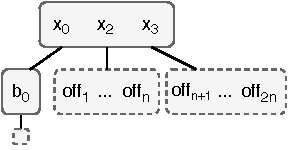
\includegraphics{colt.pdf}
  \caption{A \COLT for the relation $S$ in
    Fig.~\ref{fig:clover-query}. Each off$_i$ is an integer
    representing an offset into the table $S$.}
  \label{fig:colt}
\end{figure}

A \COLT tree need not be balanced, and there can be both hash maps and
vectors at the same tree level.  Fig.~\ref{fig:colt}
illustrates a \COLT tree for the instance $S$ of the clover query
$Q_\clubsuit$.

%%% \begin{ex}\label{ex:colt}
%%%   Recall the relation $S$ for the clover query $Q_\clubsuit$, 
%%%   whose \GHTs are shown in Figure~\ref{fig:ght-examples}.
%%%   Figure~\ref{fig:colt} shows a \COLT for $S$.
%%% \end{ex}


\begin{figure}
  \begin{lstlisting}
struct COLT {
  relation, schema, vars, 
  data = Map(HashMap<Tuple, COLT>) | Vec<Vec<u64>> }

impl GHT for COLT:
  fn new(relation, schema):
    COLT { relation, schema, schema[0],
           data = [ 0, 1, ..., relation.len - 1 ] }

  fn iter():
    match self.data:
      Map(m) => m.keys().iter(),
      Vec(v) => 
          if is_suffix(self.vars, relation.schema):
            v.map(|i| cols = self.relation[self.vars];
                      cols.map(|c| c[i]) )
          else: self.force(); self.iter()

  fn get(key): self.force(); self.get_map.get(key)

  fn force():
    match self.data:
      Map(m) => {} # already forced, do nothing
      Vec(v) => 
        map = new()
        for i in v:
          cols = self.relation[self.vars]
          k = cols.map(|col| col[i])
          if map[k] is None: # make a new, empty COLT
            map[k] = COLT { relation: self.relation, 
                            schema: self.schema[1..], 
                            data: [] }
          map[k].data.push(i)
        self.data = Map(map)
\end{lstlisting}
  \caption{The \COLT data structure.}
  \label{fig:colt-impl}
\end{figure}

% \ds{I did not understand the rest of this section.  What is needed:
%   (a) explain how the raw data is stored.  For example, how is a
%   relation $R(x,y,z)$ stored: row-wise? column-wise? sorted? (b) where
%   are the indices pointing to?  For example, if I construct the first
%   level of $R(x,y,z)$, then for each value of $x$ I have a set of
%   indices: where are these indices pointing to?}
% \rw{I added an example to explain this.}

\COLT Implements the \GHT interface in Figure~\ref{fig:ght}, and its
implementation is shown in Figure~\ref{fig:colt-impl}. As before,
\COLT stores a reference to the relation it represents, as well as the
\GHT schema computed from the plan.
%%% Recall the $i$-th element of the schema contains the variables at
%%% the $i$-th level of the trie.  For a (sub-)\COLT at level $k$,
%%% \lstinline|vars| is the same as the $k$-th element of the
%%% schema. the $0$-th element of the schema.
Consider a relation with $n$ tuples.  The \COLT tree is initialized
with a single node consisting of the vector $[0, \ldots, n-1]$,
i.e. one offset to each tuple.  
\COLT
implements the \lstinline|get| and \lstinline|iter| methods lazily.  
When
\lstinline|get| is called, we check if the current node is a hash
map or a vector.  In the first case, we simply perform a lookup in the
map.  In the second case, we first replace the current vector with a
hash map, whose children are vectors of offsets.  Notice that this
requires iterating over the current vector of offsets, accessing the
tuple in the base table, inserting the key in the hash map, and
inserting the offset in the corresponding child.  Consider now a call
to \lstinline|iter|.  If the current node is a hash map, then we
return an iterator over it.  If it is a vector, then we check if it is
a suffix of the relation schema: if yes, then we simply iterate over
that vector (and access the tuples via their offsets), otherwise we
first materialize the current hash map as explained above, and return
an iterator over the hash map.

As a simple but effective optimization, we do not initialize the \COLT
tree to the single node $[0,1,\ldots,n-1]$, but instead iterate
directly over the base table, if required.  If no \lstinline|get|
is performed on this table, then we have completely eliminated the
cost of building any auxiliary structure on this table.  Thus, the \FJ
plan can be equivalent to a left-deep plan that avoids building a hash
table on the left-most relation.  \COLT is also closer to the structure of
traditional hash tables, which, in some implementations, map a key to
a vector of pointers to tuples.
%
%%% Note that the \COLT for each relation of size $n$ is always initialized to be the 
%%%   vector $[0, \ldots, n-1]$.
%%% Since we can only iterate over this vector, 
%%%   we did not have to materialize it in the first place.
%%% Instead, we can simply loop over the tuples in the original relation 
%%%   when \lstinline|iter| is called.
%%% This means when the \FJ plan is equivalent to a binary plan, 
%%%   we completely eliminate the cost of trie building for the left relation, 
%%%   recovering the behavior of binary join.
%
%%% \COLT also captures the structure of hash tables more closely than
%%% \GHTs.  Recall that a hash table maps each key to an entire tuple in
%%% the relation.  Equivalently, we can also map the key to the row index
%%% of the tuple.  But that is precisely a \COLT whose first level is
%%% materialized.

\begin{ex}\label{ex:colt-clover}
Consider an extension of the clover query $Q_\clubsuit$:
\begin{align*}
  Q(x, a, b, c) \cd R(x,a), S(x,b), T(x, c), \underline{U(b)}.
\end{align*}
  % 
%   \begin{lstlisting}[
%     language=SQL,
%     showspaces=false,
%     basicstyle=\ttfamily\small,
%     commentstyle=\color{gray},
%     escapeinside={(*}{*)},
%  ]
% SELECT * FROM R,S,T,U -- schema: R(x,a),S(x,b),T(x,c),U(b)
%  WHERE R.x = S.x AND S.x = T.x AND T.x = R.x AND (*\underline{S.b = U.b}*)
% \end{lstlisting}
%
\GJ builds a 2-level hash trie for each of $R$, $S$, and $T$, as well
as a 1-level hash trie for $U$.  Consider the \FJ plan
$[[R(x,a),S(x),T(x)],[U(b),S(b)],[T(c)]]$.  \FJ executes the first
node of the plan by iterating over $R$ directly, without constructing
any auxiliary structure. For each tuple $(x, a)$ in $R$, it looks up
$x$ in $S$ and $T$.  Upon the first lookup, \COLT builds the first
level of the \GHT for $S$ and $T$, i.e. a hash map indexed by the $x$
values.  Assuming the database instance for $R,S,T$ shown in
Fig.~\ref{fig:clover-query}, the result of $R.x \cap S.x \cap T.x$ has
only one value, $x_0$, thus, $\FJ$ executes the second node for only
one value $x_0$.  Here it needs to intersect $U(b)$ and $S(b)$.
Assume for the moment that \FJ chooses $U(b)$ to be the cover, on the
first lookup in $S$, \COLT will expand the second level, arriving at
Figure~\ref{fig:colt}: notice that all other $b$ values in $S$ will
never be inserted in the hash table.  More realistically, \FJ follows
the principle in \GJ and chooses $S(b)$ as cover, because it is the
smallest: it builds a hash map for $U$, but none for the 2nd level of
$S$.
\end{ex}

The example highlights a divergence between \GJ and traditional plans.
To intersect $R_1.x \cap R_2.x \cap \ldots$, \GJ choose to iterate
over the smallest relation, which results in the best runtime {\em
  ignoring} the build time.  A traditional join plan will iterate over
the largest relation, because then it needs to build hash tables only
on the smaller relations.  Currently, we follow \GJ, and plan to
explore alternatives in the future.

% \ds{Remy please check the example and the discussion}


% \ds{The example doesn't help.  Once we have identified the single
%   value $b_0$, we only need to look it up in $U(b)$.  But since we
%   haven't constructed anything for $U$ yet, this requires a full scan
%   of $U$.  This is modestly better than scanning $U$ to create a
%   hash-table, but I don't see how this savings generalizes.  If the
%   previous joins return the values $b_0, b_1, b_2, \ldots$, then how
%   can we look them up in $U$ more efficiently than computing a hash
%   table on $U$?}
% \rw{Scanning $U$ while probing into the small trie is much faster than 
% building a hash table for $U$, since the latter needs to allocate memory.
% But the main point is not about $U$, but rather we avoid building a large 
% part of the second level of $S$.  }

\subsection{Vectorized Execution}\label{sec:vectorized-execution}
The \FJ algorithm as presented in Figure~\ref{fig:fj-algo}
  suffers from poor temporal locality.
In the body of the outer loop, 
  we probe into the same set of relations for each tuple.
However, these probes are interrupted by the recursive 
  call at the end, 
  which is itself a loop interrupted by further recursive calls.

\begin{figure}
  \begin{lstlisting}
@outer for ts in tries[0].iter_batch(batch_size):
  tup_subtries = [(tuple + t, [ tries[0].get(t) ]) | t $\in$ ts]
  for trie in tries[1..]:
    for (tup, subtries) in tup_subtries:
      subtrie = trie.lookup(tup[trie.vars])
      if subtrie is None:
        tup_subtries.remove((tup, subtries))
      else: subtries.append(subtrie)
  for (tup, subtries) in tup_subtries:
    new_tries = all_tries[tries $\mapsto$ subtries]
    join(new_tries, plan[1:], tup)
\end{lstlisting}
  \caption{Vectorized execution for \FJ.}
  \label{fig:vectorized-execution}
\end{figure}

A simple way to improve locality is to perform a batch of probes 
  before recursing, just like the classic vectorized execution 
  for binary join.
Concretely, we replace the \lstinline|iter| method 
  with a new method \lstinline|iter_batch(batch_size)|
  which returns up to \lstinline|batch_size| tuples at a time.
If there are less than \lstinline|batch_size| tuples left, 
  it returns all the remaining tuples.
Then we replace the outer loop in Figure~\ref{fig:fj-algo} 
  with the one in Figure~\ref{fig:vectorized-execution}.
For each batch of tuples, 
  we create a vector pairing each tuple to its subtrie in 
  \lstinline|tries[0]|.
Then for each trie to be probed,
  we iterate over the vector and look up each tuple 
  from the trie.
If the lookup succeeds, we append the subtrie to the vector of tries paired with the tuple.
If it fails, we remove the tuple to avoid probing it again.
Finally, with each tuple and the subtries it pairs with, 
  we recursively call \lstinline|join|.

\subsection{Discussion}\label{sec:fj-gj-multijoin}

\COLT is a lazy data structure, sharing a similar goal with database
cracking~\cite{DBLP:conf/cidr/IdreosKM07,DBLP:conf/sigmod/IdreosKM07}, where an
index is constructed incrementally, by performing a little work during each
lookup. 
% \rw{Dan, can you check the following?}
Another connection is to Factorized Databases~\cite{DBLP:journals/sigmod/OlteanuS16} -- we
intentionally used the term ``factor'' when describing how we optimize \FJ plans to
suggest this connection. 
Concretely, we can view the trie data structure as a
factorized representation of a relation, where keys of the same hash map are
combined with union, and tuples are formed by taking the product of values at
different levels. Practically, we can use this factorized representation to 
compress large outputs, saving time and space during materialization.

As we discussed at the end of Section~\ref{sec:free-join}, in order
match the optimality of \GJ, the \FJ algorithm needs to choose
dynamically the ``cover'', i.e. the relation over which to iterate.  To
achieve this, we first find {\em all} covers for each node, then make a simple
change to the \FJ algorithm in Figure~\ref{fig:fj-algo}: we simply
choose to iterate over the cover whose trie has the fewest keys.  For
that we insert the following code right before the outer loop in
Figure~\ref{fig:fj-algo}:
%
\begin{lstlisting}
trie[0] = covers(plan[0]).min_by(|t| t.keys().len)
trie[1..] = # the rest of the tries
\end{lstlisting}
%
When we use \COLTs, we cannot know the exact number of keys in a vector unless
  we force it into a hash map. In that case we use the length of the vector as
  an estimate.

\begin{ex}
  Consider the triangle query $Q_\triangle$, and the following \FJ plan:
  $$[[R(x), T(x)], [R(y), S(y)], [S(z), T(z)]]$$  Each subatom is a
  cover of its own node.  On the outermost loop, we iterate over $R$
  if it has fewer $x$ values, and otherwise we iterate over $T$.  On
  the second loop level we make a decision picking between $S$ and a
  subtrie of $R$, \emph{for each subtrie of $R$}.  Finally, on the
  innermost loop we pick between the subtries of $S$ and $T$.
\end{ex}

% \ds{I recommend removing the paragraph below}
% Another small tweak allows \FJ to further capture other classic
% multiway joins. Just like how \GJ dynamically choose the relation to iterate
% over, various classic multiway joins, such as Hash Team~\cite{} and Eddies~\cite{},
%  also dynamically orders the relations to
% probe into. We support this by inserting another line right before the 
% inner loop of Figure~\ref{fig:fj-algo}:
% %
% \begin{lstlisting}
% tries[1..].sort_by(probe_cost)
% \end{lstlisting}
% %
% Here \lstinline|probe_cost| estimates the cost of probing into each trie.
% The simplest cost function returns the size of the trie;
% a more advanced one may perform some form of selectivity estimation;
% and a sophisticated cost model can even receive feedback from previous 
% iterations of the loop.

\section{Experiments}\label{sec:eval}

% \ds{The section looks good overall.  I made only stylistic changes,
%   mostly in the beginning.  Regarding the Latex layout, I don't
%   onecolumn should be the solution, but instead you should use a
%   figure$*$, then subfigures.  Also, I think you can squeeze in
%   another graph, i.e. arrange them $3 \times 3$.}

We implemented \FJ as a standalone Rust library.  The main entry point
of the library is a function that takes a binary join plan (produced
and optimized by DuckDB), and a set of input relations.  The system
converts the binary plan to a \FJ plan, optimizes it, then runs it
using \COLT and vectorized execution.
%%% The binary plan can be produced by any query optimizer, and we
%%% convert the binary plan into a \FJ plan and further optimize it as
%%% described in Section~\ref{sec:bj-to-fj}.
% In addition to joins, our implementation supports 
%   projection and aggregation, 
%   but relies on an external system for selection.
We compare \FJ against two baselines: our own \GJ implementation in
Rust, and the binary hash join implemented in the state-of-art
in-memory database
DuckDB~\cite{DBLP:conf/cidr/RaasveldtM20,DBLP:conf/vldb/Raasveldt22}.
We evaluate their performance on the popular Join Order Benchmark
(JOB)~\cite{DBLP:journals/pvldb/LeisGMBK015} and the LSQB
benchmark~\cite{DBLP:conf/sigmod/MhedhbiLKWS21}.  
In addition, we compare against K\`uzu~\cite{kuzu:cidr}, 
 a system that implements \GJ.
K\`uzu is the current iteration of the Graphflow system~\cite{DBLP:journals/pvldb/MhedhbiS19}.
We ask three research questions:
\begin{enumerate}
    \item How does \FJ compare to binary and \GJ, on acyclic and cyclic queries?
    \item What is the impact of \COLT and vectorization on \FJ?
    \item How sensitive is \FJ to the query optimizer's quality?
\end{enumerate}

% \clearpage
% \onecolumn
\subsection{Setup}

While we had easy access to optimized join plans produced by DuckDB,
we did not find any system that produces optimized \GJ plans, 
or can take an optimized plan as input.
%%% 
%%% In addition to using DuckDB as a baseline implementation of binary
%%% join, we use its query optimizer to generate the starting binary plan
%%% that we convert into a \FJ plan.
%%% %
%%% Compared to binary join implementations, 
%%%   there are few systems that implement \GJ, 
%%%   and none of them outputs a machine-readable query plan,
%%%   or can take one as input.
We therefore implement a \GJ baseline ourselves,
by modifying \FJ to fully construct all tries, and removing
vectorization.  We chose as variable order for \GJ the same as for
\FJ.\footnote{\FJ defines only a partial order; we extended it to a
  total order.}

%%% It is essentially \FJ but without the optimizations:
%%%   its execution is not vectorized, and
%%%   instead of using \COLT, it fully constructs every trie ahead of time.
%%% We are not aware of any other algorithm converting a binary plan into a \GJ plan, 
%%%   so we use the same plan for both \FJ and \GJ to ensure a fair comparison.

Both  the JOB and the LSQB benchmarks  focus on joins.
JOB contains 113 acyclic queries with an average of 8 joins per query,
  whereas LSQB contains both cyclic and acyclic queries.
Each query in the benchmarks only contains base-table filters, 
  natural joins, and a simple group-by at the end,
  and no null values.
JOB works over real-world data from the IMDB dataset, 
  and LSQB uses synthetic data.
We exclude 5 queries from JOB that return empty results, 
  since such empty queries are known to introduce reproducibility issues\footnote{
    See GitHub issue: \url{https://github.com/gregrahn/join-order-benchmark/issues/11}
  }.
We use the first 5 queries from LSQB; the other 4 queries require 
  anti-joins or outer joins which we do not support.

We ran all our experiments on a MacBook Air laptop with Apple M1 chip and 16GB memory. 
All systems are configured to run single-threaded in main memory, 
  and we leave all of DuckDB's configurations to be the default.
All systems are given the same binary plan optimzed by DuckDB.
To answer our third research question, 
  we needed to hijack DuckDB's optimizer to produce a poor plan.
We did this by modifying its cardinality estimator to always return 1.
Since we are only interested in the performance of the join algorithm, 
  we exclude the time spent in selection and aggregation 
  when reporting performance.
This excluded time takes up on average less than 1\% of the total execution time.

\begin{figure*}
  \centering
  \begin{minipage}[t]{.45\textwidth}
    \centering
    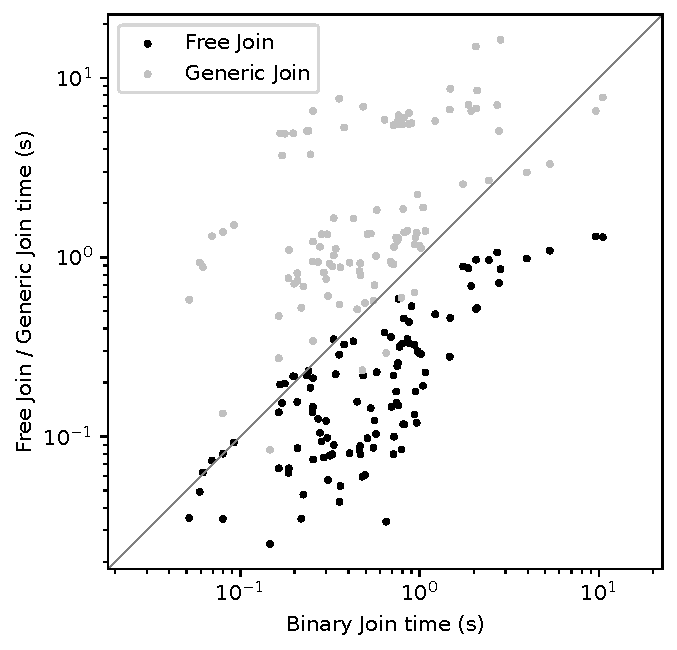
\includegraphics[width=\linewidth]{imdb.pdf}
    \captionof{figure}{Run time comparison on JOB. 
    Each black dot compares the run time of a query on \FJ and binary join, 
    and a black dot below the diagonal means \FJ is faster.
    The gray dots compare \GJ and binary join similarly.
    }
    \label{fig:eval:imdb}
  \end{minipage}%
  \hspace{1em}
  \begin{minipage}[t]{.45\textwidth}
    \centering
    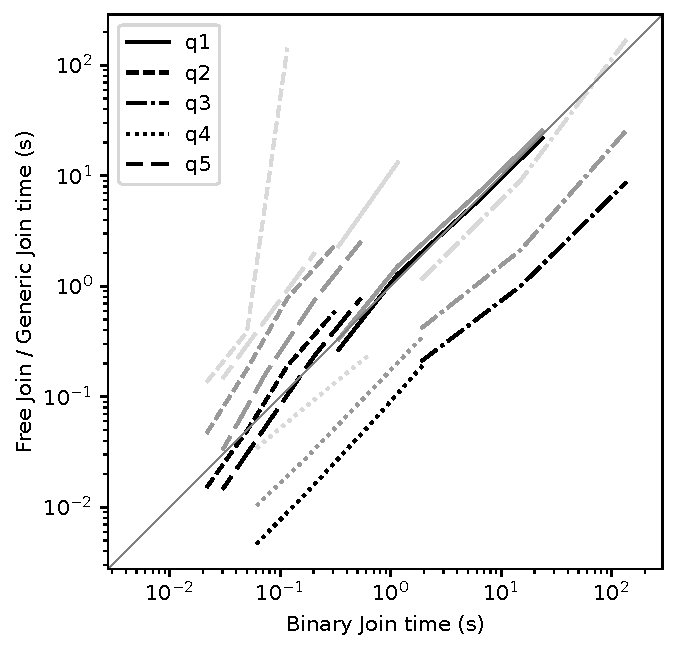
\includegraphics[width=\linewidth]{lsqb-slow.pdf}
    % \captionof{figure}{\FJ and \GJ v.s.\ binary join on LSQB queries.
    % Each line is a query running on increasing scaling factors (0.1-3).
    % Grey lines are for \GJ, and black lines are for \FJ.
    % }
    \captionof{figure}{Run time comparison on LSQB.
    Each line is a query running on increasing scaling factors (0.1, 0.3, 1, 3).
    The black lines compare \FJ with binary join, 
     the gray lines compare our \GJ baseline with binary join, 
     and the light gray lines compare K\`uzu with binary join.
    }
    % Grey lines are for \GJ, and black lines are for \FJ.
    % }
    \label{fig:eval:lsqb}
  \end{minipage}
  \end{figure*}


\subsection{Run time comparison}\label{sec:run-time-comparison}
Our first set of experiments compare the performance of \FJ, \GJ, and binary join
  on the JOB and LSQB benchmarks.
For each query in the benchmarks, we invoke DuckDB to obtain an optimized binary plan,
  and provide the plan to our \FJ and \GJ implementation.
We run LSQB with the scaling factors 0.1, 0.3, 1, and 3, 
  as some queries run out of memory with larger scaling factors.

Figure~\ref{fig:eval:imdb} compares the run time of \FJ and \GJ against binary join on JOB queries.
We see that almost all data points for \FJ are below the diagonal, 
  indicating that \FJ is faster than binary join.
On the other hand, the data points for \GJ are largely above the diagonal, 
  indicating that \GJ is slower than both binary join and \FJ.
On average (geometric mean), \FJ is \imdbavgfjbj faster than binary join 
  and \imdbavgfjgj faster than \GJ.
The maximum speedups of \FJ against binary join and \GJ 
  are \imdbmaxfjbj and \imdbmaxfjgj, respectively, 
  while the minimum speedups are \imdbminfjbj (\imdbmaxbjfj slowdown) and \imdbminfjgj.

We zoom in onto a few interesting queries for a deeper look.
The slowest query under DuckDB is Q13a, taking over 10 seconds to finish.
  \GJ runs slightly faster, taking 7 seconds, 
  whereas \FJ takes just over 1 second.
The query plan for this query reveals the bottleneck for binary join:
  the first 3 binary joins are over 4 very large tables, 
  and two of the joins are many-to-many joins, exploding the 
  intermediate result to contain over 100 million tuples.
However, all 3 joins are on the same attribute;
in other words they are quite  similar to our clover query $Q_\clubsuit$.
As a result, \GJ and \FJ simply intersects the relations 
  on that join attribute, 
  expanding the remaining attributes only after 
  other more selective joins.
This data point appears to confirm a folklore that claims
  \WCOJ algorithms are more resistant to poor query plans.
After all, binary join could have been faster, had the query plan 
  ordered the more selective joins first.
We expand on this point with more experiments evaluating 
  each algorithm's robustness against poor plans in Section~\ref{sec:robustness}.

On a few queries \FJ runs slightly slower than binary join, 
  as shown by the data points over the diagonal.
The binary plans for these queries are all bushy, 
  and each query materializes a large intermediate relation.
We have not spent much effort optimizing for materialization, 
  and we implement a simple strategy: for each intermediate 
  that we need to materialize, we store the tuples containing 
  all base-table attributes in a simple vector.
Future work may explore more efficient materialization strategies, 
  for example only materializing attributes that 
  are needed by future joins.


Figure~\ref{fig:eval:lsqb} compares the performance of \FJ and \GJ against binary join on LSQB queries.
Each line corresponds to one query running on scaling factors 0.1, 0.3, 1, and 3.
The black lines are for \FJ, gray lines for our own \GJ baseline, and light gray lines for K\`uzu.
K\`uzu errors when loading data for SF3;
it did not finish after 10 minutes for q1 SF 1. 
DuckDB also took over 10 minutes running q3 SF 3. 
These instances do not show up in the figure.
We can see K\`uzu takes consistently longer than our \GJ implementation
 on all queries across scaling factors.
This shows that our \GJ implementation is a reasonable baseline to compare against.
On cyclic queries, \FJ is up to 15.45x (q3) faster than binary join, 
  and up to 4.08x (q2) faster than \GJ.
On acyclic queries \FJ is up to 13.07x (q4) and 3.25x (q5) faster than binary join and \GJ, respectively.
On q3 and q4 both \FJ and \GJ consistently outperform binary join on all scaling factors.
q3 contains many cycles, whereas q4 is a star query, so the superior performance of \FJ and \GJ is expected.
% q1, however, is a chain query, where \WCOJ algorithms are expected to be inefficient.
% A deeper look reveals q1 to have an output much larger than its inputs, 
%   but uses a \lstinline|COUNT(*)| at the top.
% An unintended benefit of \GJ and \FJ is that any attributes that 
%   do not participate in a join are not expanded, 
%   so the output result is naturally stored in a \emph{factorized} form.
% We compute the \lstinline|COUNT| aggregate directly on the factorized output, 
%   which is much faster than expanding and counting.
Surprisingly, despite q2 being a cyclic query, 
  \FJ is only slightly faster on smaller inputs
  and is even slightly slower on larger inputs.
This is the opposite of the common believe that \WCOJ algorithms
  should be faster on cyclic queries.
The query plan reveals that there are no skewed joins,
  and so binary join suffers no penalty.
Our experience shows that, in practice, 
  the superiority of \WCOJ algorithms like \FJ and \GJ
  is not solely determined by the cyclicity of the query;
  the presence of skew in the data is another important factor.

\begin{figure}
  \centering
  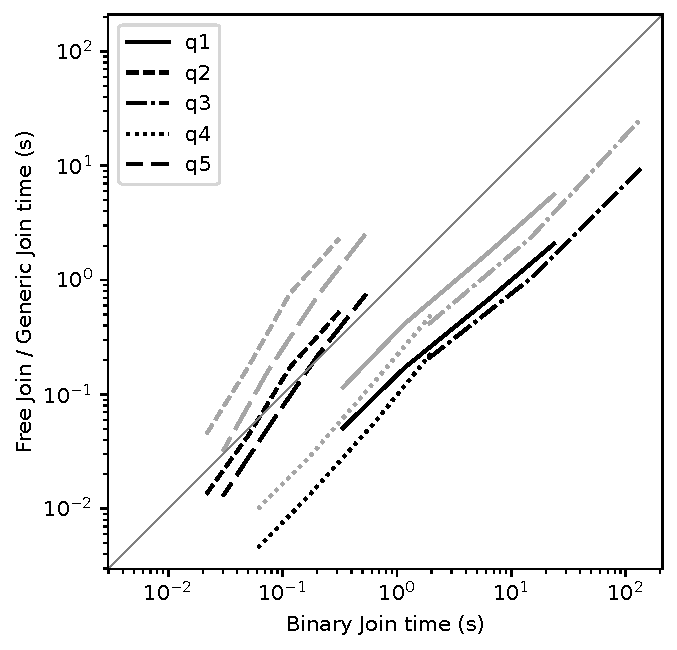
\includegraphics[width=.45\linewidth]{lsqb.pdf}
  \caption{Run time comparison on LSQB w/ factorization.}
  \label{fig:eval:lsqb-factor}
\end{figure}

Unlike the JOB queries, in LSQB the output size (before aggregation)
  is much larger than the input size.
This leads to a large amount of time spent in constructing the output, 
  which involves random accesses to retrieve the data values for each tuple.
We therefore implemented the optimization in Section~\ref{sec:fj-gj-multijoin}
  to factorize the output.
This made q1 significant faster, as shown in Figure~\ref{fig:eval:lsqb-factor},
  while other queries are not affected.

\begin{figure*}
  \centering
  \begin{minipage}{.45\textwidth}
    \centering
    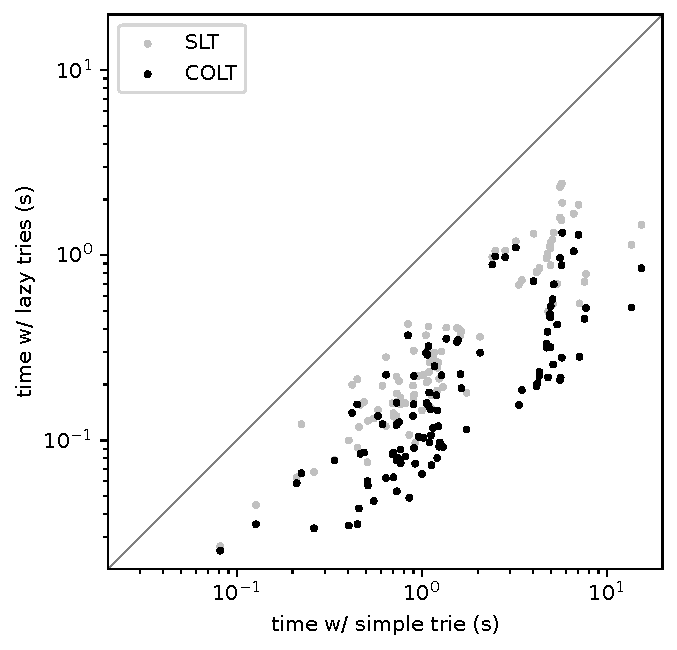
\includegraphics[width=\linewidth]{colt-ab.pdf}
    \captionof{figure}{Impact of \COLT.}
    \label{fig:eval:colt-ab}
  \end{minipage}%
  \hspace{1em}
  \begin{minipage}{.45\textwidth}
    \centering
    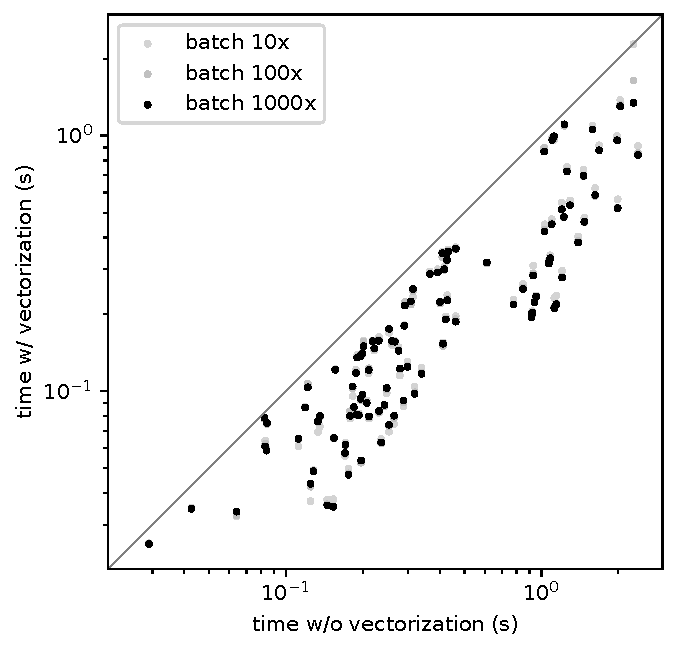
\includegraphics[width=\linewidth]{vec-ab.pdf}
    \captionof{figure}{Impact of vectorization.}
    \label{fig:eval:vec-ab}
  \end{minipage}
  \end{figure*}
  \subsection{Impact of \COLT and Vectorization}
  % \ds{Try to choose section titles that are related to the question
  %   that the section addresses}
The three key ingredients that make \FJ efficient 
  are \begin{enumerate*}
    \item our algorithm to optimize the \FJ plan by factoring,
    \item the \COLT data structure, and
    \item the vectorized execution algorithm.
  \end{enumerate*}
We conduct an ablation study to evaluate the performance impact of these components. 
But if we do not optimize the \FJ plan converted from a binary plan 
  and execute it as-is, \FJ would behave identically to binary join.
Since we have already compared \FJ with binary join in Section~\ref{sec:run-time-comparison},
  we do not repeat it here.
Therefore, our ablation study includes two sets of experiments, 
  evaluating the impact of \COLT and vectorization respectively.



Figure~\ref{fig:eval:colt-ab} compares the run time of \FJ using different trie data structures.
The baseline fully expands each trie ahead of time, and we call this \emph{simple trie}.
Another data structure, \emph{simple lazy trie} (SLT), expands the first level of each trie 
  ahead of time, while expanding the inner levels lazily.
This is the same strategy as proposed by~\cite{DBLP:journals/pvldb/FreitagBSKN20}.
Finally, \COLT is our column-oriented lazy trie.
In all three cases, we use the default vectorization batch size 1000.
The experiments show the average (geometric mean) speedup of \COLT 
  is 1.91x and 8.47x, over SLT and simple trie respectively,
  and the maximum speedup over them is 11.01x and 26.29x, respectively.


Figure~\ref{fig:eval:vec-ab} compares the run time of \FJ using different vectorization batch sizes.
The baseline uses no vectorization, i.e., we set the batch size to 1.
Then we adjust the batch size among 10, 100, and 1000.
The data does not show significant performance differences among
  the different batch sizes -- 
  it appears \emph{any amount of vectorization is better than none}.
For short-running queries, a smaller batch size perform slightly better,
  and for longer running queries a larger batch size wins.
We conjecture this is due to a smaller batch having less overhead, 
  leading to lower latency, 
  while a larger batch size speeds up large joins better,
  leading to better throughput. 
Overall, using the default batch size 1000
  leads to an average (geometric mean) speedup of 2.12x, 
  and a maximum speedup of 5.33x over non-vectorized \FJ.

\begin{figure*}
\begin{minipage}{.48\linewidth}
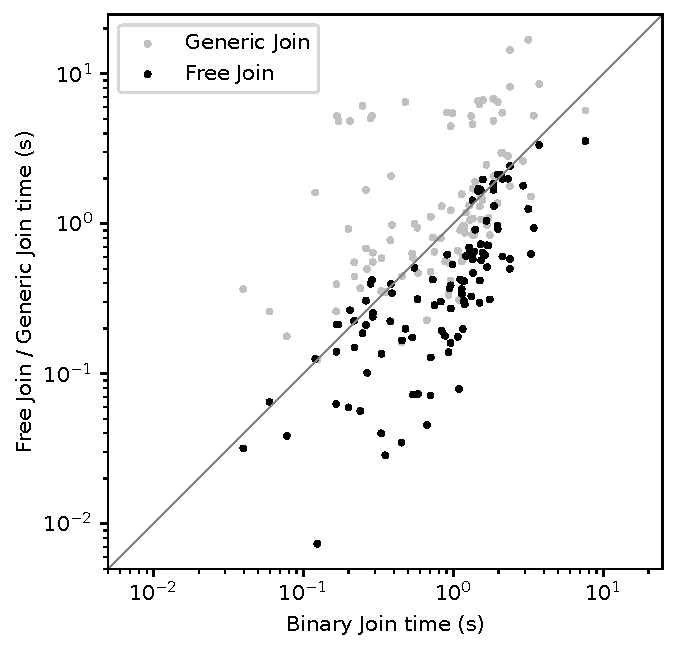
\includegraphics[width=\linewidth]{robust.pdf}
\end{minipage}
\begin{minipage}{.48\textwidth}
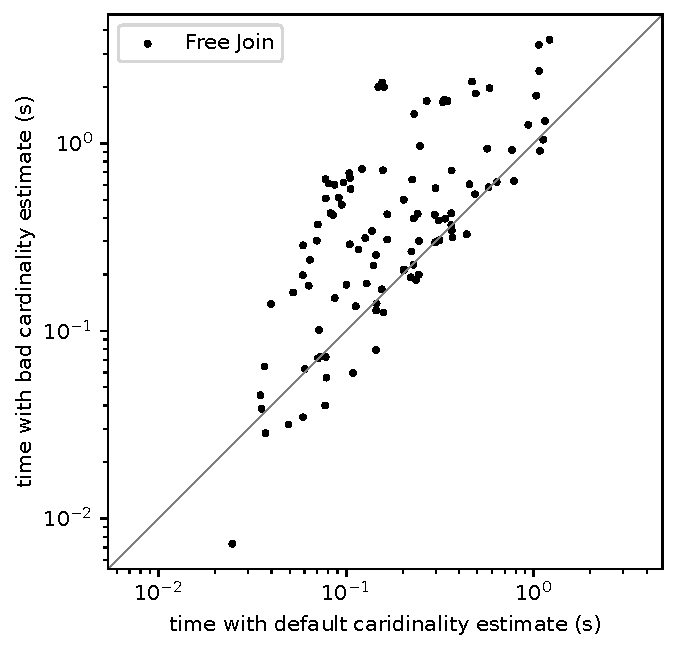
\includegraphics[width=\linewidth]{robust_fj.pdf}
\end{minipage}

\begin{minipage}{.48\textwidth}
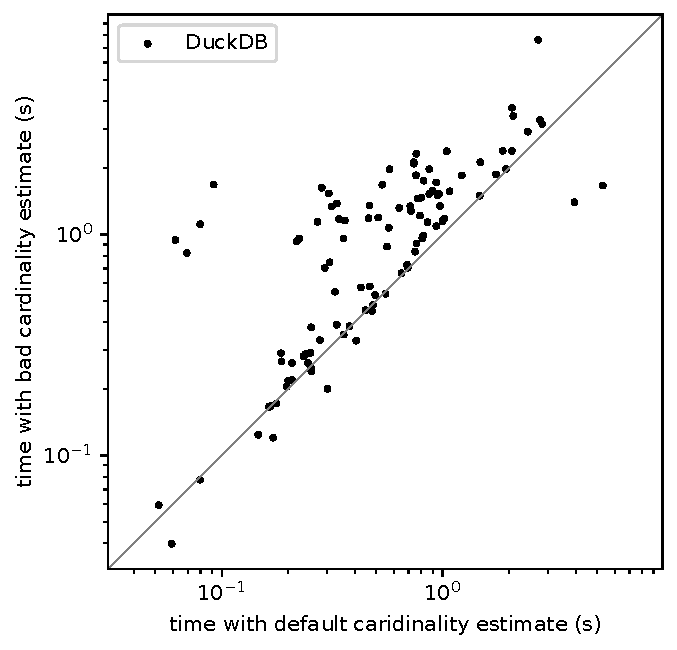
\includegraphics[width=\linewidth]{robust_bj.pdf}
\end{minipage}
\begin{minipage}{.48\textwidth}
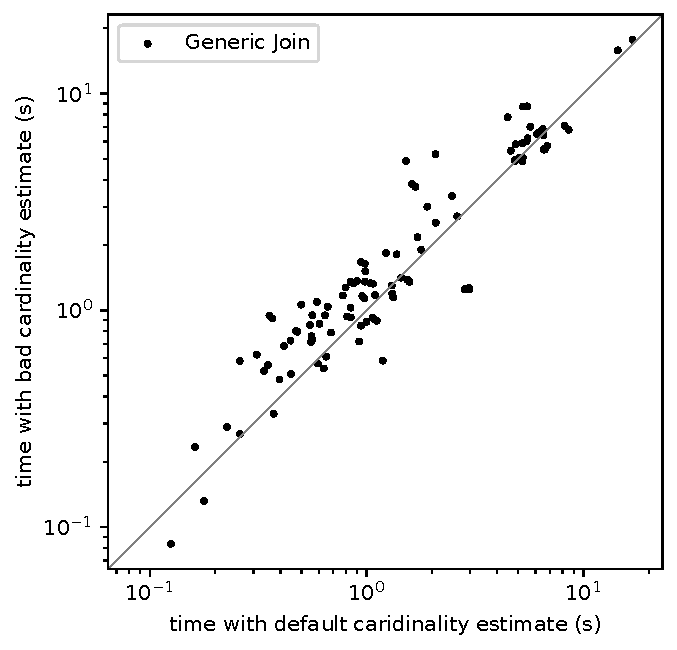
\includegraphics[width=\linewidth]{robust_gj.pdf}
\end{minipage}
\caption{Run time of join algorithms with good and bad cardinality estimates.
The first plot compares the run time of \FJ, \GJ and binary join
  on JOB with bad cardinality estimates.
The remaining three plots compare the run time of each algorithm 
with good and bad cardinality estimates on JOB.
}
\label{fig:sensitivity}
\end{figure*}

\subsection{Robustness Against Poor Plans}\label{sec:robustness}

Our last set of experiments compares \FJ, \GJ and binary join 
  on their sensitivity to the quality of the query plan.
Many believe \WCOJ algorithms suffer less from poor query planning,
  due to its asymptotic guarantees.
Our experience with Q13 from Section~\ref{sec:run-time-comparison}
  also seems to confirm this intuition.
However, our experimental results tell a different story.
As the first plot in Figure~\ref{fig:sensitivity} shows, 
  the relative performance of the three algorithms stays 
  the same with good and bad plans, with \FJ being the fastest,
  \GJ the slowest, and binary join in the middle.
However, as shown in Figure~\ref{fig:sensitivity},
  \FJ seems to slow down as much as binary join 
  when the plan is bad (there are many points far above the diagonal).
It turns out with a poor cardinality estimate, 
  DuckDB routinely outputs bushy plans that materialize large results.
We have noted in Section~\ref{sec:run-time-comparison} that 
  our materialization strategy is simplistic, 
  so with larger intermediates it leads to more severe slowdown.
In comparison, \GJ slows down less (the data points are close to the diagonal).
However, it was the slowest to begin with,
  and since overheads like trie building dominates \GJ's run time, 
  a bad plan does not make it much slower.
Overall, we believe \FJ can be more robust to bad plans with 
  faster materialization.


\clearpage
\addcontentsline{toc}{chapter}{Bibliography}
\singlespacing
\bibliographystyle{alpha}
\bibliography{references}

\end{document}
